% Compile with XeLaTeX; cross-references require multiple passes.
\documentclass[11pt,a4paper]{article}
\usepackage{fontspec}
\IfFontExistsTF{texgyrepagella-regular.otf}
 {\setmainfont{texgyrepagella}[Extension=.otf,UprightFont=*-regular,BoldFont=*-bold,
   ItalicFont=*-italic,BoldItalicFont=*-bolditalic]}
 {\IfFontExistsTF{Palatino Linotype}{\setmainfont{Palatino Linotype}}{\setmainfont{Latin Modern Roman}}}
\linespread{1.05}
\usepackage[english]{babel}
\usepackage{amsmath,amssymb,amsthm,mathtools}
\usepackage{unicode-math}
\IfFontExistsTF{texgyrepagella-math.otf}{\setmathfont{texgyrepagella-math.otf}}{\setmathfont{Latin Modern Math}}
\usepackage[margin=26mm]{geometry}
\IfFileExists{microtype.sty}{\usepackage{microtype}}{}
\IfFileExists{titlesec.sty}{\usepackage[nobottomtitles*]{titlesec}
  \renewcommand{\bottomtitlespace}{.12\textheight}}{}
\usepackage{booktabs,array}
\usepackage[shortlabels]{enumitem}
\usepackage{tikz}
\usetikzlibrary{arrows.meta,positioning}
\usepackage{xcolor}
\usepackage[colorlinks=true,linkcolor={blue!45!black},citecolor={green!35!black},urlcolor={blue!55!black}]{hyperref}

\AtBeginDocument{\renewcommand{\tablename}{Table}}
\setlength{\parindent}{1.15em}
\setlength{\parskip}{0pt plus .35pt}
\setlength{\textfloatsep}{14pt plus 3pt minus 3pt}
\setlength{\intextsep}{12pt plus 3pt minus 3pt}
\setlength{\abovecaptionskip}{6pt}
\setlength{\belowcaptionskip}{2pt}
\AtBeginDocument{\setlength{\abovedisplayskip}{9pt plus 2pt minus 3pt}%
  \setlength{\belowdisplayskip}{9pt plus 2pt minus 3pt}}
\clubpenalty=7000
\widowpenalty=7000
\displaywidowpenalty=3000
\definecolor{btinta}{HTML}{223B49}
\definecolor{bgris}{HTML}{DDE6E7}
\definecolor{bpapel}{HTML}{FFFFFF}
\newcommand{\bcuadricula}[1]{%
  \fill[bpapel] (0,0) rectangle (#1,#1);
  \foreach \r in {1,...,#1}{%
    \foreach \c in {1,...,#1}{%
      \ifodd\numexpr\r+\c\relax
        \fill[bgris] (\c-1,#1-\r) rectangle (\c,#1-\r+1);
      \fi
    }
    \node[font=\scriptsize,anchor=east] at (-.10,#1-\r+.5) {\r};
    \node[font=\scriptsize,anchor=south] at (\r-.5,#1+.06) {\r};
  }
  \foreach \t in {0,...,#1}{\draw[black!45,line width=.3pt] (\t,0)--(\t,#1) (0,\t)--(#1,\t);}
  \draw[btinta,line width=.6pt] (0,0) rectangle (#1,#1);
}
\newcommand{\breina}[3]{%
  \begin{scope}[shift={(#3-.5,#1-#2+.50)}]
    \fill[bpapel] (0,0) circle[radius=.36];
    \fill[btinta] (-.29,.15)--(-.13,.04)--(0,.30)--(.13,.04)--(.29,.15)--(.18,-.15)--(-.18,-.15)--cycle;
    \fill[btinta] (-.21,-.22) rectangle (.21,-.18);
  \end{scope}
}
\newcommand{\bmarca}[3]{\fill[btinta!62] (#3-.5,#1-#2+.50) circle[radius=.055];}

\setlength{\emergencystretch}{2em}
\allowdisplaybreaks[2]
\numberwithin{equation}{section}

\theoremstyle{plain}
\newtheorem{teorema}{Theorem}[section]
\newtheorem{proposicion}[teorema]{Proposition}
\newtheorem{lema}[teorema]{Lemma}
\newtheorem{corolario}[teorema]{Corollary}
\theoremstyle{definition}
\newtheorem{definicion}[teorema]{Definition}
\newtheorem{conjetura}[teorema]{Conjecture}
\theoremstyle{remark}
\newtheorem{observacion}[teorema]{Remark}

% Notation
\newcommand{\eps}{\varepsilon}
\newcommand{\ind}{\mathbf{1}}
\DeclareMathOperator{\pdet}{pdet}
\DeclareMathOperator{\diag}{diag}
\DeclareMathOperator{\tr}{tr}
\newcommand{\Cpred}{C_{\rm pred}}
\newcommand{\Qpred}{Q_{\rm pred}}


\title{The Canonical Predictor for the $n$-Queens Problem:\\ Constant Term and Consistency}
\author{Dilan Steven Mejia\thanks{\href{mailto:mejiadilan@hotmail.com}{\nolinkurl{mejiadilan@hotmail.com}}}}
\date{}

% DOI of the numerical package. An empty value omits the citation.
\newcommand*{\DOIcodigo}{}

\hypersetup{pdftitle={The Canonical Predictor for the n-Queens Problem: Constant Term and Consistency},
 pdfauthor={Dilan Steven Mejia},
 pdfsubject={The n-queens problem. MSC 2020: 05A16, 05A05, 47B10, 82B20},
 pdfkeywords={n-queens problem, asymptotic enumeration, Bethe approximation, regularized determinant, constant term, consistency},
 pdflang={en}}

\begin{document}
\maketitle
\begin{abstract}
\noindent When counting placements of $n$ nonattacking queens, the row and column constraints leave
$n!$ candidate permutations, and the diagonals reduce this number to $Q(n)$.
We construct a deterministic predictor $Q_{\rm pred}(n)$ from a Bethe entropy on square weights.
We prove that its constant term is given by
\[
\begin{aligned}
 \log Q_{\rm pred}(n)-\log n!-n\Phi &\longrightarrow C_{\rm pred},\\
 C_{\rm pred} &=\tfrac12\log2-\tfrac12-\tfrac32I_2-\tfrac12\log{\det}_2(I+J).
\end{aligned}
\]
Here $\Phi=s_1+1$, where $s_1$ is the optimal value at mass one, attained by the profile of mass one;
$I_2$ is the integral of the square of that profile, and $J$ is the Hilbert--Schmidt operator constructed
from it.

\smallskip\noindent When a queen is placed in an empty row, the possible choices split the count
into a sum of residual counts. We prove that the predictor satisfies this recursion up to a factor
$e^{O(k^{-2})}$ in two explicit classes of boards with $k$ empty rows, defined by bounds on the weights,
the diagonal vacancies, and a spectral gap: when $k\ge\delta_0 n$ and, with constants independent of $n/k$,
under a small diagonal mass hypothesis.
Identifying $C_{\rm pred}$ as the constant of the exact count would also require $\log Q(n)-\log Q_{\rm
pred}(n)\to0$; this question remains open.

\smallskip\noindent Numerically, $C_{\rm pred}\approx0.9401$: extrapolating the predictor on finite boards
gives $0.9401$ and a direct evaluation of the formula gives $0.94014$, both with no certified error bound.
In an appendix we prove that, in the rook model, a formula with the same ingredients approximates the
logarithm of the count with error $O(1/k)$, uniformly from positive densities up to the full board.

\medskip\noindent
\textbf{Keywords:} $n$-queens problem; asymptotic enumeration; Bethe approximation;
regularized determinant; constant term; consistency.

\noindent
\textbf{MSC 2020:} 05A16; 05A05; 47B10; 82B20.
\end{abstract}


\section{Introduction}\label{sec:intro}

The $n$-queens problem asks how many ways there are to place $n$ queens on an $n\times n$ board
so that no two attack each other. We denote this number by $Q(n)$. The survey of Bell and
Stevens~\cite{BellStevens} covers the history of the problem and its variants. In a solution, each row
contains one queen. Recording its column as we read the rows from top to bottom gives a
permutation, since no column occurs twice. Figure~\ref{fig:permutaciones} shows why only some of the $n!$
possible
permutations are solutions.

\begin{figure}[htbp]
\centering
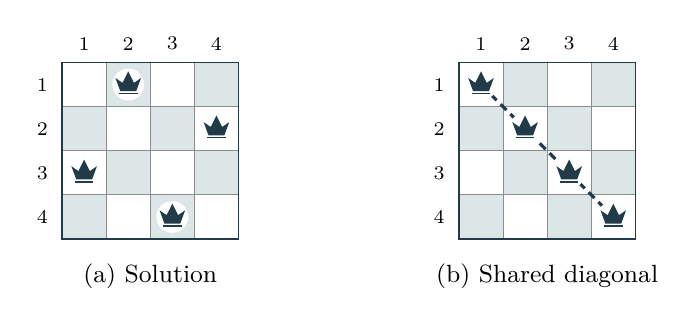
\begin{tikzpicture}[x=5.6mm,y=5.6mm]
  \begin{scope}
    \bcuadricula{4}
    \foreach \r/\c in {1/2,2/4,3/1,4/3} {\breina{4}{\r}{\c}}
    \node[font=\small,anchor=north] at (2,-.35) {(a) Solution};
  \end{scope}
  \begin{scope}[shift={(9,0)}]
    \bcuadricula{4}
    \draw[btinta,densely dashed,line width=1.1pt] (.5,3.5)--(3.5,.5);
    \foreach \r/\c in {1/1,2/2,3/3,4/4} {\breina{4}{\r}{\c}}
    \node[font=\small,anchor=north] at (2,-.35) {(b) Shared diagonal};
  \end{scope}
\end{tikzpicture}
\caption{Two permutations on the same board. Rows are numbered from top to bottom and columns
from left to right, starting at one. In (a) the column sequence is $(2,4,1,3)$: the four
queens also lie on distinct diagonals in each direction. In (b) it is $(1,2,3,4)$:
each row and each column still has one queen, but the diagonal shown contains all four.}
\label{fig:permutaciones}
\end{figure}


By how much do the diagonals reduce these $n!$ possibilities as the board grows?
Simkin~\cite[Theorem~1.1]{Simkin} determined the leading order by a variational principle:
there is a constant $\alpha$ such that
\[
 Q(n)=\bigl((1+o(1))\,n\,e^{-\alpha}\bigr)^n .
\]
Nobel, Agrawal and Boyd~\cite{NAB} bounded $\alpha$ in $[1.944000752,\,1.944001082]$.
Taking logarithms and applying Stirling's formula, Simkin's result gives
\[
 \log Q(n)-\log n!=n(1-\alpha)+o(n).
\]
The remainder $o(n)$ is undetermined. The question motivating this paper concerns the next term:
after subtracting the linear term, does the difference converge, and if so, to what constant?

We construct a deterministic quantity $Q_{\rm pred}(n)$, which we call the predictor and whose constant
term we can calculate. The construction assigns a weight to each square so that each row and
each column sums to one and no diagonal receives more than one. Among the admissible weights
of the model, we choose those that maximize the Bethe entropy (Section~\ref{sec:predictor}). This entropy
contributes the first term of the predictor. The other three terms in Definition~\ref{def:Qpred} are a
local term depending on the square weights, a pseudodeterminant that also depends on how the
lines intersect, and a normalization. The definition requires the maximizer to be interior,
which holds for all sufficiently large $n$ (Section~\ref{sec:P02}).

Passing from the board to the unit square brings in the profile of mass one $\nu_1$ from~\cite{Perfil}.
We write $s_1$ for the optimal value at mass one, attained by that profile, and set $\Phi=s_1+1$.
Section~\ref{sec:preliminares} deduces that $\Phi=1-\alpha$, where $\alpha$ is Simkin's constant;
no proof of the theorems uses this equality. The integral $I_2=\int\nu_1^2$ is taken over the unit square.
Since $\nu_1$ has total mass one,
$I_2\ge1$, with equality only for the constant density: $I_2$ measures how far the profile is from that
density.

\begin{teorema}[Constant term of the predictor]\label{thm:intro-constante}
As $n\to\infty$,
\[
\begin{aligned}
 \log Q_{\rm pred}(n)-\log n!-n\Phi &\longrightarrow C_{\rm pred},\\
 C_{\rm pred} &=\tfrac12\log2-\tfrac12-\tfrac32I_2-\tfrac12\log{\det}_2(I+J),
\end{aligned}
\]
where $J$ is the Hilbert--Schmidt operator constructed from $\nu_1$ in Section~\ref{sec:D03} and
$I+J$ is positive definite.
\end{teorema}

The proof follows the definition term by term. First we approximate the discrete maximizer by the
continuous profile with error $O(1/n)$ (Section~\ref{sec:perfil}). We then identify the contributions of the
entropy and the pseudodeterminant separately and add them to the local term
(Section~\ref{sec:constante}). The theorem is proved in Section~\ref{sec:D05} (Theorem~\ref{thm:constante}).
Of the continuous profile, the proof uses only the properties taken from~\cite{Perfil} that
Section~\ref{sec:preliminares} collects: existence and uniqueness of $\nu_1$, the
factorization~\eqref{eq:factorizacion}, its bounds and a Lipschitz constant. Here $\det_2$ is the
regularized determinant of Hilbert--Schmidt operators, defined in Section~\ref{sec:D04}
(see~\cite[Ch.~9]{Simon}).

The second result answers a question that can already be posed on a small board.
A partial placement leaves a residual board $B$. We choose an empty row $r$ and write
$B+c$ for the residual board left after occupying a legal square $c$ in that row.
If $Q(B)$ counts the completions of $B$, then
\[
 Q(B)=\sum_{c\in r} Q(B+c).
\]
Indeed, each completion uses exactly one of these squares. A legal choice that has no completion
contributes zero to the sum. Figure~\ref{fig:residual} shows this partition on a $5\times5$ board with a
queen in
row~1 and column~2: two legal squares remain in the second row, in columns 4 and~5, and each gives one
summand.

\begin{figure}[htbp]
\centering
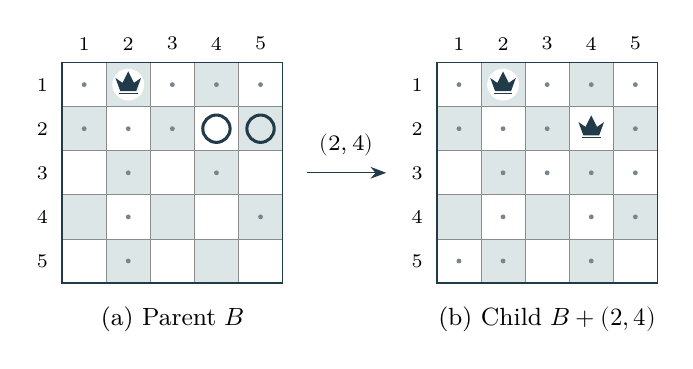
\begin{tikzpicture}[x=5.6mm,y=5.6mm]
 \begin{scope}
  \bcuadricula{5}
  \foreach \r in {1,...,5} {\foreach \c in {1,...,5} {
    \pgfmathtruncatemacro{\ataque}{(\r==1)||(\c==2)||(abs(\r-1)==abs(\c-2))}
    \ifnum\ataque=1\relax\bmarca{5}{\r}{\c}\fi
  }}
  \breina{5}{1}{2}
  \foreach \c in {4,5}{\draw[btinta,line width=1.1pt] (\c-.5,3.5) circle[radius=.31];}
  \node[anchor=north,font=\small] at (2.5,-.32) {(a) Parent $B$};
 \end{scope}
 \draw[-{Stealth[length=2mm]},btinta] (5.55,2.5)--(7.35,2.5);
 \node[font=\footnotesize,above] at (6.45,2.65) {$(2,4)$};
 \begin{scope}[shift={(8.5,0)}]
  \bcuadricula{5}
  \foreach \r in {1,...,5}{\foreach \c in {1,...,5}{
    \pgfmathtruncatemacro{\ataque}{(\r==1)||(\c==2)||(abs(\r-1)==abs(\c-2))||(\r==2)||(\c==4)||%
(abs(\r-2)==abs(\c-4))}
    \ifnum\ataque=1\relax\bmarca{5}{\r}{\c}\fi
  }}
  \breina{5}{1}{2}\breina{5}{2}{4}
  \node[anchor=north,font=\small] at (2.5,-.32) {(b) Child $B+(2,4)$};
 \end{scope}
\end{tikzpicture}
\caption{The exact partition of the count on a small board. The second row of the board on the
left has two legal choices, marked with rings. The arrow follows one of them; the other,
$(2,5)$, gives the second summand of the count. Dots mark occupied squares or squares under attack,
and crowns denote queens already placed. The available squares retain their coordinates.}
\label{fig:residual}
\end{figure}


The predictor assigns to $B$ the value $e^{L(B)}$ (Section~\ref{sec:B3T01}).
We divide the sum of the predictions for the children by the prediction for the parent:
\[
 \rho(B)=\frac{\sum_{c\in r}e^{L(B+c)}}{e^{L(B)}}
        =\sum_{c\in r}e^{L(B+c)-L(B)} .
\]
If the predictor satisfied exactly the same identity as the count, this ratio would be one.
The ratio also depends on the chosen row $r$, which we do not indicate in the notation.
The following theorem bounds the defect on a logarithmic scale and specifies the residual boards for which
the bound holds.

Its statement uses notions made precise in Sections~\ref{sec:insercion} and~\ref{sec:B5T01}.
A residual board with $k$ empty rows also has $k$ empty columns and is missing $k$ queens;
in \cite{Completabilidad} this number is denoted by $h$.
The \emph{Bethe point} of $B$ is the vector of weights $p=(p_e)$, one for each available square
$e$, at which $L(B)$ is evaluated: a stationary point of the Bethe entropy of the residual board
under the row and column constraints. The \emph{mass} of a diagonal in either family is the sum
of the weights of its available squares; its \emph{vacancy} is one minus its mass.
The \emph{row--column Laplacian} is the Laplacian of the graph whose vertices are the empty rows
and columns and in which each available square $e$ is an edge of weight $p_e$ between its row and
its column. Its \emph{gap} is its second smallest eigenvalue, counted with multiplicity.

\begin{teorema}[Second-order consistency]\label{thm:intro-consistencia}
Let $C,\eta,\gamma>0$ and let $B$ be a residual board with $k$ empty rows whose Bethe point $p$ is
stationary and interior, with row and column masses equal to one, $p_e\le C/k$, diagonal vacancies
at least $\eta$, and a gap of at least $\gamma$ for the row--column Laplacian weighted by $p$.
\begin{enumerate}[(a)]
\item For every $\delta_0>0$ there exist $k_0$ and $C_*$, depending only on $\delta_0,C,\eta,\gamma$, such
that if $k\ge\max(k_0,\delta_0n)$, then $|\log\rho(B)|\le C_*/k^2$ for every empty row $r$
(Theorem~\ref{thm:macro} and Corollary~\ref{cor:rho}).
\item There exist $\varepsilon_0$, $k_0$ and $C_*$, independent of $n/k$, such that the same conclusion
holds for $k\ge k_0$ without the condition $k\ge\delta_0n$ if the mass of each diagonal is at most
$\varepsilon_0$ (Theorem~\ref{thm:meso}).
\end{enumerate}
\end{teorema}

Both parts include all legal children of the chosen row. For each child we obtain a unique
stationary point on the small branch, that is, with all its weights less than $1/4$. The first
part requires a fixed fraction of the original rows to remain. The second dispenses with
this condition when the mass of each diagonal is small. In both cases the hypotheses concern
the residual board. The theorem is deterministic: it does not assert that the residual boards
arising when queens are placed at random satisfy these hypotheses.
The class in part~(a) is not empty: for large $n$ it contains the full board
(Corollary~\ref{cor:completo}). For the class in part~(b) we exhibit no residual of queens
with $k=o(n)$ (Section~\ref{sec:B5T05}).

To transfer the first theorem to the exact count, it remains to control a difference:
\[
 R_Q(n)=\log Q(n)-\log Q_{\rm pred}(n).
\]
If $R_Q(n)\to0$, we obtain
\[
 \log Q(n)=\log n!+n\Phi+C_{\rm pred}+o(1).
\]
We do not prove that $R_Q(n)\to0$. Section~\ref{sec:discusion} explains what additional estimates on the
trajectories
and on residual boards with few empty rows this step would require.

Numerically, $C_{\rm pred}\approx0.9401$: over the entire interval for $\alpha$ cited above, fits of the
predictor starting at $n=40$ or $60$ give values between $0.9400$ and $0.9402$, and a direct evaluation of
the formula gives $0.94014$ (Section~\ref{sec:numerico}); none of these figures is certified.
With the reference value $\Phi_0$ from that section, the exact counts for $16\le n\le27$ give values of
$\log Q(n)-\log n!-n\Phi_0$ between $0.913$ and $0.941$.

\subsection*{Relation to previous work}

Luria and Simkin~\cite{LS} obtained a lower bound for the number of queen placements by a greedy
process and absorption. Bowtell and Keevash~\cite{BK} studied the toroidal problem and its
consequences for the ordinary board. Here the construction of the predictor starts from a
different object, the maximum of an entropy on square weights.

The Bethe approximation and its loop corrections have been studied for the permanent of
nonnegative matrices~\cite{Vontobel,WC} and, more generally, for discrete models on graphs~\cite{CC,WF,YFW}.
The Ihara--Bass formula~\cite{Bass}, in the form given by Watanabe and Fukumizu~\cite{WF}, relates the
one-loop correction to a determinant whose size is the number of lines and is the heuristic
origin of the pseudodeterminant in~\eqref{eq:Qpred}.
For toroidal semiqueens, Eberhard, Manners and Mrazović~\cite{EMM19} obtained an asymptotic
formula that includes the constant factor and later treated transversals in quasirandom
Latin squares~\cite{EMM}. Neither model involves both diagonal families of the ordinary board.
Liu, Liao and Wang~\cite{LLW} studied the queens problem as a lattice gas, using Monte Carlo
simulations and tensor networks.
This paper uses the results of~\cite{Perfil} on the profile of mass one. The work in~\cite{Completabilidad}
studies uniformly chosen legal placements missing a fixed number of queens, by a relative
entropy comparison with a reference process and a double count of repairs: the mean
fraction of empty crossings (the intersections of the empty rows and columns) that admit
a queen tends to the reciprocal of the normalization constant of that profile. That result
does not determine the constant term of the exact count.

\subsection*{Organization}

Sections~\ref{sec:preliminares} and~\ref{sec:predictor} proceed from the four lines through a square to the formula for the
predictor. The two questions of the paper are then treated separately. To obtain the constant,
Section~\ref{sec:perfil} compares the finite board with the continuous profile, and Section~\ref{sec:constante}
calculates the terms that survive in the limit. To understand consistency, Section~\ref{sec:insercion}
studies an insertion and Sections~\ref{sec:macro} and~\ref{sec:meso} control its effect in the two regimes of the theorem.

Section~\ref{sec:numerico} compares two evaluations of the constant of the predictor with the values of the
exact count for $16\le n\le27$. Section~\ref{sec:discusion} distinguishes those results from the open question about
$Q(n)$. Appendix~\ref{sec:torres} gives an explicit case in which only the row and column constraints are retained.

\section{Preliminaries}\label{sec:preliminares}

\paragraph{Board and lines.}
The squares of the board are the pairs $(i,j)$ with $1\le i,j\le n$; $i$ is the row and $j$ the column.
There are four families of lines: the rows $R_i$, the columns $C_j$, the diagonals
$D_k=\{i-j=k\}$, $-n<k<n$, and the antidiagonals $A_l=\{i+j-1=l\}$, $0<l<2n$. The families have $n$, $n$,
$2n-1$ and $2n-1$ lines, respectively, for a total of $6n-2$. Each square lies on exactly four lines, one from each
family, and two lines from different families meet in at most one square.
We number rows and columns from one rather than from zero as in~\cite{Perfil}
and~\cite{Completabilidad}: our square $(i,j)$ is their square $(i-1,j-1)$, our diagonal
$D_k$ has difference $k$ in their notation, and our antidiagonal $A_l$ has sum $l-1$.
Figure~\ref{fig:incidencia} shows how to read all four labels for a single square.
\begin{figure}[htbp]
\centering
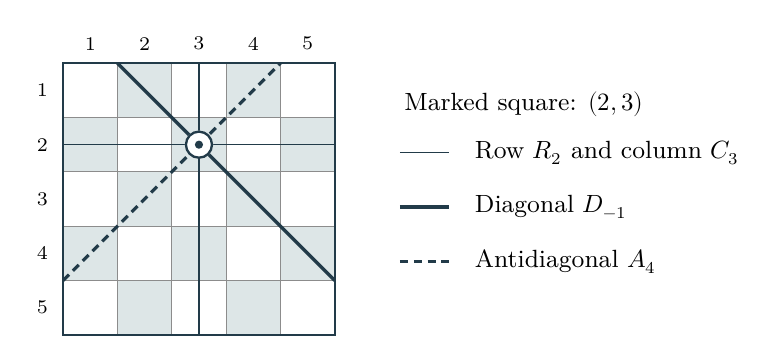
\begin{tikzpicture}[x=6.9mm,y=6.9mm]
 \bcuadricula{5}
 \draw[btinta,thin] (0,3.5)--(5,3.5);
 \draw[btinta,thin] (2.5,0)--(2.5,5);
 \draw[btinta,line width=1.2pt] (1,5)--(5,1);
 \draw[btinta,densely dashed,line width=1.1pt] (0,1)--(4,5);
 \fill[bpapel] (2.5,3.5) circle[radius=.26];
 \draw[btinta,line width=.85pt] (2.5,3.5) circle[radius=.24];
 \fill[btinta] (2.5,3.5) circle[radius=.075];
 \node[anchor=west,font=\small] at (6.1,4.25) {Marked square: $(2,3)$};
 \draw[btinta] (6.2,3.35)--(7.1,3.35);
 \node[anchor=west,font=\small] at (7.4,3.35) {Row $R_2$ and column $C_3$};
 \draw[btinta,line width=1.2pt] (6.2,2.35)--(7.1,2.35);
 \node[anchor=west,font=\small] at (7.4,2.35) {Diagonal $D_{-1}$};
 \draw[btinta,densely dashed,line width=1.1pt] (6.2,1.35)--(7.1,1.35);
 \node[anchor=west,font=\small] at (7.4,1.35) {Antidiagonal $A_4$};
\end{tikzpicture}
\caption{The four lines through $(2,3)$. The diagonal and antidiagonal indices
are determined by the coordinates of the square: $2-3=-1$ and $2+3-1=4$. In the incidence matrix,
the row for this square has a one in the column for each of the four lines shown.}
\label{fig:incidencia}
\end{figure}


We write $A$ for the incidence matrix, with one row per square and one column per line.
For $p\in\mathbb R^{n^2}$ and a line $L$, set
\[
 m_L(p)=\sum_{c\in L}p_c,\qquad h_L(p)=1-m_L(p).
\]

The quantity $m_L$ is the mass assigned to $L$, and the amount $h_L$ by which it falls short of one is its vacancy.
For example, if we assign $1/5$ to every square of the board in the figure, each row sums to one,
whereas diagonal $D_{-1}$ sums to $4/5$: its vacancy is $1/5$.

\paragraph{The continuous profile of mass one.}
To compare boards of different sizes, we divide each coordinate by $n$ and work on a fixed square.
The discrete lines then give projections of the profile.
We follow the notation of~\cite{Perfil}. On the square $[0,1]^2$ with coordinates $(r,c)$, the
projections for the four families are $\ell_R=r$, $\ell_C=c$, $\ell_D=r-c$ and $\ell_A=r+c$, with
values in $I_R=I_C=[0,1]$, $I_D=[-1,1]$ and $I_A=[0,2]$. For a density $\nu\ge0$, $m_f$ is its
projection onto family $f$ and $u_f=1-m_f$ its vacancy. The admissible class at mass one,
$\mathcal A_1$, consists of densities of mass one with $m_f\le1$ almost everywhere, and
\[
 s[\nu]=-3-\int_{[0,1]^2}\nu\log\nu-\sum_{f}\int_{I_f}u_f\log u_f
\]
is the functional of~\cite[(1.1)]{Perfil} at mass one. By~\cite[Theorem~1.1]{Perfil}, $s$ attains its
supremum on $\mathcal A_1$ at a unique density $\nu=\nu_1$. We define the optimal value at mass
one, written in~\cite{Perfil} as $s^*(1)$ and here, as in~\cite{Completabilidad}, as $s_1$, and two
associated quantities:
\begin{equation}\label{eq:s1}
 s_1=s[\nu_1]=\sup_{\nu\in\mathcal A_1}s[\nu],\qquad \Phi=s_1+1,\qquad I_2=\int_{[0,1]^2}\nu_1^2 .
\end{equation}
At mass one the row and column vacancies vanish, so only the diagonal vacancies contribute.
According to~\cite[Remark~2.3]{Perfil}, $s$ then has, on admissible densities, the same expression as the entropy
in Simkin's variational problem~\cite[Definition~2.9]{Simkin}. In~\cite{Simkin}, $-\alpha$ is the maximum of that entropy over
a class of measures defined by closure (Theorem~2.24 and Lemma~2.22); Remark~2.7 of that paper specifies,
for absolutely continuous measures, the relation between this class and the class defined by the projection
constraints. The correspondence above and that remark would give $\alpha=-s_1$, that is, $\Phi=1-\alpha$ and $\log Q(n)=\log n!+n\Phi+o(n)$. We call this
the identification with Simkin's problem. We do not use it in any proof: the definition
$\Phi=s_1+1$ and the theorems on the predictor are independent of it.

By~\cite[Theorems~1.2 and~1.3 and Proposition~5.2]{Perfil}, the profile of mass one factors as
\begin{equation}\label{eq:factorizacion}
 \nu_1(r,c)=b_0\,r_R(r)\,r_C(c)\,u_D(r-c)\,u_A(r+c),
\end{equation}
with $b_0>0$ and continuous, positive Lipschitz functions $r_R,r_C,u_D,u_A$, $\int_0^1r_R=\int_0^1r_C=1$.
In those results, these factors are the limits of the rescaled profile at the full board and
are written $b_0$, $r_{R,0}$, $r_{C,0}$, $u_{D,0}$ and $u_{A,0}$; as in~\cite{Completabilidad},
we omit the subscript except in the constant $b_0$.
The row and column marginals of $\nu_1$ equal one, and $u_f+m_f=1$ for $f=D,A$, where
$m_f$ is the projection of $\nu_1$ onto family $f$. There are positive constants
$c_\nu\le C_\nu$, $\kappa_\nu\le1$ and $L_\nu$ such that
\[
 c_\nu\le\nu_1\le C_\nu,\qquad \kappa_\nu\le u_D,u_A\le1,
\]
and $L_\nu$ is a Lipschitz constant for $\nu_1$ with respect to the maximum metric. Sections~\ref{sec:perfil}
and~\ref{sec:constante} use only these properties of the continuous profile. In those sections we write $\nu$
for $\nu_1$.

\paragraph{Conventions.}
The constants $C,c,M,\eta,\kappa,\dots$ do not depend on $n$ unless stated otherwise;
$O(\cdot)$ and $o(\cdot)$ refer to $n\to\infty$. In Sections~\ref{sec:insercion}
to~\ref{sec:meso} the parameter is the number $k$ of empty rows: there $O(\cdot)$ refers to
$k\to\infty$, and each section specifies what the constants depend on. The letter $h$, which
denotes that number in~\cite{Completabilidad}, is used here for vacancies. In Sections~\ref{sec:perfil}
and~\ref{sec:constante} the equations have labels specific to each subsection, such as (P1.3) or (D2.5).
In the normalization logarithms $\log(4\pi n)$ and $\log(2\pi)$, in Stirling's formula, in the
Slater point of Section~\ref{sec:P01} and in Appendix~\ref{sec:torres}, $\pi$ denotes
$3.14159\ldots$; elsewhere, $\pi=\pi^{(n)}$ is the canonical maximizer and $\pi_c$ the weight of
square $c$. Some letters that have a fixed meaning in~\cite{Perfil}, such as $\rho$, $x$, $\lambda$,
$\ell$, $u$, $F$, $J$, $L$ or $\mathcal H$, denote other objects in some sections of this paper.
We define them where they occur; for example, $\rho(B)$ is not a mass.

\section{The canonical predictor}\label{sec:predictor}

In the exact count, each placement is a list of occupied squares. The predictor uses a different variable:
a weight $p_{ij}$ at each square. The row, column and diagonal sums express the constraints retained by the
model.
Among all admissible assignments of weights, we choose just one: the maximizer of the functional below.

\paragraph{The canonical functional.}
Let $\mathcal D$ denote the union of the two diagonal families, with $|\mathcal D|=4n-2$. Consider the
polytope and the functional
\begin{equation}\label{eq:Kn}
 K_n=\Bigl\{p\in[0,1/4]^{n^2}:\ \sum_jp_{ij}=\sum_ip_{ij}=1,\ m_d(p)\le1\ (d\in\mathcal D)\Bigr\},
\end{equation}
\begin{equation}\label{eq:Hn}
 H_n(p)=\sum_{ij}\bigl\{-p_{ij}\log p_{ij}+3(1-p_{ij})\log(1-p_{ij})\bigr\}-\sum_{d\in\mathcal D}h_d(p)\log
h_d(p),
\end{equation}
with $0\log0=0$. This functional is the Bethe entropy~\cite{YFW} of the system of rows, columns and
diagonals, expressed in the square variables and restricted to fractional placements of total mass $n$.
The cap $p\le1/4$ makes the square term concave.

\begin{lema}[The canonical maximizer]\label{lem:maximizador}
For $n\ge4$, $K_n$ is a nonempty compact convex set, and $H_n$ is continuous on $K_n$ and strictly concave
along every segment in $K_n$. Consequently, $H_n$ has a unique maximizer on $K_n$, which we
denote by $\pi^{(n)}$ and call the canonical maximizer.
\end{lema}
\begin{proof}
The uniform placement $p\equiv1/n$ lies in $K_n$ if $n\ge4$, because each diagonal has at most $n$
squares. We write $H_n(p)=\sum_cf(p_c)+\sum_{d\in\mathcal D}G(m_d(p))$, with
$f(t)=-t\log t+3(1-t)\log(1-t)$ on $[0,1/4]$ and $G(z)=-(1-z)\log(1-z)$ on $[0,1]$. Both functions are
continuous on
their closed intervals, and $f''(t)=-1/t+3/(1-t)<0$ on $(0,1/4)$.

Let $p^0\ne p^1$ in $K_n$, $p^t=(1-t)p^0+tp^1$ and $I=\{c:p^0_c\ne p^1_c\}\ne\emptyset$. For $c\in I$ and
$t\in(0,1)$, $p^t_c$ lies strictly between $p^0_c$ and $p^1_c$, hence in $(0,1/4)$; thus
$t\mapsto f(p^t_c)$ is of class $C^2$ on $(0,1)$ with second derivative $f''(p^t_c)(p^1_c-p^0_c)^2<0$.
Squares outside $I$ give constants. Each $t\mapsto G(m_d(p^t))$ is concave because $G$ is concave
on $[0,1]$ and $m_d$ is affine. The sum $\varphi(t)=H_n(p^t)$ is continuous on $[0,1]$ and strictly concave
on $(0,1)$, hence concave on $[0,1]$. If the strict inequality failed between two points
$t_0<t_1$ of $[0,1]$, $\varphi$ would touch its chord at an interior point of $[t_0,t_1]$ and would be
affine on
that interval, contrary to strict concavity on $(t_0,t_1)$. Existence of the maximizer follows
from compactness, and uniqueness from strict concavity.
\end{proof}

\begin{definicion}\label{def:Hinf}
We say that $(H_\infty)$ holds if the canonical maximizer is interior:
$0<\pi^{(n)}_c<1/4$ for every square $c$ and $h_d(\pi^{(n)})>0$ for every diagonal $d$.
\end{definicion}

Section~\ref{sec:P02} proves that $(H_\infty)$ holds for every $n\ge n_0$, with
$c/n\le\pi^{(n)}_{ij}\le M/n$ and $h_d\ge\eta$ for positive constants $c$, $M$ and $\eta$
(see~(P2.7)). The threshold $n_0$ given by that proof is very large (end of Section~\ref{sec:P02}).
For $n=4$ the hypothesis fails, and for $n=5$ the numerical computation indicates that it fails as well
(Section~\ref{sec:discusion}); for $6\le n<n_0$ it is not proved, and for the sizes of
Section~\ref{sec:numerico} it is checked numerically.
Below we write $\pi=\pi^{(n)}$ when there is no ambiguity.

\paragraph{The pseudodeterminant and the local term.}
Let $n\ge4$ be such that its maximizer satisfies $(H_\infty)$. Set
\begin{equation}\label{eq:gS}
 g_c=\frac{\pi_c(1-\pi_c)}{1-4\pi_c},\qquad
 S_n=\operatorname{diag}(0_R,0_C,h_D,h_A)+A^T\operatorname{diag}(g)A,
\end{equation}
a symmetric matrix indexed by the $6n-2$ lines, and set $v_0=(\mathbf1_R,-\mathbf1_C,0_D,0_A)$. The
quadratic form of $S_n$ is a sum of squares whose weights, $h_d$ and $g_c$, are positive by
$(H_\infty)$. If it vanishes at a vector
$x=(x_R,x_C,x_D,x_A)$, then $x_D=0$, $x_A=0$ and $x_{R,i}+x_{C,j}=0$ for each square $(i,j)$. Its
kernel is therefore the line spanned by $v_0$, and $S_n$ is positive definite on $v_0^\perp$. For
$n\ge n_0$, Section~\ref{sec:P03} also gives a uniform gap. We call the direction $v_0$, the discrete
analogue of the neutral mode $(1,-1,0,0)$
in~\cite[Section~7.2]{Perfil}, and its analogue on residual boards the \emph{gauge}:
since $Av_0=0$, adding a multiple of $v_0$ to a vector indexed by the lines does not change its
sums at the squares. Fixing the gauge means choosing a representative, for instance in $v_0^\perp$. The
pseudodeterminant
$\operatorname{pdet}S_n$ is the product of its nonzero eigenvalues. The local term is
\[
 L_n=-\frac12\sum_{ij}\bigl[\log(1-4\pi_{ij})-4\log(1-\pi_{ij})\bigr],
\]
as in~(LC1).

\begin{definicion}[Canonical predictor]\label{def:Qpred}
For $n\ge4$ satisfying $(H_\infty)$,
\begin{equation}\label{eq:Qpred}
 \log Q_{\rm pred}(n)=H_n(\pi^{(n)})+L_n-\tfrac12\log\operatorname{pdet}S_n+\tfrac12\log(4\pi n).
\end{equation}
\end{definicion}

\begin{observacion}[Origin of the definition]
Of the four terms in the definition, the first is the Bethe entropy at its maximum. The other
three correspond, heuristically, to two further ingredients: the one-loop correction to the
Bethe approximation, expressed as a determinant of the Hessian matrix by the
Ihara--Bass formula in the form of Watanabe and Fukumizu~\cite{Bass,WF}, and the Gaussian normalization of
the
zero mode that imposes equality between the number of empty rows and the number of empty columns. For these
approximations for permanents and systems on graphs, see~\cite{CC,ChertkovYedidia,Vontobel}, and for
loop corrections to the Bethe approximation,~\cite{MontanariRizzo}. In the rook model,
a formula with the same three ingredients approximates the logarithm of the count with error
$O(1/k)$ up to the full board (Appendix~\ref{sec:torres}). In this paper \eqref{eq:Qpred} is
only a definition: no proof uses this interpretation or the appendix.
\end{observacion}

For the residual boards that arise as queens are placed one at a time, the predictor $L(B)$ is defined in
Section~\ref{sec:B3T01}, with the same functional, the canonical determinant of the residual board and the
normalization $\tfrac12\log(2\pi)$ per component. On the full board, $L(B)$ coincides with
$\log Q_{\rm pred}(n)$ (Lemma~\ref{lem:puente}).

\section{The discrete canonical profile}\label{sec:perfil}

Passing from the board to the unit square requires comparing quantities on the same scale.
Since the weights of the $n$ squares in each row sum to one, their average is $1/n$. We therefore compare
the rescaled weight $n\pi_{ij}$, rather than the original weight, with the value of $\nu_1$ at the center of
the square.

We first need to ensure that the maximizer stays away from the endpoints in the precise sense of
Section~\ref{sec:P02}: its weights lie between $c/n$ and $M/n$, and the diagonal vacancies
have a positive lower bound. Section~\ref{sec:P01} lays the groundwork for these bounds
by constructing a Slater point, that is, a feasible point satisfying the diagonal and square constraints
strictly.
We use these bounds to control the spectrum of $S_n$ in Section~\ref{sec:P03} and to expand
the local term in Section~\ref{sec:P04}. Finally, Sections~\ref{sec:P05}
and~\ref{sec:P06} establish the stated comparison with uniform error $O(1/n)$.

\subsection{A Slater point and a bound on the cap multipliers}\label{sec:P01}
From Lemma~\ref{lem:maximizador} we use only the existence and uniqueness of the canonical maximizer.
We neither assume that it lies in the interior nor assert that its weights coincide with the square
occupancy probabilities in a solution chosen uniformly at random.
Recall that $\mathcal D$ is the union of the two diagonal families of the board,
with $|\mathcal D|=4n-2$, and that
\[
 m_d(p)=\sum_{c\in d}p_c,\qquad h_d(p)=1-m_d(p).
\]
The polytope $K_n$ and the functional $H_n$ are those of~\eqref{eq:Kn} and~\eqref{eq:Hn}, with the
convention
$0\log0=0$. We denote by $p=\pi^{(n)}$ the unique maximizer of $H_n$ on $K_n$.

\paragraph{A Slater point for $n\ge32$.}
Let $r_i=(i-1/2)/n$ and
\[
 q_{ij}=\frac1n\left[1-\frac15\cos(2\pi r_i)\cos(2\pi r_j)\right].
\]
The sum of the cosines at the $n$ midpoints is zero for $n\ge2$.
Thus the row and column sums of $q$ are exactly one, and
$4/(5n)\le q_{ij}\le6/(5n)$.
The strictly admissible density $\nu^\sharp(r,c)=1-\frac15\cos(2\pi r)\cos(2\pi c)$
from~\cite[Remark~2.4]{Perfil} has, for $0\le d\le1$, the marginal
\[
 m_D[\nu^\sharp](d)=1-d-\frac15\left[
       \frac{1-d}{2}\cos(2\pi d)-\frac{\sin(2\pi d)}{4\pi}\right].
\]
Its derivative is at most $-1+(1+\pi)/5<0$, so $m_D[\nu^\sharp]\le9/10$.
By symmetry, the same bound holds throughout both families.
Each diagonal sum of $q$ is a midpoint quadrature for
$\nu^\sharp$ on the corresponding fiber, whose endpoints are multiples of $1/n$.
The parameter length of the fiber is at most one, and the Lipschitz constant along it
is at most $4\pi/5$. The quadrature error is thus
at most $(4\pi/5)/(2n)\le1/20$ for $n\ge32$, using $\pi<4$.
Consequently, with $M_0=6/5$ and $\kappa=1/20$,
\[
 q_{ij}\le M_0/n<1/8,\qquad h_d(q)\ge\kappa.       \tag{P1.1}
\]
This gives a Slater point in the affine space defined by the row and column sums.

\paragraph{Positivity in the presence of the cap.}
Take $p(t)=(1-t)p+tq$. If $p_c=0$, its spatial entropy contributes
$-q_c t\log t+O(t)$ to $H_n(p(t))-H_n(p)$. If $h_d(p)=0$, its
diagonal entropy contributes $-h_d(q)t\log t+O(t)$. The other entropy terms
contribute $O(t)$, as does $3(1-p)\log(1-p)$, whose derivative
is bounded on $[0,1/4]$. If any of these equalities holds, the
difference is $-At\log t+O(t)>0$ for small $t>0$, with $A>0$,
contradicting maximality. Hence
\[
 p_{ij}>0,\qquad h_d(p)>0.                         \tag{P1.2}
\]

\paragraph{Optimality conditions with cap multipliers.}
By (P1.2), the functional is differentiable near $p$, and the only potentially
active inequalities are $p_{ij}\le1/4$.
Slater's condition gives finite multipliers $\alpha_i,\beta_j$ and
$\mu_{ij}\ge0$. One of the row and column equalities is redundant and is omitted
when applying the Karush--Kuhn--Tucker (KKT) conditions~\cite[Ch.~5]{BV}. If $D(i,j),A(i,j)$ are the
two diagonals through the square, we obtain
\[
 -\log p_{ij}-3\log(1-p_{ij})+\log h_{D(i,j)}+\log h_{A(i,j)}-2
 =\alpha_i+\beta_j+\mu_{ij},\quad
 \mu_{ij}(1/4-p_{ij})=0.                          \tag{P1.3}
\]
Let $x_{ij}=np_{ij}$, $\ell_d=-\log h_d(p)\ge0$, and
$d_0=3\log(4/3)$. Multiplying (P1.3) by $q_{ij}-p_{ij}$ and
summing cancels the terms from the equality constraints and the constant $-2$. This gives
\[
 0=E+F+Q+U,                                      \tag{P1.4}
\]
\[
 E=\sum_{ij}(p_{ij}-q_{ij})\log x_{ij},\qquad
 F=3\sum_{ij}(p_{ij}-q_{ij})\log(1-p_{ij}),
\]
\[
 Q=\sum_{d\in\mathcal D}(h_d(q)-h_d(p))\ell_d,\qquad
 U=\sum_{ij}\mu_{ij}(1/4-q_{ij}).
\]
In particular, $U$ enters with a plus sign: by complementarity, the derivative in the direction $q-p$
is $-U$.

\paragraph{A global bound including the cap multipliers.}
Convexity gives $\sum p_{ij}\log(np_{ij})\ge0$. Moreover,
\[
 \sum q_{ij}\log x_{ij}\le\frac{M_0}{n}\sum\log^+x_{ij}
 \le\frac{M_0}{n}\sum x_{ij}=M_0n,
\]
so $E\ge-M_0n$. Since $\log(1-p)\le0$,
\[
 F\ge3\sum p_{ij}\log(1-p_{ij})\ge-d_0n.
\]
The inequality $h(-\log h)\le1/e$ and (P1.1) give
\[
 Q\ge\kappa\sum_d\ell_d-4n/e,\qquad
 U\ge\frac18\sum_{ij}\mu_{ij}.
\]
By (P1.4), setting $C_0=M_0+d_0+4/e$ yields
\[
 \kappa\sum_d\ell_d+\frac18\sum_{ij}\mu_{ij}\le C_0n.
\]
Since $\kappa\le1/8$, setting $T=C_0/\kappa$ gives
\[
 \frac1n\left(\sum_d\ell_d+\sum_{ij}\mu_{ij}\right)\le T.    \tag{P1.5}
\]
This estimate does not assume that any multiplier $\mu$ vanishes.

\subsection{Uniform bounds on weights and vacancies, and interiority}\label{sec:P02}
We retain the notation of Section~\ref{sec:P01}, in particular
$n\ge32$, $\kappa=1/20$, $M_0=6/5$, $d_0=3\log(4/3)$, and
$T=(M_0+d_0+4/e)/\kappa$.

\paragraph{Factorization with the multiplier retained.}
Equation (P1.3) admits the factorization
\[
 x_{ij}=B R_i C_j K_{ij},\qquad
 K_{ij}=h_{D(i,j)}h_{A(i,j)}e^{-\mu_{ij}}(1-p_{ij})^{-3},
                                                               \tag{P2.1}
\]
with positive factors and geometric normalizations
\[
 \frac1n\sum_i\log R_i=\frac1n\sum_j\log C_j=0.
\]
For example, these factors are obtained by dividing $e^{-\alpha_i}$ and
$e^{-\beta_j}$ by their geometric means and absorbing into $B$
these two scalar factors together with $ne^{-2}$.
Each row meets each diagonal in either family at most once.
Thus (P1.5) and the inequality $(1-p)^{-3}\ge1$ give
\[
 \frac1n\sum_j\log K_{ij}\ge-T.
\]
The same property holds for each column:
\[
 \frac1n\sum_i\log K_{ij}\ge-T.                  \tag{P2.2}
\]
Here we use the global sum of $\mu$: the sum of its values in any
row or column is at most the global sum.

\paragraph{Control of the factors without a pointwise vacancy assumption.}
Jensen's inequality, the geometric normalizations, and the row sums give
\[
 1=B R_i\frac1n\sum_j C_jK_{ij}\ge B R_i e^{-T}.
\]
Applying the same argument to the columns gives
\[
 R_i,C_j\le e^T/B.                               \tag{P2.3}
\]
On the other hand, $\log K_{ij}\le d_0$, since $h_d\le1$,
$\mu_{ij}\ge0$, and $p_{ij}\le1/4$.
We multiply the logarithm of (P2.1) by $p_{ij}$ and sum.
The contributions of $\log R_i$ and $\log C_j$ vanish because the
row and column sums are one and the logarithms of the factors in each family sum
to zero. By the convexity used in Section~\ref{sec:P01},
\[
 n\log B=\sum_{ij}p_{ij}\log(np_{ij})
               -\sum_{ij}p_{ij}\log K_{ij}\ge-d_0n.
\]
Thus $B\ge e^{-d_0}$. From (P2.3) we deduce the bound
\[
 B R_i C_j(1-p_{ij})^{-3}
 \le e^{2T+d_0}/B\le e^{2T+2d_0}=:M.             \tag{P2.4}
\]
In (P2.1) all the factors $h_d,e^{-\mu_{ij}}$ are at most
one. Hence, with the caps still in place,
\[
             0<p_{ij}\le M/n.                    \tag{P2.5}
\]

\paragraph{Uniform vacancy bounds.}
Fix a diagonal $d$ in the first family. By (P2.1) and (P2.4),
\[
 m_d(p)=\frac{h_d}{n}\sum_{(i,j)\in d}
 B R_i C_j h_{A(i,j)}e^{-\mu_{ij}}(1-p_{ij})^{-3}
 \le M h_d\frac{|d|}{n}\le M h_d.
\]
The same argument applies to the second family.
Since $m_d=1-h_d$, it follows that for all diagonals
\[
                 h_d\ge\eta:=\frac1{1+M}.        \tag{P2.6}
\]
This conclusion also holds before the cap is removed.

\paragraph{Removal of the cap and a lower bound.}
For
\[
 n\ge n_0:=\max\{32,\lfloor4M\rfloor+1\},
\]
(P2.5) implies $p_{ij}<1/4$. Complementarity then gives
$\mu_{ij}=0$ at every square.
This establishes hypothesis $(H_\infty)$ of Definition~\ref{def:Hinf} and
the uniform bounds. In fact, bounds (P2.5) and
(P2.6) already hold for every $n\ge32$.
For $n\ge n_0$ we also have a lower bound of order $1/n$.
By $K_{ij}\le e^{d_0}$ and (P2.3), the row equation implies
\[
 R_i=\left(B\frac1n\sum_jC_jK_{ij}\right)^{-1}
       \ge e^{-(T+d_0)};
\]
and similarly $C_j\ge e^{-(T+d_0)}$.
Once $\mu=0$, (P2.6) gives $K_{ij}\ge\eta^2$. Together with
$B\ge e^{-d_0}$, this proves
\[
 \frac{c}{n}\le p_{ij}\le\frac Mn,\qquad
 c:=\eta^2e^{-2T-3d_0}>0,
 \qquad h_d\ge\eta.                              \tag{P2.7}
\]

\paragraph{Size of the constants.}
With $\kappa=1/20$, $M_0=6/5$ and $d_0=3\log(4/3)$ we obtain $T\approx70.7$,
$M=e^{2T+2d_0}\approx1.4\cdot10^{62}$, $n_0\approx5.7\cdot10^{62}$ and
$\eta\approx7\cdot10^{-63}$; the constant in~(P2.7) that bounds $n\pi_c$ from below is
$c=\eta^2e^{-2T-3d_0}\approx1.5\cdot10^{-187}$. These constants suffice for the asymptotic statements,
but they do not describe the boards that can be computed: for the ten sizes in Table~\ref{tab:predictor},
from $n=20$ to $n=240$, the numerical solution of Section~\ref{sec:numerico} gives
$0.45\le n\pi_c\le1.41$ and $h_d\ge0.174$. For $6\le n<n_0$ the interiority of the canonical
maximizer is not proved.

\subsection{A uniform gap for the reduced canonical operator}\label{sec:P03}
We use only the deterministic bounds from Section~\ref{sec:P02}.
Let $n$ be large enough that
\[
 c/n\le\pi_{ij}\le M/n\le1/8,\qquad h_D,h_A\ge\eta>0.
\]
The symbols $c,M,\eta$ denote constants, not square indices.
The incidence matrix $A$ has one row per square and one column per line.
Set
\[
 g_{ij}=\frac{\pi_{ij}(1-\pi_{ij})}{1-4\pi_{ij}},\quad
 S=\operatorname{diag}(0_R,0_C,h_D,h_A)+A^T\operatorname{diag}(g)A.
                                                        \tag{G1}
\]
Then $c/n\le g_{ij}\le2M/n$.
We use ordinary Euclidean norms on the $6n-2$ lines.

\begin{proposicion}
The kernel of $S$ is exactly
$\operatorname{span}\{v_0\}$, where
$v_0=(\mathbf1_R,-\mathbf1_C,0_D,0_A)$.
On $v_0^\perp$ we have
\[
 \gamma\|v\|^2\le v^TSv\le(1+8M)\|v\|^2,
 \qquad \gamma=\min\{c/2,\eta/5\}>0.               \tag{G2}
\]
The constants are independent of $n$.
\end{proposicion}
\begin{proof}
Write $v=(r_i,t_j,d_k,a_l)$ and
$s_{ij}=r_i+t_j+d_{i-j}+a_{i+j-1}$.
The condition $v\perp v_0$ is equivalent to $\sum_i r_i=\sum_jt_j$.
Hence
\[
 \frac1n\sum_{ij}(r_i+t_j)^2
 =\sum_i r_i^2+\sum_jt_j^2+
       \frac2n\left(\sum_i r_i\right)^2
 \ge\|r\|^2+\|t\|^2.
\]
The inequality $(s-d-a)^2\le2s^2+4(d^2+a^2)$
and the fact that each diagonal contains at most $n$ squares
give
\[
 \|v\|^2\le\frac2n\sum_{ij}s_{ij}^2
                        +5(\|d\|^2+\|a\|^2).     \tag{G3}
\]
By (G1),
\[
 v^TSv\ge\frac cn\sum s_{ij}^2+
                          \eta(\|d\|^2+\|a\|^2),
\]
which proves the lower bound. Moreover,
$s_{ij}^2\le4(r_i^2+t_j^2+d_{i-j}^2+a_{i+j-1}^2)$.
Each line contains at most $n$ squares, so
$\sum s_{ij}^2\le4n\|v\|^2$. Since $h_D,h_A\le1$,
the upper bound follows.
Finally, $Sv_0=0$. If $v^TSv=0$, the positivity of
$g,h_D,h_A$ forces $d=a=0$ and $r_i+t_j=0$ for all $i,j$.
Thus $r$ is constant and $t$ is its negative. There are no other null vectors.
\end{proof}

\paragraph{Consequence.}
The inverse of $S$ on $v_0^\perp$ has spectral norm
at most $\gamma^{-1}$, with $\gamma$ independent of $n$.

\subsection{The local term in the canonical formula}\label{sec:P04}
Take $n$ sufficiently large, in particular $n\ge8M$.
We distinguish a consequence of Section~\ref{sec:P02} from one that requires
comparison with the continuous profile (Sections~\ref{sec:P05} and~\ref{sec:P06}).
The local term is
\[
 L_n=-\frac12\sum_{ij}
       [\log(1-4\pi_{ij})-4\log(1-\pi_{ij})].       \tag{LC1}
\]
For $0\le t\le1/8$, the convergent scalar series give
\[
 -\tfrac12[\log(1-4t)-4\log(1-t)]
   =\frac12\sum_{m\ge2}\frac{4^m-4}{m}t^m.
\]
The quadratic term is $3t^2$, and the remaining terms are positive.
Their sum is bounded by
\[
 \frac12\sum_{m\ge3}(4t)^m
       =\frac{32t^3}{1-4t}\le64t^3.
\]
Using $\pi\le M/n$ and $\sum\pi=n$ gives
\[
 0\le L_n-3\sum_{ij}\pi_{ij}^2
       \le64\sum\pi_{ij}^3\le\frac{64M^2}{n}.      \tag{LC2}
\]
Estimate (LC2) is a local expansion on the scale $\pi=O(1/n)$.

\paragraph{From the local term to the continuous profile.}
If $\nu_1$ is the bounded Lipschitz continuous profile and
\[
 \max_{ij}|n\pi_{ij}-\nu_1((i-1/2)/n,(j-1/2)/n)|=O(1/n),
                                                        \tag{LC3}
\]
then
\[
 \sum_{ij}\pi_{ij}^2
       =\int_{[0,1]^2}\nu_1(r,c)^2\,dr\,dc+O(1/n).
\]
Indeed, the difference between the squares of the profiles
is uniformly $O(1/n)$, and the two-dimensional quadrature
of a Lipschitz function has error $O(1/n)$.
By (LC2),
\[
 L_n=3\int_{[0,1]^2}\nu_1^2+O(1/n).               \tag{LC4}
\]
This is only one of the summands in $\log Q_{\rm pred}$. The contributions of the entropy and
the pseudodeterminant are studied in Section~\ref{sec:constante}.

Sections~\ref{sec:P05} and~\ref{sec:P06} prove (LC3) for the canonical maximizer,
so (LC4) applies to it.

\subsection{Comparison with the continuous profile: the system and its residual}\label{sec:P05}
\paragraph{Initial data.}
Sections~\ref{sec:P01} and~\ref{sec:P02} give, for the canonical maximizer $\pi$ and
$n\ge n_0$, where the threshold is that of Section~\ref{sec:P02},
\[
 c\le\rho^*_{ij}:=n\pi_{ij}\le M,\qquad h_D^*,h_A^*\ge\eta>0.
                                                        \tag{TR1}
\]
For the continuous profile of mass one, we use only its factorization, its equations,
and its positivity and Lipschitz bounds (Section~\ref{sec:preliminares}):
\[
 \nu_1(r,c)=b_0 r_R(r)r_C(c)u_D(r-c)u_A(r+c),\quad
 c_\nu\le\nu_1\le C_\nu,\quad \kappa_\nu\le u_D,u_A\le1.
                                                        \tag{TR2}
\]
Its row and column marginals equal one, and $u_f+T_f\nu_1=1$ for $f=D,A$, where $T_f\nu_1=m_f$ is
the projection of $\nu_1$ onto family $f$.
Recall that $L_\nu$ is a Lipschitz constant for $\nu_1$ with respect to the maximum metric.

\paragraph{Grid, operators, and gauge.}
Set $x_i=(i-1/2)/n$. The lines $D_k$ and $A_l$ have parameters
$k/n$ and $l/n$, with $k=i-j$ and $l=i+j-1$ at square $(i,j)$.
The four families consist of $n,n,2n-1,2n-1$ lines, respectively. Define
\[
 (\mathcal R_f p)_\ell=\frac1n\sum_{(i,j)\in\ell}p_{ij},\qquad
 (\mathcal T z)_{ij}=z_{R,i}+z_{C,j}+z_{D,i-j}+z_{A,i+j-1}.
                                                        \tag{TR3}
\]
Write $\mathcal R=(\mathcal R_R,\mathcal R_C,
\mathcal R_D,\mathcal R_A)$. The inner products are
$\langle p,q\rangle_\square=n^{-2}\sum pq$ and
$\langle h,k\rangle_\ell=n^{-1}\sum_{f,\ell}h_{f,\ell}k_{f,\ell}$,
so $\mathcal R^*=\mathcal T$. We use the same space for the domain and range:
\[
 E_n=\{z:\ \sum_i z_{R,i}=\sum_j z_{C,j}\}=v_0^\perp,\qquad
 v_0=(\mathbf1_R,-\mathbf1_C,0_D,0_A).
                                                        \tag{TR4}
\]
Every potential can be moved into $E_n$ by subtracting $\tau v_0$, where
$\tau=(\overline z_R-\overline z_C)/2$. This leaves $\mathcal Tz$ unchanged.

\paragraph{The small root and the exact system.}
Let $\psi_n(t)=t(1-t/n)^3$. Since
$\psi_n'(t)=(1-t/n)^2(1-4t/n)>0$ for $0<t<n/4$,
its inverse on this branch, denoted by $\chi_n$, is unique and smooth.
When the arguments lie in the image of this branch, set
\[
 \rho(z)_{ij}=\chi_n(e^{(\mathcal Tz)_{ij}}),\qquad
 u_D(z)=e^{z_D},\quad u_A(z)=e^{z_A},
\]
\[
 F_n(z)=(\mathcal R_R\rho(z)-1,\mathcal R_C\rho(z)-1,
 u_D(z)+\mathcal R_D\rho(z)-1,u_A(z)+\mathcal R_A\rho(z)-1).
                                                        \tag{TR5}
\]
We always have $F_n(z)\in E_n$. The sums of its R and C components
are exactly equal because both sum to $n^{-1}\sum_{ij}\rho(z)_{ij}-n$.

\paragraph{The canonical maximizer as a solution of the system.}
By Section~\ref{sec:P02}, no cap is active and all the multipliers $\mu_{ij}$ in (P1.3) vanish.
Before fixing the gauge, take
\[
 z^*_{R,i}=\tfrac12\log n-\alpha_i-1,\quad
 z^*_{C,j}=\tfrac12\log n-\beta_j-1,\quad
 z_D^*=\log h_D^*,\quad z_A^*=\log h_A^*.
\]
With this choice, (P1.3) gives $\psi_n(\rho^*_{ij})=e^{(\mathcal Tz^*)_{ij}}$.
For large $n$, we have $\rho^*/n<1/4$ by (TR1). The uniqueness of the small
root gives $\rho(z^*)=\rho^*$ and $F_n(z^*)=0$.
The gauge adjustment preserves these identities.
Thus this solution of the system represents the canonical maximizer itself. It does not
define a distinct branch of solutions.

\paragraph{Sampling the continuous profile and quadrature on all fibers.}
Before fixing the same gauge, set
\[
 \begin{aligned}
 z^0_{R,i}&=\tfrac12\log b_0+\log r_R(x_i), & z^0_{C,j}&=\tfrac12\log b_0+\log r_C(x_j),\\
 z^0_{D,k}&=\log u_D(k/n), & z^0_{A,l}&=\log u_A(l/n).
 \end{aligned}                                          \tag{TR6}
\]
Then $e^{(\mathcal Tz^0)_{ij}}=\widehat\nu_{ij}:=\nu_1(x_i,x_j)$.
Let $Q=\max\{2C_\nu,M\}$ and fix $n\ge\max\{n_0,\lceil8Q\rceil\}$.
Since $\psi_n(2C_\nu)\ge2C_\nu(7/8)^3>C_\nu$,
the initial root exists and satisfies
\[
 c_\nu\le\rho(z^0)\le2C_\nu,\qquad
 0\le\rho(z^0)-\widehat\nu\le12C_\nu^2/n.
                                                        \tag{TR7}
\]
The last inequality uses $t-\psi_n(t)\le3t^2/n$.
In the rows and columns, the squares are represented by the midpoints of intervals of length $1/n$.
On $D_k$, the row coordinate ranges over
$[\max(0,k/n),\min(1,1+k/n)]$, and on $A_l$ it ranges over
$[\max(0,l/n-1),\min(1,l/n)]$.
The endpoints are multiples of $1/n$, and the values of $x_i$ encountered are
exactly the midpoints of the corresponding partition.
Each restriction of $\nu_1$ has Lipschitz constant at most $L_\nu$.
Integration is with respect to the row or column coordinate, with no factor of $\sqrt2$.
The error per subinterval is at most $L_\nu/(4n^2)$, and there are at most
$n$ subintervals. Uniformly, even on the shortest diagonals,
\[
 |\mathcal R_f\widehat\nu-T_f\nu_1(\text{parameter})|
 \le L_\nu/(4n),\qquad
 \|F_n(z^0)\|_\infty\le C_0/n,\quad C_0=12C_\nu^2+L_\nu/4.
                                                        \tag{TR8}
\]

\paragraph{Control along the segment without assuming closeness.}
On the segment $z(t)=(1-t)z^0+tz^*$, the exponential $e^{\mathcal Tz(t)}$ interpolates geometrically
between the arguments of the two roots. By the monotonicity of $\chi_n$, each
$\rho(z(t))_{ij}$ lies between its two endpoint values. Similarly, the
exponential vacancies interpolate geometrically between their endpoint values. Thus
\[
 \begin{gathered}
 a\le\rho(z(t))\le Q,\quad \rho(z(t))/n\le1/8,\qquad
 \zeta\le u_D(z(t)),u_A(z(t))\le1,\\
 a=\min(c_\nu,c),\qquad\zeta=\min(\kappa_\nu,\eta)>0.
 \end{gathered}                                         \tag{TR9}
\]
The intermediate points need not satisfy the marginal constraints.

\subsection{Comparison with the continuous profile: a uniform inverse bound and conclusion}\label{sec:P06}
We use (TR1)--(TR9). The constants depend on the bounds in Section~\ref{sec:P02} and
on the continuous profile, but are independent of $n$.

\paragraph{The exact averaged Jacobian.}
Differentiating the root in (TR5) gives, for each square,
\[
 w(z)_{ij}=\frac{\partial\rho(z)_{ij}}{\partial(\mathcal Tz)_{ij}}
 =\frac{\rho(z)_{ij}(1-\rho(z)_{ij}/n)}{1-4\rho(z)_{ij}/n}.
\]
On the segment in (TR9), $a\le w(z)\le C_w:=2Q$. The Jacobian is
\[
 J(z)h=\operatorname{diag}(0_R,0_C,u_D(z),u_A(z))h
                         +\mathcal R(w(z)\mathcal T h).
                                                        \tag{TP1}
\]
Its average along $z(t)=(1-t)z^0+tz^*$ has exactly the same form:
\[
 \overline J=\int_0^1J(z(t))\,dt
 =\operatorname{diag}(0_R,0_C,\overline u_D,\overline u_A)
                              +\mathcal R(\overline w\mathcal T),
 \quad a\le\overline w\le C_w,\quad\zeta\le\overline u_D,\overline u_A\le1.
                                                        \tag{TP2}
\]
It is self-adjoint with respect to the inner products defined between (TR3) and (TR4), annihilates $v_0$, and
preserves $E_n$.

\paragraph{Coercivity in the chosen gauge.}
We prove the estimate directly for the operator (TP2), which differs from the matrix evaluated at the
maximizer. The argument is that of Section~\ref{sec:P03}.
If $h\in E_n$, the means of $h_R$ and $h_C$ are equal. Hence
\[
 \|h_R\circ R+h_C\circ C\|_\square^2
 =\|h_R\|_{2,R}^2+\|h_C\|_{2,C}^2+2\overline h_R\overline h_C
 \ge\|h_R\|_{2,R}^2+\|h_C\|_{2,C}^2.
\]
Each diagonal lifting has $L^2$ norm at most one, since
a diagonal contains at most $n$ squares. Writing
$h_R\circ R+h_C\circ C=\mathcal T h-h_D\circ D-h_A\circ A$
and using $(s-d-a)^2\le2s^2+4(d^2+a^2)$ gives
\[
 \|h\|_\ell^2\le2\|\mathcal T h\|_\square^2
                    +5(\|h_D\|_{2,D}^2+\|h_A\|_{2,A}^2).
\]
Since $\mathcal R^*=\mathcal T$, (TP2) implies
\[
 \langle h,\overline Jh\rangle_\ell
 \ge a\|\mathcal T h\|_\square^2
             +\zeta(\|h_D\|_{2,D}^2+\|h_A\|_{2,A}^2)
 \ge\lambda\|h\|_\ell^2,
 \quad\lambda=\min(a/2,\zeta/5)>0.
                                                        \tag{TP3}
\]
By finite dimensionality, $\overline J:E_n\to E_n$ is invertible and
$\|\overline J^{-1}k\|_\ell\le\lambda^{-1}\|k\|_\ell$.

\paragraph{From $L^2$ to the supremum norm by discrete transversality.}
Let $\overline Jh=k\in E_n$. The equation for a line $\ell$ in family
$f$ is
\[
 \left(d_{f,\ell}+\frac1n\sum_{ij\in\ell}\overline w_{ij}\right)h_{f,\ell}
 +\sum_{g\ne f}\frac1n\sum_{ij\in\ell}\overline w_{ij}h_{g,\ell_g(i,j)}
 =k_{f,\ell},
                                                        \tag{TP4}
\]
with $d_R=d_C=0$, $d_D=\overline u_D$, and $d_A=\overline u_A$.
The coefficient of the line's own component is at least $a_0:=\min(a,\zeta)>0$:
rows and columns contain exactly $n$ squares, and diagonals and antidiagonals satisfy
$d_{f,\ell}\ge\zeta$.
Two lines from distinct families meet in at most one square.
Thus, for $g\ne f$, the indices $\ell_g(i,j)$ encountered along $\ell$
are all distinct. Cauchy--Schwarz gives
\[
 \frac1n\sum_{ij\in\ell}|h_{g,\ell_g(i,j)}|
 \le\sqrt{\frac{|\ell|}{n}}
       \left(\frac1n\sum_{\ell'\text{ visited}}|h_{g,\ell'}|^2\right)^{1/2}
 \le\|h_g\|_{2,g}.
                                                        \tag{TP5}
\]
In the coupling between diagonals and antidiagonals, only indices of one parity are encountered,
but they are still distinct, so the same bound holds without any additional factor.
By (TP4)--(TP5), summing over the three transverse families yields
\[
 \|h\|_\infty\le a_0^{-1}
       (\|k\|_\infty+\sqrt3 C_w\|h\|_\ell).
\]
Since there are $6n-2$ lines, $\|k\|_\ell\le\sqrt6\|k\|_\infty$.
Together with (TP3), this gives the required uniform inverse bound:
\[
 \|\overline J^{-1}k\|_\infty\le K\|k\|_\infty,
 \qquad K=a_0^{-1}(1+\sqrt{18}C_w/\lambda).
                                                        \tag{TP6}
\]
The estimate holds for arbitrary data in $E_n$, including oscillatory data.

\begin{proposicion}
For all sufficiently large $n$, the canonical maximizer satisfies
\[
 \max_{ij}|n\pi_{ij}-\nu_1(x_i,x_j)|\le C/n,
 \quad C=4C_wKC_0+12C_\nu^2,
                                                        \tag{TP7}
\]
\[
 \max_k|h^*_{D,k}-u_D(k/n)|\le KC_0/n,\qquad
 \max_l|h^*_{A,l}-u_A(l/n)|\le KC_0/n.
                                                        \tag{TP8}
\]
\end{proposicion}
\begin{proof}
By the fundamental theorem of calculus and (TR5), we have the exact identity
$-F_n(z^0)=F_n(z^*)-F_n(z^0)=\overline J(z^*-z^0)$.
Both potentials belong to $E_n$. By (TR8) and (TP6),
$\|z^*-z^0\|_\infty\le KC_0/n$.
Along the segment, $d\rho/d(\mathcal Tz)=w\le C_w$ and
$\|\mathcal T\|_{\infty\to\infty}\le4$. Hence
$\|\rho(z^*)-\rho(z^0)\|_\infty\le4C_wKC_0/n$.
Now (TR7) and the identity $\rho(z^*)=n\pi$ prove (TP7).
The exponential vacancies are at most one along the segment,
so the scalar mean value theorem gives (TP8).
\end{proof}

Thus (TP7) establishes (LC3) with the same midpoint sampling.

\section{The constant term}\label{sec:constante}

The terms in the formula for the predictor have very different magnitudes. To identify the
constant, we must retain every contribution from each term that survives after subtracting $\log n!+n\Phi$.
For example, the preceding section gives $\pi_{ij}\le M/n$. Since each row has mass one,
$\sum_{ij}\pi_{ij}=n$, and by Cauchy--Schwarz
\[
 1=\frac{(\sum_{ij}\pi_{ij})^2}{n^2}
 \le \sum_{ij}\pi_{ij}^2
 \le \frac{M}{n}\sum_{ij}\pi_{ij}=M .
\]
Thus the sum of the squared weights stays on the constant scale.
Passing to the profile in (LC3)--(LC4) identifies its limit as $I_2$ and hence gives the limit $3I_2$ of the local term.

Sections~\ref{sec:D01} and~\ref{sec:D02} calculate the entropy contribution using its
dual formulation. For the pseudodeterminant, we must identify both the limit of the operator
(Section~\ref{sec:D03}) and the limit of its trace. For this purpose, we use the regularized determinant
$\det_2$ of~\cite[Ch.~9]{Simon} (Section~\ref{sec:D04}). Section~\ref{sec:D05} combines these
contributions and applies Stirling's formula.

\subsection{Quadrature lemmas and the dual formulation of the entropy}\label{sec:D01}
From Section~\ref{sec:perfil} we use the bounds $c/n\le\pi\le M/n$, the fact that the diagonal vacancies are
at least $\eta$, and the estimate $\|z^*-z^0\|_\infty=O(n^{-1})$ in the row and column gauge.
The continuous profile $\nu$ and its positive factors are Lipschitz.
The estimates hold for all sufficiently large $n$, with constants independent of $n$.

\begin{lema}[Midpoint quadrature with a small remainder]\label{lem:puntosmedios}
For a fixed Lipschitz function $f$ on $[0,1]^d$, $d=1,2$,
the uniform midpoint rule satisfies
$Q_n(f)-\int f=o(n^{-1})$.
\end{lema}
\begin{proof}
Let $h=1/n$, and let $c_n(x)$ be the center of the cell containing $x$.
Since Lipschitz functions are differentiable almost everywhere (Rademacher's theorem),
\[
 f(c_n(x))-f(x)=\nabla f(x)\cdot(c_n(x)-x)+r_n(x),
 \qquad r_n(x)/h\longrightarrow0\quad\text{almost everywhere}.
\]
The quotient $|r_n|/h$ is bounded by a constant.
The field $w_n=(c_n-x)/h$ is uniformly bounded and has
mean zero on each cell. For every continuous field $v$,
$\int v\cdot w_n\to0$ by uniform continuity.
Approximating $\nabla f\in L^1$ by continuous fields proves the same assertion
for $\nabla f$. Integrating the identity and applying dominated convergence
to the remainder gives the result.
The proof does not invoke pointwise evaluation of arbitrary $W^{1,1}$ functions
in two dimensions.
\end{proof}

\begin{lema}[One-dimensional interior grid]
For $f$ Lipschitz on $[a,b]$, with the endpoints on the grid of spacing $1/n$,
\[
 \sum_{a<k/n<b}f(k/n)
 =n\int_a^b f-\frac{f(a)+f(b)}2+o(1).             \tag{D1.1}
\]
\end{lema}
\begin{proof}
On each interval of length $h$, the trapezoidal error is
$\int (x-\text{center})f'(x)\,dx$.
After division by $h$, its kernel is bounded and has mean zero
on each interval. Approximating $f'\in L^1$ by continuous functions
gives a total error of $o(h)$. Solving for the interior sum proves (D1.1).
\end{proof}

\paragraph{The exact dual functional.}
We use the operators in (TR3), $\mathcal Tz=\sum_{L\ni c}z_L$ and
$(\mathcal R_fq)_L=n^{-1}\sum_{c\in L}q_c$.
Let $\chi_n$ be the inverse of $\psi_n(q)=q(1-q/n)^3$ on the small branch, and set
$q(z)=\chi_n(e^{\mathcal Tz})$ and
\[
 A_n(q)=4q+3n\log(1-q/n),
 \quad E_n(z)=\sum_{D,A}e^{z_L}-\sum_{\text{all }L}z_L
                         +\frac1n\sum_c A_n(q(z)_c).       \tag{D1.2}
\]
Since $dA_n/d\log\psi_n=q$, the Euclidean gradient of $E_n$ is exactly
\[
 F_n(z)=(\mathcal R_Rq-1,\mathcal R_Cq-1,
                 e^{z_D}+\mathcal R_Dq-1,e^{z_A}+\mathcal R_Aq-1).
\]
Section~\ref{sec:P05} proves $F_n(z^*)=0$ and
$\|F_n(z^0)\|_\infty=O(n^{-1})$. On the segment joining the two points,
$DF_n=d+\mathcal R(w\mathcal T)$, with $0\le d\le1$ and
$w\le C_w$ (Section~\ref{sec:P06}, (TP1)). Each line contains at most $n$ squares
and each square lies on four lines, so
$\|\nabla^2E_n\|_{\infty\to\infty}\le1+4C_w$.
Since there are $6n-2$ variables, Taylor's formula with integral remainder gives
\[
 E_n(z^*)-E_n(z^0)=O(n^{-1}).                         \tag{D1.3}
\]
Indeed, the linear term is bounded by
$(6n-2)\|F_n(z^0)\|_\infty\|z^*-z^0\|_\infty$,
and the quadratic term by a constant times
$(6n-2)\|z^*-z^0\|_\infty^2$.

\paragraph{The entropy at the critical point.}
At the maximizer, $q^*=n\pi$, the row and column sums equal one,
$\sum_{D,A}h_L=2n-2$, and $\sum_c q_c^*/n=n$.
Stationarity implies
\[
 \log\pi_c+3\log(1-\pi_c)
       =z^*_{R}+z^*_{C}+\log h_D+\log h_A-\log n.
\]
Upon substitution into the Bethe entropy, the terms for each diagonal
combine by $m_L+h_L=1$, giving
\[
 H(\pi)=n\log n-\sum_Lz_L^*+3\sum_c\log(1-\pi_c)
       =n\log n+E_n(z^*)-(6n-2).                    \tag{D1.4}
\]
The term $n\log n$ comes from the exact discrete mass, before any quadrature.

\subsection{Expansion of the entropy through the constant term}\label{sec:D02}
Recall that $I_2=\int_{[0,1]^2}\nu^2$.
We use the factorization of the continuous profile of mass one,
\[
 \nu(r,c)=b_0 r_R(r)r_C(c)u_D(r-c)u_A(r+c),
\]
with row and column marginals equal to one and $m_D+u_D=m_A+u_A=1$.
Define $z_R=\tfrac12\log b_0+\log r_R$, define $z_C$ analogously, and set
$z_D=\log u_D$ and $z_A=\log u_A$.
In~\cite[Section~5]{Perfil}, $z_R=\log r_R$ and the logarithm of the constant is a separate unknown.
Here $z_R$ and $z_C$ each include $\tfrac12\log b_0$.
All these fields are Lipschitz by uniform positivity.
The discrete gauge change preserves $\sum_Lz_L^0$.

\paragraph{Expansion of the antiderivative.}
For $t$ in a fixed compact subset of the positive real axis, the small root satisfies
\[
 \chi_n(t)=t+3t^2/n+O(n^{-2}),\qquad
 A_n(\chi_n(t))=t+\frac{3t^2}{2n}+O(n^{-2}),          \tag{D2.1}
\]
uniformly. It suffices to expand $q(1-q/n)^3=t$ and the logarithm
for bounded $q$. The derivative of the first function is bounded away
from zero in this range for large $n$.
At the sampling points $x_i=(i-1/2)/n$, we have $e^{\mathcal Tz^0}_{ij}=\nu(x_i,x_j)$.
Lemma~\ref{lem:puntosmedios} and $\int\nu=1$ give
\[
 \frac1n\sum_{ij}A_n(\chi_n(\nu(x_i,x_j)))
      =n+\frac32 I_2+o(1).                         \tag{D2.2}
\]
The uniform remainder $O(n^{-2})$ in (D2.1) contributes only $O(n^{-1})$.

\paragraph{The endpoint constants.}
The diagonals have parameters $k/n$, $-n<k<n$, and the antidiagonals have parameters $l/n$,
$0<l<2n$. At all four endpoints, $u=1$ because the fiber has
length zero, and therefore $\log u=0$.
Moreover, $\int_{I_D}u_D+\int_{I_A}u_A=4-2=2$.
Formula (D1.1), together with midpoint quadrature for the rows and columns, implies
\[
 \sum_{D,A}u_L^0=2n-2+o(1),\qquad
 \sum_{\text{all }L}z_L^0=n\sum_f\int_{I_f}z_f+o(1).   \tag{D2.3}
\]
The four endpoint contributions of $-1/2$ give the term $-2$.
No parity terms are omitted or added.
By (D1.2) and (D2.2)--(D2.3),
\[
 E_n(z^0)=n\left(3-\sum_f\int z_f\right)-2
                                    +\frac32I_2+o(1).    \tag{D2.4}
\]

\begin{teorema}[Entropy constant]\label{thm:entropia}
Under the results of Section~\ref{sec:perfil},
\[
 H(\pi^{(n)})=n\log n+n s_1+\frac32I_2+o(1),       \tag{D2.5}
\]
where $s_1$ is the optimal value at mass one in the continuous problem.
\end{teorema}
\begin{proof}
The marginal identities give
\[
 \int\nu\log\nu+\sum_{D,A}\int u\log u
        =\sum_f\int_{I_f}z_f.
\]
Thus $s_1=-3-\sum_f\int z_f$ by the definition~\eqref{eq:s1} of $s_1$.
Substituting (D2.4) into (D1.3)--(D1.4) proves (D2.5):
the $-2$ from quadrature cancels with the $+2$ in (D1.4).
\end{proof}
This result concerns the Bethe entropy, not $\log Q(n)$.

\subsection{The limit operator and the two parity sheets}\label{sec:D03}
We use the uniform comparison with the continuous profile (Section~\ref{sec:P06}) and the gap from Section~\ref{sec:P03}.
Let $v_n=(\mathbf1_R,-\mathbf1_C,0_D,0_A)$ and set
\[
 \begin{gathered}
 P_n=\frac{v_nv_n^T}{2n},\qquad J_n=S_n-I+P_n,\\
 S_n=\operatorname{diag}(0_R,0_C,h_D,h_A)+A^T\operatorname{diag}(g)A,
 \qquad g_c=\frac{\pi_c(1-\pi_c)}{1-4\pi_c}.
 \end{gathered}                                         \tag{D3.1}
\]
The matrix $S_n+P_n$ replaces the unique zero eigenvalue of $S_n$ by one.
Thus $\det(I+J_n)=\operatorname{pdet}S_n$ and
$I+J_n\ge\min(1,\gamma)I$ uniformly.

\paragraph{Diagonal and trace.}
In every family, $h_L+\sum_{c\in L}\pi_c=1$, with $h_R=h_C=0$.
Hence $(S_n)_{LL}=1+\delta_L$, where
$\delta_L=\sum_{c\in L}(g_c-\pi_c)=O(n^{-1})$.
The diagonal part satisfies $\sum_L\delta_L^2=O(n^{-1})$, yet
\[
 \operatorname{tr}J_n
 =1+4\sum_c(g_c-\pi_c)
 =1+12\sum_c\frac{\pi_c^2}{1-4\pi_c}
 \longrightarrow1+12I_2.                          \tag{D3.2}
\]
Here we use $\sum\pi_c^3=O(n^{-1})$ and $\sum\pi_c^2\to I_2$.
The trace cannot be obtained by taking the trace of a Hilbert--Schmidt limit.

\paragraph{A fixed space and isometries.}
With the intervals $I_F$ from Section~\ref{sec:preliminares}, let
\[
 \mathcal H=\bigoplus_{F=R,C,D,A}
          L^2(I_F\times\{0,1\},dt/2).
\]
Each family has two sheets. The sheet of a line is determined by the parity of its absolute index,
$i,j,k,l$ in the respective families. At square $(i,j)$, the diagonal indices $i-j$ and $i+j-1$
differ by $2j-1$, so they always have opposite parity. Merging the two parity
classes before constructing the operator would lose this information about which diagonals
can meet at a square.
For each family and parity, with $m_{F,p}$ indices, divide $I_F$
into $m_{F,p}$ equal intervals, called cells, assigned to the indices in increasing order.
The measure of each cell in $\mathcal H$ is
$\mu_{F,p}=|I_F|/(2m_{F,p})=n^{-1}(1+O(n^{-1}))$.
The isometry from the finite-dimensional Euclidean space is
\[
 E_ne_L=\mu_{F,p}^{-1/2}\mathbf1_{\text{cell of }L}.
                                                        \tag{D3.3}
\]
Each cell lies within distance $O(n^{-1})$ of the physical coordinate
of its index: $(i-1/2)/n$, $(j-1/2)/n$, $k/n$, or $l/n$.
This also holds when the two sheets contain different numbers of indices.

\paragraph{Limit kernels between distinct families.}
Define $\mathcal K$ by the following kernels. The blocks in the reverse order are
their adjoints, and the blocks coupling a family to itself are zero:
\[
\begin{array}{ll}
 RC:&\nu(r,c),\\
 RD:&\nu(r,r-d)\mathbf1_{0<r-d<1},\\
 RA:&\nu(r,a-r)\mathbf1_{0<a-r<1},\\
 CD:&\nu(c+d,c)\mathbf1_{0<c+d<1},\\
 CA:&\nu(a-c,c)\mathbf1_{0<a-c<1}.
\end{array}                                             \tag{D3.4}
\]
These five kernels are independent of both sheet indices.
By contrast,
\[
 \begin{gathered}
 \mathcal K_{DA}((d,p),(a,q))
 =\mathbf1_{p\ne q}\,
   \nu\left(\frac{a+d}{2},\frac{a-d}{2}\right)\mathbf1_\Omega(d,a),\\
 \Omega=\left\{(d,a):0<\frac{a+d}{2}<1,\ 0<\frac{a-d}{2}<1\right\}.
 \end{gathered}                                         \tag{D3.5}
\]
Indeed, $k=i-j$, $l=i+j-1$, and $k+l=2i-1$ is odd.
This condition is independent of $n\bmod2$.
The definition of $\Omega$ requires both arguments to lie between zero and one.

\begin{proposicion}[Hilbert--Schmidt convergence]
Let $f_0$ equal $1/\sqrt2$ on both R sheets, $-1/\sqrt2$ on
both C sheets, and zero on the D and A families. Then $\|f_0\|=1$.
With $P_0=|f_0\rangle\langle f_0|$, we have
\[
 \widehat J_n:=E_nJ_nE_n^*\longrightarrow
             J:=\mathcal K+P_0\quad\text{in Hilbert--Schmidt norm}.       \tag{D3.6}
\]
\end{proposicion}
\begin{proof}
The kernel corresponding to an entry for an intersection is
$g_{ij}/\sqrt{\mu_{F,p}\mu_{G,q}}=ng_{ij}(1+O(n^{-1}))
=\nu(x_i,x_j)+O(n^{-1})$.
Outside bands of width $O(n^{-1})$ around the finitely many segments
bounding the intersection regions, the indicators agree
and the kernels converge uniformly because the profile is Lipschitz.
Inside the bands, the kernels remain bounded and the area of the bands tends to zero.
Thus each block converges in $L^2$. The parity condition in (D3.5) holds exactly.
The diagonal $\delta$ vanishes in Hilbert--Schmidt norm.
Finally, $f_n=E_nv_n/\sqrt{2n}\to f_0$ in $\mathcal H$:
its value on an R sheet is $\sqrt{m_{R,p}/n}\to1/\sqrt2$,
and similarly on a C sheet. Hence the corresponding projections converge in Hilbert--Schmidt norm.
\end{proof}

\paragraph{An equivalent description of parity.}
The change of variables $s=(f_{F,0}+f_{F,1})/2$, $o=(f_{F,0}-f_{F,1})/2$
defines a unitary map onto $\bigoplus_F(L^2(I_F,dt)\oplus L^2(I_F,dt))$.
The symmetric sector has four families, and the block between D and A is
$T(d,a)=\tfrac12\nu((a+d)/2,(a-d)/2)\mathbf1_\Omega$.
In the antisymmetric sector, only the block
$\left(\begin{smallmatrix}0&-T\\-T^*&0\end{smallmatrix}\right)$ on the D and A families remains.
Averaging over parity before constructing the limit would remove this block.

\subsection{Limit of the pseudodeterminant}\label{sec:D04}
We use the definitions and Hilbert--Schmidt convergence from Section~\ref{sec:D03}.
On the orthogonal complement of the range of $E_n$, $\widehat J_n$ vanishes.
By the finite-dimensional gap,
\[
 I+\widehat J_n\ge aI,\qquad a=\min(1,\gamma)>0.
\]
Convergence in operator norm, which follows from
Hilbert--Schmidt convergence, also gives $I+J\ge aI$.

\paragraph{The regularized logarithm.}
For a self-adjoint Hilbert--Schmidt operator $B$ with $I+B\ge aI>0$, define
\[
 \mathcal D(B)=-\int_0^1 t\,
       \operatorname{tr}\bigl[B^2(I+tB)^{-1}\bigr]\,dt
             =\log\det{}_2(I+B).                    \tag{D4.1}
\]
The integral is well defined because $B^2$ is trace class and
$\|(I+tB)^{-1}\|\le\min(1,a)^{-1}$.
In finite dimensions, the integrated scalar identity
$\log(1+\lambda)-\lambda
=-\int_0^1 t\lambda^2/(1+t\lambda)\,dt$ gives
\[
 \log\det(I+B)=\operatorname{tr}B+\mathcal D(B).       \tag{D4.2}
\]
The same spectral identity defines the regularized determinant
in infinite dimensions, since its summands are $O(\lambda^2)$ near zero.

\begin{lema}[Continuity of the regularized logarithm]\label{lem:continuidad}
If $B_n\to B$ in Hilbert--Schmidt norm, all the operators are self-adjoint, and
$I+B_n\ge aI>0$ uniformly, then
$\mathcal D(B_n)\to\mathcal D(B)$.
\end{lema}
\begin{proof}
The inequality for products of Hilbert--Schmidt operators gives
\[
 \|B_n^2-B^2\|_1\le
       (\|B_n\|_2+\|B\|_2)\|B_n-B\|_2\longrightarrow0.
\]
By the resolvent identity, the inverses $(I+tB_n)^{-1}$
converge in operator norm uniformly for $0\le t\le1$.
Splitting the difference of the products in (D4.1) into two terms
and using $|\operatorname{tr}(UV)|\le\|U\|_1\|V\|$
gives uniform convergence of the integrands and convergence of their integrals.
\end{proof}

\begin{teorema}[Limit of the canonical pseudodeterminant]\label{thm:pdet}
With $I_2=\int\nu^2$ and $J=\mathcal K+P_0$ as defined in Section~\ref{sec:D03},
\[
 \log\operatorname{pdet}S_n
 \longrightarrow C_S:=1+12I_2+\mathcal D(J).           \tag{D4.3}
\]
\end{teorema}
\begin{proof}
The unique zero eigenvalue of $S_n$ is replaced by one in
$I+J_n=S_n+P_n$, so (D4.2) gives exactly
\[
 \log\operatorname{pdet}S_n
       =\operatorname{tr}J_n+\mathcal D(\widehat J_n).
\]
The additional zeros in the spectrum of $\widehat J_n$ make no contribution to
$\mathcal D$. Formula (D3.2) gives the limit of the trace,
and (D3.6) and Lemma~\ref{lem:continuidad} give the second limit.
\end{proof}

\paragraph{Remark.}
The term $12I_2$ retains the trace of a diagonal that vanishes
in Hilbert--Schmidt norm. It cannot be obtained by taking the trace of the limit operator.
The integral identity (D4.1) uses only positivity along the segment $I+tJ$
and does not require $\|J\|<1$.

\subsection{The constant term of the predictor}\label{sec:D05}
Recall Definition~\ref{def:Qpred}:
\[
 \log Q_{\rm pred}(n)=H(\pi^{(n)})+L_n
           -\tfrac12\log\operatorname{pdet}S_n
           +\tfrac12\log(4\pi n),                    \tag{D5.1}
\]
where $L_n\to3I_2$ by (LC4).
Here $\pi=3.14159\ldots$ only in the normalization logarithm and in Stirling's formula.
As in Section~\ref{sec:preliminares}, $\Phi=s_1+1$, where $s_1$ is the optimal value
at mass one.
The following theorem is Theorem~\ref{thm:intro-constante} of the introduction: $J$ is the operator
in~(D3.6), $\mathcal D(J)=\log\det_2(I+J)$ by~(D4.1), and $I+J\ge aI$ with $a>0$ by
Section~\ref{sec:D04}.

\begin{teorema}[Constant term of the predictor]\label{thm:constante}
As $n\to\infty$,
\[
 \log Q_{\rm pred}(n)-\log n!-n\Phi\longrightarrow C_{\rm pred},
                                                        \tag{D5.2}
\]
\[
 C_{\rm pred}=\tfrac12\log2-\tfrac12
             -\tfrac32 I_2-\tfrac12\mathcal D(J).     \tag{D5.3}
\]
\end{teorema}
\begin{proof}
We collect the three expansions, retaining the terms of order one in each line:
\[
\begin{aligned}
 H(\pi^{(n)}) &= n\log n+ns_1+\tfrac32 I_2+o(1) &&\text{by (D2.5)},\\
 L_n &= 3I_2+o(1) &&\text{by (LC4)},\\
 \log\operatorname{pdet}S_n &=1+12I_2+\mathcal D(J)+o(1) &&\text{by (D4.3)}.
\end{aligned}
\]
By Stirling's formula,
\[
 \log n!=n\log n-n+\tfrac12\log(2\pi n)+o(1).
\]
Upon substitution into (D5.1), the leading terms cancel because
$\Phi=s_1+1$. The normalization contributes $\tfrac12\log2$,
and $\tfrac32I_2+3I_2-6I_2=-\tfrac32I_2$.
This gives (D5.3).
\end{proof}

\section{Inserting a queen into a residual board}\label{sec:insercion}

A residual board is the support $E$ consisting of the available squares left by a legal partial placement, with $k$ empty rows and $k$ empty columns. We retain the original coordinates, so each square still lies on four lines and two distinct lines intersect in at most one square. For each residual board $B$, we consider the Bethe entropy $H_B$ on $E$ and a stationary point $p$ with row and column masses equal to one. Inserting a queen at $c\in E$ removes the four lines through $c$ and produces the child residual board $B+c$.

Figure~\ref{fig:residual} in the introduction gives an example. With a queen at $(1,2)$, its two diagonals rule out columns 1 and 3 in the second row, and its column rules out column 2. The remaining squares are $(2,4)$ and $(2,5)$, each of which produces a child.

Section~\ref{sec:B3T01} defines the predictor $L(B)$ and proves its differential identity. Sections~\ref{sec:B3T04} through~\ref{sec:B3T07} give the uniform estimates used in Sections~\ref{sec:macro} and~\ref{sec:meso} for the restriction of the parent to the child, the line resolvent, the relative correction, and the rebalancing of the row and column masses.

\subsection{The predictor of a residual board and its differential identity}\label{sec:B3T01}
In the formulas in this section, the letter $B$ denotes both the residual board and the matrix of row and column constraints. We use RC for “row and column.” In each component, one mass equation is redundant because summing over the rows or over the columns gives the same total mass. This redundancy is the gauge of Section~\ref{sec:predictor}, which here is the direction $(\mathbf1_R,-\mathbf1_C)$ in each component. We fix the gauge by omitting one column constraint per component.

Let $p\in(0,1)^E$ satisfy $Bp=\mathbf1$, where $B$ contains the independent RC constraints that remain after this omission. Let $D$ denote the square--diagonal incidence matrix, set $h=\mathbf1-D^Tp>0$ and $q=\mathbf1-p$, and write
\[
 H_B(p)=-\sum p\log p+3\sum q\log q-\sum h\log h.
\]
We introduce auxiliary activities $\lambda_c>0$, one per square, and write $u=\log\lambda$ componentwise. Let $p(u)$ be a branch of stationary points of $H_B(p)+u^Tp$ with negative definite Hessian on $\ker B$. A degenerate strict local maximum does not suffice. If $Z$ is an orthonormal basis of $\ker B$, set
\[
 a_c=1/p_c-3/q_c,\quad
 K=\operatorname{diag}a+D\operatorname{diag}(h^{-1})D^T,\quad
 K_T=Z^TKZ\succ0,\quad R=ZK_T^{-1}Z^T.
\]
The implicit function theorem gives a local differentiable branch. It does not imply global maximality.
Differentiating $Z^T(\nabla H_B+u)=0$ gives $-K_T\,dz+Z^Tdu=0$.
Hence $dp/du=R=R^T$ and $BR=0$.

Let $d$ denote the number of components, which is constant as long as the support does not change.
We use the canonical determinant of the residual board,
\[
 N=\begin{pmatrix}
 \operatorname{diag}a&D&B^T\\ D^T&-\operatorname{diag}h&0\\ B&0&0
 \end{pmatrix},\quad
 \mathcal D=(-1)^{s+r}\prod_c(p_c/q_c^3)\det N>0,
\]
where $s$ is the number of diagonals and $r=\operatorname{rank}B$.
Define $\ell=-\tfrac12\log\mathcal D$, $g=\nabla_p\ell$, and
\[
 L(u)=H_B(p(u))+u^Tp(u)+\ell(p(u))+\tfrac d2\log(2\pi).
\]
The predictor of the residual board without auxiliary activities is $L(B)=L(0)$, with the same cofactor and the same normalization per component.
\paragraph{Total derivative.}
Stationarity makes $(\nabla H_B+u)^Tdp$ vanish because $dp\in\ker B$.
Thus
\[
 \boxed{\nabla_uL=p+Rg},\qquad
 \boxed{\delta_c=(Rg)_c/p_c},\qquad
 \partial_{u_c}L=p_c(1+\delta_c).
\]
The total derivative of the loop term is $p_c\delta_c$, as distinct from $\delta_c$. The “corrected marginal” in the last equality is the derivative of the predictor. We do not identify it with the exact marginal of the count.

\paragraph{Jacobi's formula for the gradient, with no poles at $p=1/4$.}
Let $a'_c=-p_c^{-2}-3q_c^{-2}$ and place the diagonal indices after the $E$ square indices. Since $\partial_{p_c}(-h_\alpha)=D_{c\alpha}$,
\[
 \boxed{g_c=-\frac12\left[
 p_c^{-1}+3q_c^{-1}+a'_c(N^{-1})_{cc}
 +\sum_\alpha D_{c\alpha}(N^{-1})_{E+\alpha,E+\alpha}
 \right].}
\]
This expression follows from Jacobi's formula applied to $\log|\det N|$, where the determinant has constant sign along the branch. The formula requires no division by $1-4p_c$. Moreover, $(N^{-1})_{pp}=R$ by the Schur complement of the diagonal block and the RC constraints.
One can obtain $Rg$ by solving $Nw=(g,0,0)^T$ and taking the first block of the solution.
Extending the gradient off $Bp=1$ adds only normal components, which $R$ annihilates. The identity used here is intrinsic to the feasible space.

\paragraph{Exact normalization.}
Under the translation $u\mapsto u+B^T\eta$, the objective changes by the constant $\eta^TBp=\eta^T\mathbf1$. Along the corresponding branch, $p$, $h$, the determinant, and the number of components stay the same. Therefore
\[
 L(u+B^T\eta)=L(u)+\eta^T\mathbf1,
 \quad B\nabla_uL=\mathbf1,
 \quad B(p\odot\delta)=BRg=0.
\]
The equality of the row and column sums recovers the constraint omitted in each component. In every original row,
\[
 \boxed{\sum_{c\in\mathrm{fila}}p_c\delta_c=0.}
\]
This identity goes beyond saying that the sum is $O(k^{-2})$ and requires no asymptotic approximation. Nor does it imply that $\sum_c\delta_c=0$.

\paragraph{Sufficient conditions for a uniform rate.}
For $\|\delta\|_\infty=O(k^{-1})$ it suffices, for example, to have
\[
 \|\operatorname{diag}(p)^{-1}R\|_{\infty\to\infty}\le C_R,
 \qquad \inf_\eta\|g-B^T\eta\|_\infty\le C_g/k.
\]
Sections~\ref{sec:B3T05} and~\ref{sec:B3T06} prove these bounds for the class with a uniform weighted RC gap.

\subsection{The restriction of the parent is approximately stationary on the child}\label{sec:B3T04}
Let $E$ be the support of a legal residual board on the ordinary, nonperiodic board, with $k$ empty rows and $k$ empty columns. Let $c\in E$. Write $F_c$ for the squares of $E$ in the union of the four lines through $c$, and $E'=E\setminus F_c$ for the child support. We retain the original coordinates. Suppose the parent satisfies $0<p_e<1$ and $p_e\le C/k$, has diagonal vacancies $h_\ell\ge\eta>0$, and satisfies the stationarity equations with row and column constraints.

\paragraph{Loss per line.}
A retained line is parallel to the removed line in its own family and meets each of the other three removed lines in at most one square. Hence
\[
 |\ell\cap F_c|\le3,\qquad
 d_\ell:=\sum_{e\in\ell\cap F_c}p_e\le3C/k.
\]
Each of the four removed lines contains at most $k$ squares, and their pairwise intersections all consist of the square $c$. Thus $|F_c|\le4k-3$.

\paragraph{Feasibility defect and vacancies.}
Restrict $p$ without renormalizing, setting $p^-=p|_{E'}$. On every retained row or column,
\[
 \sum_{e\in\ell\cap E'}p_e^-=1-d_\ell,\qquad 0\le d_\ell\le3C/k.
\]
On every retained diagonal,
\[
 h_\ell^-=1-\sum_{e\in\ell\cap E'}p_e^-=h_\ell+d_\ell\ge\eta.
\]
The deficits satisfy the exact global compatibility condition
\[
 \sum_{\text{retained rows}}d_\ell
 =\sum_{\text{retained columns}}d_\ell
 =\sum_{e\in F_c}p_e-1,
\]
because the removed row and column each have mass one. This condition does not control new dependencies that may arise if the child support is disconnected.
For $k>3C$, every retained row or column still contains squares, since its restricted sum is positive. The estimates in this subsection by themselves control the defects. Section~\ref{sec:B3T07} also uses the RC gap to construct a feasible rebalancing, and Section~\ref{sec:B4T02} proves the existence of a stationary point on the child under the hypotheses of the macroscopic class.

\paragraph{Stationarity defect.}
Represent the parent multipliers on the full RC families (with any choice of gauge fixing) and restrict them to the retained lines. A surviving square $e$ lies on retained diagonals $d(e),a(e)$. In the extension of $H_B$ with the RC vacancies fixed at zero, the gradient component at that square is
\[
 -\log p_e-1-3(\log(1-p_e)+1)
 +\log h_{d(e)}+\log h_{a(e)}+2.
\]
When we evaluate the corresponding child gradient at $p^-$, the square probabilities remain the same. Only the two diagonal vacancies of the square change. Thus, after subtracting the RC multipliers and retaining the activities, the residual is exactly
\[
 v_e=\log\frac{h_{d(e)}+d_{d(e)}}{h_{d(e)}}
     +\log\frac{h_{a(e)}+d_{a(e)}}{h_{a(e)}},
 \qquad 0\le v_e\le\frac{6C}{\eta k}.
\]
This is an approximate KKT residual because $p^-$ does not yet satisfy the RC equalities.
Diagonals left with no squares have vacancy one and do not affect any surviving square. They may be retained or removed.

\subsection{The line resolvent in the RC-gap class}\label{sec:B3T05}
Consider residual boards on the ordinary board with $k\ge\delta_0 n$. In addition to the hypotheses of Section~\ref{sec:B3T01}, suppose that, with constants independent of $k$,
\[
 p_e\le C/k,\quad h_D\ge\eta>0,\quad
 \lambda_2(\mathscr L_p)\ge\gamma>0.
\]
Here $\mathscr L_p$ is the RC Laplacian of the connected row--column graph with weights $p$. The gap assumption concerns the weights and goes beyond a condition on the support alone. We do not prove here that every relevant residual board satisfies these hypotheses. The number of lines satisfies $m\le6n-2\le6k/\delta_0$.

For large $k$, we have $p_e<1/4$. Set $P=\operatorname{diag}p$ and
\[
 \tau_e=\frac{p_e(1-p_e)}{1-4p_e},\quad T=\operatorname{diag}\tau,
 \quad S=\operatorname{diag}(0_{RC},h_D)+A^TTA,
\]
where $A$ is the full square--line incidence matrix.
The kernel of $S$ is the line spanned by $V=(\mathbf1_R,-\mathbf1_C,0_D)^T$. The matrix $\Pi=VV^T/(2k)$ is the orthogonal projector onto this line, and $G=S^+$ is the pseudoinverse of $S$.

\paragraph{Gap of $S$.}
For line variables $(y,z)$ with $y\perp V$, since $\tau\ge p$,
\[
 (y,z)^TS(y,z)\ge
 \|P^{1/2}(A_{RC}y+A_Dz)\|_2^2+\eta\|z\|_2^2.
\]
The RC gap gives $\|P^{1/2}A_{RC}y\|^2\ge\gamma\|y\|^2$.
The two diagonal incidences per square and the diagonal masses, each at most one, give $\|P^{1/2}A_Dz\|^2\le2\|z\|^2$.
Applying $\|a+b\|^2\ge\theta\|a\|^2-\theta\|b\|^2/(1-\theta)$ with $\theta=\eta/(\eta+4)$ yields
\[
 S|_{V^\perp}\succeq c_* I,\quad
 c_*=\min\{\eta\gamma/(\eta+4),\eta/2\}>0.
\]
In particular, $\|G\|_2\le c_*^{-1}$.

\paragraph{Entrywise bounds.}
Since $\tau-p=3p^2/(1-4p)$ and each line has mass at most one, $S_{\ell\ell}=1+O(k^{-1})$ for all lines.
Two distinct lines intersect in at most one square, so $S_{\ell j}=O(k^{-1})$ if $\ell\ne j$.
Each line contains at most $k$ squares and has at most $3k$ neighbors with a nonzero entry. Thus, for $W=I-S$, we have $\|W_{\ell,*}\|_2=O(k^{-1/2})$.
The exact identity
\[
 G=I+W-2\Pi+WGW
\]
can be checked on every eigenspace of $S$, including its kernel. It requires neither $\|W\|<1$ nor a series expansion.
Since $|\Pi_{ij}|\le1/(2k)$,
\[
 |(WGW)_{ij}|\le c_*^{-1}\|W_{i,*}\|_2\|W_{j,*}\|_2,
 \qquad \boxed{G_{ij}=\mathbf1_{i=j}+O(k^{-1}).}
\]
There are $O_{\delta_0}(k)$ lines, so $\|G\|_{\infty\to\infty}=O_{\delta_0}(1)$. All constants depend only on $\delta_0,C,\eta,\gamma$.

\paragraph{Comparison with the gauge-fixed matrix.}
The subscript “gf” indicates gauge fixing as in Section~\ref{sec:B3T01}. In matrices and vectors indexed by lines, we delete the coordinate of the column whose constraint was omitted. The gauge-fixed inverse does not agree with $G$ in every RC entry, but the associated forms agree on vectors orthogonal to $V$. In particular, the incidence row $A_e$ satisfies $A_eV=0$ and
\[
 A_{e,\rm gf}S_{\rm gf}^{-1}A_{e,\rm gf}^T=A_eGA_e^T=4+O(k^{-1}).
\]
For a diagonal line $d$, we have $e_d\perp V$ and $(S_{\rm gf}^{-1})_{dd}=G_{dd}=1+O(k^{-1})$.

\subsection{The relative correction is \texorpdfstring{$O(k^{-1})$}{O(1/k)} in the class with a gap}\label{sec:B3T06}
Retain the notation of Section~\ref{sec:B3T05} and set $q=1-p$.
On this small branch, Jacobi's formula from Section~\ref{sec:B3T01} takes the form
\[
 (\nabla\ell)_e=\frac{6p_e}{q_e(1-4p_e)}
 -\frac12\left[
 \frac{q_e^2+3p_e^2}{(1-4p_e)^2}A_eGA_e^T
 -\sum_{d\ni e}G_{dd}\right].
\]
The final sum includes only the two diagonals and excludes the RC constraints.
The expression also follows by differentiating the local factor and $S_{\rm gf}$. Indeed, $\partial_{p_e}\tau_e=(q_e^2+3p_e^2)/(1-4p_e)^2$, while the RC diagonal block of $S$ remains identically zero.
Section~\ref{sec:B3T05} gives $A_eGA_e^T=4+O(k^{-1})$ and $\sum_{d\ni e}G_{dd}=2+O(k^{-1})$.
Moreover, $p_e=O(k^{-1})$, so
\[
 \boxed{\nabla_p\ell=-\mathbf1+O_\infty(k^{-1}).}
\]
The constant term lies in an RC normal direction and contributes no effective correction to the probabilities.

\paragraph{Relative response.}
Using gauge-invariant forms, the Schur complement of the block $N$ gives
\[
 R=T-TAG A^TT.
\]
Since $\|P^{-1}T\|_\infty\le2$, $\|A\|_\infty=4$, and $\|A^TT\|_\infty=\max_\ell\sum_{e\in\ell}\tau_e\le2$ for large $k$,
\[
 \|P^{-1}R\|_\infty
 \le2(1+8\|G\|_\infty)=O_{\delta_0}(1).
\]
The constant vector $\mathbf1$ belongs to the normal space of the RC constraints, so $R\mathbf1=0$. Section~\ref{sec:B3T01} and the preceding two estimates give
\[
 \boxed{\delta=P^{-1}R(\nabla\ell+\mathbf1)=O_\infty(k^{-1}).}
\]
In particular, $1+\delta_e>0$ for sufficiently large $k$ in this class. The proof requires no additional lower bound on $p_e$. It does require $p_e>0$ and the uniform vacancy and weighted gap bounds of Section~\ref{sec:B3T05}.

\paragraph{First-order cancellation in the derivative term.}
The exact identity $\sum_{c\in r}p_c\delta_c=0$ from Section~\ref{sec:B3T01} implies
\[
 \sum_{c\in r}p_c\log(1+\delta_c)
 =-\frac12\sum_{c\in r}p_c\delta_c^2+O(k^{-3})=O(k^{-2}).
\]
Thus the first-order contribution of the derivative term cancels. For the actual insertion defect we must still add $r_c$, giving
\[
 \mathbb E_p\epsilon
 =\mathbb E_p r-\tfrac12\mathbb E_p\delta^2+O(k^{-3}).
\]
Section~\ref{sec:macro} controls $r_c$. The result holds uniformly in the specified class. We make no claim that every legal residual board in the queens problem belongs to this class.

\subsection{Gap inheritance and rebalancing for all children}\label{sec:B3T07}
Assume the hypotheses of Section~\ref{sec:B3T04} and suppose that the parent RC Laplacian $\mathscr L_p$
corresponds to a connected graph with gap $\gamma>0$. The parent has $k$ empty rows.
Let $w=p^-$ denote the vector restricted to the child support and $\mathscr L_w$ its weighted Laplacian on
the $2(k-1)$ retained RC lines.

\paragraph{Gap inheritance for the restricted child.}
The matrix
\[
 Q=\mathscr L_p[\mathrm{rest},\mathrm{rest}]-\mathscr L_w
\]
is the sum of the diagonal matrix of weights to the two removed RC vertices and the Laplacian of the removed
edges between retained vertices. It is positive semidefinite, and the sum of the absolute values in row $v$
is at most $2d_v\le6C/k$. Thus $\|Q\|_2\le6C/k$.
Extending a vector perpendicular to $\mathbf1_{\rm rest}$ by zero gives a vector perpendicular to
$\mathbf1_{\rm parent}$.
By the parent gap,
\[
 x^T\mathscr L_wx\ge(\gamma-6C/k)\|x\|_2^2
 \quad(x\perp\mathbf1_{\rm rest}).
\]
For $k>12C/\gamma$, every restricted child is connected and has gap at least $\gamma/2$. This holds
uniformly for all legal insertions in the parent, with the same constants.

\paragraph{Explicit correction of the RC masses.}
Let $B_f$ denote the full RC incidence matrix of the child and set $b=\mathbf1-B_fw$, with $0\le
b_v\le\beta/k$ and $\beta=3C$.
Let $J$ denote the diagonal matrix that reverses the sign of the column constraints, and set $A_o=JB_f$ and
$f=Jb$.
The global compatibility condition of Section~\ref{sec:B3T04} gives $f\perp\mathbf1$.
With $P_w=\operatorname{diag}w$, define
\[
 \phi=\mathscr L_w^+f,\qquad z=P_wA_o^T\phi,
 \qquad \bar p=w+z.
\]
Then $B_fz=b$, so $B_f\bar p=\mathbf1$ holds exactly.
The gap gives $\|\phi\|_2=O(k^{-1/2})$. In the Laplacian equation for vertex $v$, its degree satisfies
$a_v=1-b_v\ge1/2$ for large $k$ and
\[
 a_v|\phi_v|\le |f_v|+
 \left(\sum_jw_{vj}^2\right)^{1/2}\|\phi\|_2,
 \quad \sum_jw_{vj}^2\le(C/k)a_v.
\]
Consequently $\|\phi\|_\infty=O(k^{-1})$ and
\[
 \boxed{|z_e|/w_e=O(k^{-1}),\qquad |z_e|=O(k^{-2}).}
\]
This preserves the positivity of $\bar p$ without requiring a quantitative lower bound on $w_e$. For large
$k$ we also have $\bar p_e<1$.
Since the diagonal masses of $w$ are at most one,
\[
 |(D^Tz)_\alpha|\le\sup_e|z_e|/w_e=O(k^{-1}),
\]
and the vacancies of $\bar p$ are at least $\eta/2$.
The multiplicative comparison of weights preserves a uniform gap in $\mathscr L_{\bar p}$ for this step.

\paragraph{Scope.}
For each child, the construction above gives a nearby RC-feasible point.
Sections~\ref{sec:B4T02} through~\ref{sec:B4T09} compare both the child's stationary point and the full
predictor with this feasible point. We do not assert uniformity along a trajectory here.

\section{Macroscopic consistency}\label{sec:macro}

Suppose that a fixed fraction of the rows is still empty, so that $k\ge\delta_0 n$.
In the quantitative class of Section~\ref{sec:B3T05}, we wish to compare two operations.
One fixes the queen at $c$ and recomputes the predictor on the child.
The other varies the activity of $c$ in the parent and takes the derivative of the predictor.
The second operation preserves the support, whereas the first removes squares.

Sections~\ref{sec:B4T01} through~\ref{sec:B4T04} treat the change in support and construct the stationary point of the child. Sections~\ref{sec:B4T06} through~\ref{sec:B4T09} compute the terms of order $1/k$ in the comparison and show how they cancel in the remainder.
Section~\ref{sec:B4T05} thus obtains the bound for each child and, by summing over the row, the bound for $\log\rho(B)$.

\subsection{Eliminating the four lines through the square of insertion}\label{sec:B4T01}
The parent is an ordinary residual board with $k\ge\delta_0n$ and a stationary point of $H_B$ with $0<p_e\le
C/k$, diagonal vacancies $h\ge\eta$, and weighted RC Laplacian gap at least $\gamma$. The constants are
fixed.
Take $k$ sufficiently large that $p<1/4$.
Set $q=1-p$, $\tau=pq/(1-4p)$, $T=\operatorname{diag}\tau$, and
\[
 S=\operatorname{diag}(0_{RC},h)+A^TTA,\quad
 v=(\mathbf1_R,-\mathbf1_C,0_D),\quad G=S^+.
\]
From Sections~\ref{sec:B3T05}--\ref{sec:B3T07} we use the uniform gap of $S$, along with
$G_{ij}=\delta_{ij}+O(k^{-1})$ and $\|G\|_\infty=O(1)$.
We account for the gauge using an RC cofactor. An unnormalized pseudodeterminant would give a different
factor.

\paragraph{The four removed lines and their squares.}
Let $J$ denote the four lines through $c$, let $I=J^c$, let $F$ denote the squares in their union, and set
$E'=E\setminus F$. We keep the original coordinates. Each retained line loses at most three squares. Write
\[
 d_\ell=\sum_{e\in F\cap\ell}p_e,\quad w=p|_{E'},\quad
 U=A_{F,I}^TT_FA_{F,I},\quad \Delta=\operatorname{diag}_{D\cap I}d,
\]
\[
 Q=S_{IJ}S_{JJ}^{-1}S_{JI},\quad P_c=S_{II}-Q,\quad E_c=Q+\Delta-U.
\]
Then the exact identities $S_{\rm child}(w)=P_c+E_c$ and $P_cv_I=E_cv_I=0$ hold. The matrix $Q$ has rank at
most four, whereas $\Delta-U$ need not have bounded rank.

For the feasible point $\bar p=w+z$ from Section~\ref{sec:B3T07}, we include the additional term given by
\[
 \Xi=A'^T\operatorname{diag}(\tau(\bar p)-\tau(w))A'
       -\operatorname{diag}_{D\cap I}(D'^Tz),\quad
 \mathcal E=E_c+\Xi,\quad S_{\rm child}(\bar p)=P_c+\mathcal E.
\]
Here $D'$ is the square--diagonal incidence matrix of the child.
For $y\perp v_I$, minimizing over the four removed coordinates gives
\[
 y^TP_cy=\min_a(a,y)^TS(a,y)\ge c_*\|y\|^2.
\]
Indeed, $\operatorname{dist}((a,y),\operatorname{span}v)\ge\|y\|$. Thus the kernel of $P_c$ is exactly
$\operatorname{span}v_I$.

\paragraph{Exact determinant.}
Choose the RC gauge coordinate in $I$ and define
\[
 W_c=P_c^{+1/2}\mathcal E P_c^{+1/2}\big|_{v_I^\perp}.
\]
The Schur complement followed by the cofactor identity for matrices with a common kernel gives
\[
 \boxed{\frac{\det S_{{\rm child},\rm gf}(\bar p)}{\det S_{{\rm parent},\rm gf}(p)}
 =\frac{\det_{v_I^\perp}(I+W_c)}{\det S_{JJ}}.}
\]
When using pseudodeterminants, the right-hand side must be multiplied by $(k-1)/k$, since
$\operatorname{pdet}S=2k\det S_{\rm gf}$ (Lemma~\ref{lem:puente}) and the child has $k-1$ rows.
This factor is not included a second time when working with cofactors.

\paragraph{The same elimination in $N$.}
With a retained gauge coordinate, $N=\left(\begin{smallmatrix}T^{-1}&A_{\rm gf}\\
A_{\rm gf}^T&-\operatorname{diag}h_{\rm gf}\end{smallmatrix}\right)$.
The eliminated block indexed by $(F,J)$ and the indicated block of its inverse are
\[
 K_N=\begin{pmatrix}T_F^{-1}&A_{F,J}\\A_{F,J}^T&-\operatorname{diag}h_J\end{pmatrix},
 \quad \det K_N=\Big(\prod_F\tau_e^{-1}\Big)\det S_{JJ},
\]
\[
 (K_N^{-1})_{FF}=T_F-T_FA_{F,J}S_{JJ}^{-1}A_{F,J}^TT_F.
\]
The retained Schur complement has lower block $-\operatorname{diag}h_I-U+Q$.
To obtain $N_{\rm child}(w)$, subtract $E_c$ from this lower block. For $\bar p$, also change $T_{E'}^{-1}$
and the vacancies.
This recovers $\mathfrak D=\prod_e[(1-4p_e)/q_e^4]\det S_{\rm gf}$ (Lemma~\ref{lem:puente}). We have used no
Taylor expansion taking a removed coordinate to zero or one.

\paragraph{Uniform matrix remainder.}
The incidence geometry and Section~\ref{sec:B3T07} give $\|\mathcal E\|_2=O(k^{-1})$ and $\|\mathcal
E\|_F^2=O(k^{-1})$. Indeed, $\Delta-U$ is sparse in each row, $Q$ has rank at most four and norm
$O(k^{-1})$, and $\Xi$ has absolute row sums $O(k^{-1})$ and dimension $O(k)$.
Thus $\|W_c\|_2=O(k^{-1})$, $\operatorname{tr}W_c^2=O(k^{-1})$, and
\[
 \boxed{\log\det(I+W_c)=\operatorname{tr}W_c
       -\tfrac12\operatorname{tr}W_c^2+O(k^{-2}).}
\]
The remainder is bounded by $C\|W_c\|_2\operatorname{tr}W_c^2$. The quadratic term cannot be absorbed into
an $O(k^{-2})$ remainder.

\subsection{The stationary point of the child}\label{sec:B4T02}
Retain the notation of Section~\ref{sec:B4T01}. Now $B$ is the child's RC line--square matrix and $D$ is its square--diagonal incidence matrix. Section~\ref{sec:B3T07} constructs
\[
 \bar p=w+z,\quad B\bar p=\mathbf1,\quad
 a=z/w\in\operatorname{im}B^T,\quad \|a\|_\infty=O(k^{-1}).
\]
Let $d$ be the vector of losses on the retained diagonals and set $u=d-D^Tz$.
The vacancies of $\bar p$ are $h+u\ge\eta/2$.

\paragraph{Stationarity residual after rebalancing.}
By stationarity of the parent and the exact expressions for the logarithms,
\[
 \nabla H_{\rm child}(\bar p)\equiv
 D\log(1+u/h)+a-\log(1+a)-3\log(1-z/(1-w))
 \pmod{\operatorname{im}B^T}.
\]
In particular, the tangent gradient has a representative $e$ such that
\[
 e=D(u/h)+O_\infty(k^{-2}),\qquad \|e\|_\infty=O(k^{-1}).
\]
Correcting the RC masses does not in general cancel the first diagonal term. We do not assert that $p^*-\bar p=O_{\rm rel}(k^{-2})$.

\paragraph{Newton step and uniform bounds.}
Let $Z$ be an orthonormal basis of $\ker B$ and set
\[
 K=\operatorname{diag}(1/\bar p-3/(1-\bar p))
       +D\operatorname{diag}((h+u)^{-1})D^T,\quad
 R=Z(Z^TKZ)^{-1}Z^T,\quad s=Re.
\]
Apply the matrix estimate of Section~\ref{sec:B3T05} to the feasible point $\bar p$ with the inherited gap. The number of rows in the child satisfies $k-1\ge\delta_0 n/2$ for $k\ge2$, so we may use $\delta_0/2$ even at the endpoint $k=\delta_0n$. This gives $\|\operatorname{diag}(\bar p)^{-1}R\|_{\infty\to\infty}\le M$.
Write $\|v\|_{\bar p}=\|v/\bar p\|_\infty$ and $\sigma=\|s\|_{\bar p}=O(k^{-1})$.

For $v\in\ker B$ with $\|v\|_{\bar p}\le r$ sufficiently small,
\[
 \nabla H(\bar p+v)=\nabla H(\bar p)-Kv+\mathcal N(v),
\]
\[
 \|\mathcal N(v)\|_\infty\le Cr^2,\quad
 \|\mathcal N(v)-\mathcal N(w)\|_\infty\le Cr\|v-w\|_{\bar p}.
\]
The constants do not depend on a lower bound for $\bar p$. Indeed, $|(D^Tv)_d|\le r\sum_{e\in d}\bar p_e\le r$, and the expansion of each square logarithm uses the relative increment $v_e/\bar p_e$. An expansion in $v_e$ alone would not give this control.
Stationarity is equivalent to $v=s+R\mathcal N(v)$.
For large $k$, the right-hand side defines a map that takes the ball of radius $2\sigma$ into itself and has Lipschitz constant less than one. If $\sigma=0$, then $\bar p$ is already stationary.
There is therefore a point $p^*$ with
\[
 \boxed{\|(p^*-\bar p)/\bar p\|_\infty=O(k^{-1}),\qquad
 \|(p^*-\bar p-s)/\bar p\|_\infty=O(k^{-2}).}
\]
This point remains feasible and positive, with uniformly bounded-below vacancies and $p^*<1/4$.
The negative of the Hessian is positive definite in the convex region $p<1/4$, so the stationary point is unique on that branch. We do not assert uniqueness outside it. The point $\widehat p=\bar p+s$ already approximates the stationary point of the child with relative error $O(k^{-2})$. All bounds are uniform over the children of a parent in the class.

\paragraph{Action increment from $\bar p$.}
At $\bar p$, the linear term $e^Ts=s^TKs$ does not in general vanish. Combining it with the negative quadratic term of the entropy gives
\[
 \boxed{H(p^*)-H(\bar p)=\tfrac12 e^TRe+O(k^{-2}).}
\]
The leading term is $O(k^{-1})$. The cubic remainder is $O(k\|v\|_{\bar p}^3)=O(k^{-2})$ because $\sum\bar p=k-1$ and there are $O(k)$ diagonals. The errors from replacing $v$ by $s$ are also $O(k^{-2})$. The RC normal components pair to zero with every increment.

\subsection{Expansion of the full loop term on a fixed support}\label{sec:B4T03}
Consider the feasible segment between $\bar p$ and $p^*$ from Section~\ref{sec:B4T02}.
The hypotheses of the quantitative class hold uniformly along this segment.
Define
\[
 b(p)=\frac{1-4p}{(1-p)^4},\qquad
 \ell(p)=-\tfrac12\sum_e\log b(p_e)-\tfrac12\log\det S_{\rm gf}(p).
\]
We retain the full combination of terms in the prefactor, without expanding a determinant of dimension $O(k^2)$ in isolation.

\paragraph{Derivative of the line inverse.}
Let $\xi$ be a vector tangent to the RC constraints and set $\varepsilon=\|\xi/p\|_\infty$ and $B_1=DS[\xi]$. Since $\tau'-1=O(p)$,
\[
 (B_1)_{ii}=\sum_{e\in i}(\tau'_e-1)\xi_e=O(\varepsilon/k).
\]
For RC lines we use $\sum_{e\in i}\xi_e=0$. For diagonal lines the derivative of $h_i$ cancels the corresponding sum. The unique intersections and the mass per line give
\[
 \|B_1\|_{\max}=O(\varepsilon/k),\quad
 \|B_1\|_\infty=\|B_1\|_1=O(\varepsilon).
\]
The fixed kernel allows us to write $DG[\xi]=-GB_1G$. Writing $G=I+Q$ with $\|Q\|_{\max}=O(k^{-1})$ and $\|Q\|_\infty=O(1)$, we find that each term of $B_1+QB_1+B_1Q+QB_1Q$ has maximum-entry norm $O(\varepsilon/k)$.

\paragraph{Hessian of the loop term.}
The exact formula from Section~\ref{sec:B3T06} is
\[
 (\nabla\ell)_e=\frac{6p_e}{(1-p_e)(1-4p_e)}
 -\frac12\left[\tau'_e A_eGA_e^T-\sum_{d\ni e}G_{dd}\right].
\]
The last sum runs over the two diagonals through $e$.
Since $\tau''=O(1)$, $A_e$ has four nonzero entries, and $|\xi_e|=O(\varepsilon/k)$, we have
\[
 \boxed{\|D\nabla\ell[\xi]\|_\infty=O(\varepsilon/k).}
\]
Tangency to the RC constraints is essential. Omitting the mass derivatives does not extend the bound to an infeasible segment.

\paragraph{Replacing the solution by a single Newton step.}
Let $g=\nabla\ell(\bar p)$ and $v=p^*-\bar p=s+t$.
Section~\ref{sec:B4T02} gives $\|v/\bar p\|_\infty=O(k^{-1})$ and $\|t/\bar p\|_\infty=O(k^{-2})$. Hence $\|v\|_1=O(1)$ and $\|t\|_1=O(k^{-1})$.
The Taylor remainder for $\ell$ is $O(k^{-2})$. Moreover, $g=-\mathbf1+O_\infty(k^{-1})$ by Section~\ref{sec:B3T06}, and $\sum t=0$, so $g^Tt=(g+\mathbf1)^Tt=O(k^{-2})$.
We conclude that
\[
 \boxed{\ell(p^*)-\ell(\bar p)=g^TRe+O(k^{-2}).}
\]
The linear term $g^TRe$ may be of order $1/k$. It enters the reduced scalar of Section~\ref{sec:B4T04}. Together with Section~\ref{sec:B4T02}, this gives a uniform remainder of $O(k^{-2})$ for the entire stationary response from $\bar p$, including the action and the loop term.

\subsection{Exact boundary terms and the reduced scalar}\label{sec:B4T04}
We use Sections~\ref{sec:B4T01}--\ref{sec:B4T03} with $z=\bar p-w$, $u=d-D^Tz$, and
\[
 \mathcal K(a,t)=(a+t)\log\frac{a+t}{a}-t,
 \qquad \mathcal K(a,-a)=a.
\]
We interpret $0\log0$ by continuity.
The parent is stationary for $H_B$, not for $H_B+\ell$.

\paragraph{Action identity without a Taylor expansion in the removed squares.}
Extend $\bar p$ to the parent support by assigning one to $c$ and zero to $F\setminus\{c\}$. The increment preserves all RC constraints, so the linear term from the parent gradient vanishes exactly. The Bregman identity for each summand of $H_B$ gives
\[
 \boxed{\begin{aligned}
 H_{\rm child}(\bar p)-H_{\rm parent}(p)-\log p_c
 ={}&-3\sum_{F\setminus c}(\log q_e+p_e)
 -\sum_{E'}\mathcal K(p_e,z_e)\\
 &+3\sum_{E'}\mathcal K(q_e,-z_e)
 -\sum_{D\cap I}\mathcal K(h_d,u_d).
 \end{aligned}}
\]
The boundary terms can be checked directly. The square $c$ contributes $\log p_c+4q_c$, the other removed squares contribute $-3\log q_e-4p_e$, and the two removed diagonals contribute $-h_{D_+}-h_{D_-}$. We use the exact identity $\sum_{F\setminus c}p_e=4q_c-h_{D_+}-h_{D_-}$.
The four lines on the ordinary board intersect only at $c$.

\paragraph{Local first-order cancellation.}
With $b(p)=(1-4p)/(1-p)^4$, the local factor and the removed block give
\[
 -3\sum_{F\setminus c}(\log q_e+p_e)
 +\tfrac12\sum_F\log b(p_e)+\tfrac12\log\det S_{JJ}=O(k^{-2}).
\]
Indeed, the three leading terms are $\tfrac32\sum_Fp_e^2$, $-3\sum_Fp_e^2$, and $\tfrac32\sum_Fp_e^2$, respectively.
The multiplicity four of $c$ produces a change of only $O(p_c^2)=O(k^{-2})$. The remainders are bounded by $\sum_Fp_e^3=O(k^{-2})$ and $\|S_{JJ}-I\|^2=O(k^{-2})$, since $J$ has size four.

\paragraph{Expansion at the rebalanced point.}
Let $L=H+\ell+\tfrac12\log(2\pi)$ on both connected supports and set
\[
 R_{c0}=L_{\rm child}(\bar p)-L_{\rm parent}(p)-\log p_c.
\]
A Taylor expansion confined to the surviving coordinates and the positive vacancies, together with Section~\ref{sec:B4T01}, gives
\[
 \boxed{R_{c0}=-\tfrac12\left(\sum_{E'}\frac{z_e^2}{p_e}
                  +\sum_{D\cap I}\frac{u_d^2}{h_d}\right)
 +6\sum_{E'}p_ez_e-\tfrac12\operatorname{tr}W_c
 +\tfrac14\operatorname{tr}W_c^2+O(k^{-2}).}
\]
Here we have used $\sum z^2=O(k^{-2})$, $\sum z^2/p=O(k^{-1})$, and $\sum u^2/h=O(k^{-1})$. The cubic remainders are $O(k^{-2})$.
The change in the local factor on the surviving squares satisfies $-\tfrac12\sum_{E'}\log[b(p+z)/b(p)]=6\sum pz+O(k^{-2})$.

We also have $\operatorname{tr}W_c=O(k^{-1})$. Indeed, the diagonal of $\mathcal E$ is $O(k^{-2})$ after correcting the RC masses, $\|\mathcal E\|_\infty=O(k^{-1})$, and $P_c^+=\Pi_I^\perp G_{II}\Pi_I^\perp=I+O_{\max}(k^{-1})$.
Here $\Pi_I$ projects onto the span of $v_I$. The equality follows by solving $S(a,y)=(0,f)$ for $f\perp v_I$ and projecting $y$.
There are $O(k)$ lines, so $\sum_{ij}|\mathcal E_{ij}|=O(1)$.

\paragraph{Reduced scalar.}
Let $e$ be the residual from Section~\ref{sec:B4T02}, let $\bar R$ denote its response, and set $\bar g=\nabla\ell(\bar p)$ and $\delta_c=(R_{\rm parent}\nabla\ell(p))_c/p_c$.
Sections~\ref{sec:B4T02}--\ref{sec:B4T03} and the expansion $\log(1+\delta_c)=\delta_c+O(k^{-2})$ give
\[
 r_c=L_{\rm child}(p^*)-L_{\rm parent}(p)-\log[p_c(1+\delta_c)]
       =\mathcal C_c+O(k^{-2}),
\]
\[
 \boxed{\begin{aligned}
 \mathcal C_c={}&-\tfrac12\left(\sum_{E'}z_e^2/p_e+
                                \sum_{D\cap I}u_d^2/h_d\right)
 +6\sum_{E'}p_ez_e\\
 &-\tfrac12\operatorname{tr}W_c+\tfrac14\operatorname{tr}W_c^2
 +\tfrac12e^T\bar R e+\bar g^T\bar R e-\delta_c.
 \end{aligned}}
\]
All terms are defined using the parent, the rebalancing of Section~\ref{sec:B3T07}, and one Newton step, without solving the child problem anew. These estimates give $\mathcal C_c=O(k^{-1})$. Sections~\ref{sec:B4T06}--\ref{sec:B4T09} prove $\mathcal C_c=O(k^{-2})$ using the resolvent of the unit-diagonal matrix. This overall cancellation is distinct from the local cancellation proved above.

\subsection{The unit-diagonal matrix and the optimal response of the child}\label{sec:B4T06}
With the preceding notation, define
\[
 S_0=\operatorname{diag}(0_{RC},h)+A^TP_pA,\quad
 P_p=\operatorname{diag}p,\quad \Gamma=S_0^+,\quad K_0=\Gamma-I.
\]
Every diagonal entry of $S_0$ equals one. The proof of Section~\ref{sec:B3T05} applies directly with weights $p$ and gives a uniform gap, kernel spanned by $v$, and
\[
 \Gamma_{ab}=\delta_{ab}+O(k^{-1}),\quad \|\Gamma\|_\infty=O(1).
\]
Let $a_i=A_i^T$ be the indicator vector of the four lines through square $i$. For retained squares, we implicitly restrict $a_i$ to $I$.

\paragraph{Displacement energy.}
Write $y=p^*_{\rm hijo}-w$ and consider
\[
 \mathcal Q(t)=\sum_{E'}t_i^2/p_i+
 \sum_{D\cap I}(d_D-D'^Tt)_D^2/h_D,
 \qquad A'_{RC}{}^Tt=d_{RC}.
\]
The energy is strictly convex. Its minimizer $y_0$ has the representation
\[
 \mathcal S\zeta=d,\quad
 \mathcal S=S_{0,II}-A_{F,I}^TP_{p_F}A_{F,I},\quad
 y_0=P_{p_{E'}}A'\zeta,\quad d_D-D'^Ty_0=h\zeta_D.
\]
In $\mathcal S$ we retain the parent vacancies $h$ without replacing them by $h+d$.
The source $d$ is compatible with the kernel spanned by $v_I$ because the RC deficits have equal totals. Let $H$ be the Schur complement of $S_0$. Section~\ref{sec:B4T04}, applied to $S_0$, yields $\|H^+\|_\infty=O(1)$. Both $H$ and $\mathcal S$ annihilate $v_I$ and, by symmetry, leave $v_I^\perp$ invariant.
On that complement $H$ is invertible, and $\|\mathcal S-H\|_\infty=O(k^{-1})$ follows from uniqueness of intersections.
For large $k$ the Neumann series for $I+H^+(\mathcal S-H)$ converges in the infinity norm.
Hence $\mathcal S$ is invertible on $v_I^\perp$, its kernel is exactly $\operatorname{span}(v_I)$, and $\|\mathcal S^+\|_\infty=O(1)$.

\paragraph{Identification with the parent response.}
Set $\beta=\Gamma a_c$. By uniqueness of intersections,
\[
 S_{0,IJ}\mathbf1=d,\quad \beta_J=\mathbf1+O_\infty(k^{-1}),
 \quad \beta_I=O_\infty(k^{-1}),\quad
 \mathcal S\beta_I=-d+O_\infty(k^{-2}).
\]
The residuals are compatible. Fixing the gauge of $\beta_I$ changes its entries by only $O(k^{-2})$ because $v_I^T\beta_I=-v_J^T\beta_J=O(k^{-1})$.
Therefore
\[
 \zeta=-\beta_I+O_\infty(k^{-2}),\qquad
 \boxed{y_{0,i}/p_i=-a_i^T\Gamma a_c+O(k^{-2}).}
\]
Stationarity of the child and the Bregman identity of Section~\ref{sec:B4T04} give a residual of order $O_\infty(k^{-2})$ in the quadratic equation. To see this, expand $\log(1+y/p)$ and $\log(1+(d-D'^Ty)/h)$ using Section~\ref{sec:B4T02}.
The term $3\log(1-y/(1-p))$ is also $O(k^{-2})$. The weighted tangent inverse for this energy has uniformly bounded norm by the same representation using $\mathcal S^+$.
Consequently,
\[
 \boxed{(y-y_0)/p=O_\infty(k^{-2}).}
\]

\paragraph{Value of the energy.}
We have $\mathcal Q(y_0)=d^T\zeta=-d^T\beta_I+O(k^{-2})$ since $\|d\|_1=O(1)$. The four equations of $S_0\beta=a_c$ give
\[
 -d^T\beta_I=\mathbf1^TS_{0,JJ}\beta_J-4.
\]
Every pair of lines in $J$ intersects at the same square $c$, so $S_{0,JJ}=I+p_c(\mathbf1\mathbf1^T-I)$ and
\[
 \boxed{\mathcal Q(y_0)=a_c^T\Gamma a_c-4+12p_c+O(k^{-2}).}
\]
We may replace $y$ by $y_0$ in the linear terms of order $1/k$ below, since the $1$-norm of the difference is $O(k^{-1})$.
By Section~\ref{sec:B4T04}, the actual action satisfies
\[
 H_{\rm hijo}-H_{\rm padre}-\log p_c
 =\tfrac32\sum_Fp_i^2-\tfrac12\mathcal Q(y_0)+O(k^{-2}).
\]

\subsection{Replacing the prefactor while retaining terms of order \texorpdfstring{$1/k$}{1/k}}\label{sec:B4T07}
Use $S_0,\Gamma$ from Section~\ref{sec:B4T06} and define
\[
 m_{2,a}=\sum_{i\ni a}p_i^2,\quad
 \kappa_i=a_i^T\Gamma a_i-4=O(k^{-1}).
\]
On a fixed support in the quantitative class,
\[
 \boxed{\begin{aligned}
 \ell={}&-\tfrac12\log\det S_{0,\rm gf}-3\sum p_i^2-14\sum p_i^3
 -\tfrac32\sum p_i^2\kappa_i
 +\tfrac94\sum_a m_{2,a}^2+O(k^{-2}).
 \end{aligned}}
\]

\paragraph{Proof of the expansion.}
We have $S-S_0=A^T\operatorname{diag}(3p^2+12p^3+O(p^4))A=E$, with $\|E\|_\infty=O(k^{-1})$, diagonal entries $3m_{2,a}+O(k^{-2})$, and off-diagonal entries $O(k^{-2})$.
On the orthogonal complement of the kernel, the cubic remainder in the logarithm of the determinant is $O(k^{-2})$. The linear term is
\[
 \operatorname{tr}(\Gamma E)=12\sum p^2+
 3\sum p^2\kappa+48\sum p^3+O(k^{-2}).
\]
The quadratic term is $\operatorname{tr}(\Gamma E\Gamma E)=9\sum_a m_{2,a}^2+O(k^{-2})$. To verify this, use $\Gamma=I+O_{\max}(k^{-1})$ with bounded $\infty$-norm and the structure of the diagonal and off-diagonal entries of $E$. In addition, $-\tfrac12\log b(p)=3p^2+10p^3+O(p^4)$ and $\sum p^4\le(C/k)^3\sum p=O(k^{-2})$. This proves the formulas for all coefficients, including $-14$.

\paragraph{Changes in the pseudoinverse on surviving lines.}
Let $\Gamma'$ denote the pseudoinverse of $S_{0,\rm hijo}$ at $p^*_{\rm hijo}$ and set $\Delta_0=S_{0,\rm hijo}-S_{0,II}$.
The diagonal of $\Delta_0$ is zero and its $\infty$-norm is $O(k^{-1})$.
The inverse of the parent Schur complement on the orthogonal complement of its kernel is $\Pi_I^\perp\Gamma_{II}\Pi_I^\perp=\Gamma_{II}+O_{\max}(k^{-2})$, using $\Gamma_{II}v_I=-\Gamma_{IJ}v_J=O_\infty(k^{-1})$.
The rank-four Schur term has entries $O(k^{-2})$.
Applying the resolvent identity on the orthogonal complement of $v_I$ gives
\[
 \boxed{\Gamma'_{ab}-\Gamma_{ab}=-(\Delta_0)_{ab}+O(k^{-2}),\quad a,b\in I.}
\]
For the entrywise remainder, observe that the $\infty$-norm of each perturbation factor is $O(k^{-1})$, so the quadratic products are $O(k^{-2})$.
In the linear term, replacing each inverse by $I$ produces a change of $O(k^{-2})$ per entry.
If $a,b$ are two distinct lines through a surviving square $i$, their only intersection is $i$, so $(\Delta_0)_{ab}=y_i=O(k^{-2})$.
Thus $\kappa'_i-\kappa_i=O(k^{-2})$ on $E'$.

The terms $\sum p^3$, $\sum p^2\kappa$, and $\sum_a m_{2,a}^2$ each change by $O(k^{-2})$. Indeed, $O(k)$ squares are removed, $y/p=O(k^{-1})$ on the surviving squares, $m'_{2,a}-m_{2,a}=O(k^{-2})$ for each retained line, and only four lines are removed.
Therefore
\[
 \boxed{\ell_{\rm hijo}-\ell_{\rm padre}
 =-\tfrac12\log\frac{\det S_{0,\rm hijo,gf}}{\det S_{0,\rm padre,gf}}
 -3\left[\sum_{E'}(p_i+y_i)^2-\sum_Ep_i^2\right]+O(k^{-2}).}
\]
The substitution accounts for the terms of the global $O(k^{-1})$ error and proves that their change is $O(k^{-2})$.

\subsection{Zero-mode contributions to the determinant of the unit-diagonal matrix}\label{sec:B4T08}
Retain the notation of Sections~\ref{sec:B4T06} and~\ref{sec:B4T07}. Write $y=p^*_{\rm hijo}-w$ and
\[
 f_i=\sum_{\{a,b\}\subset a_i}\Gamma_{ab},\qquad
 f_i^I=\sum_{\{a,b\}\subset a_i\cap I}\Gamma_{ab},
 \qquad K_0=\Gamma-I.
\]
The sums run over unordered pairs of distinct lines. Each $f_i$ is $O(k^{-1})$.
The perturbation $\Delta_0=S_{0,\rm hijo}-S_{0,II}$ has zero diagonal and satisfies
\[
 \operatorname{tr}(\Gamma_{II}\Delta_0)
 =-2\sum_Fp_i f_i^I+2\sum_{E'}y_i f_i.
\]
The identity is exact because each pair of lines intersects in at most one square.

\paragraph{Positive Schur complement and covolume.}
To handle the zero mode without an ill-conditioned gauge-fixed inverse, set $\Pi=vv^T/(2k)$ and $\widetilde S_0=S_0+\Pi$.
The latter has inverse $\Gamma+\Pi$. Let
\[
 C_J=S_{0,JJ}+\Pi_{JJ},\quad V_J=S_{0,IJ}+\Pi_{IJ},\quad
 P_*=\widetilde S_{0,II}-V_J C_J^{-1}V_J^T,
\]
\[
 H_*=P_*^{-1}=(\Gamma+\Pi)_{II},\quad
 \Pi'=v_Iv_I^T/[2(k-1)],\quad
 D_*=\Delta_0+(\Pi'-\Pi_{II})+V_JC_J^{-1}V_J^T.
\]
The exact Schur and cofactor identities give
\[
 \frac{\det S_{0,\rm hijo,gf}}{\det S_{0,\rm padre,gf}}
 =\frac{k}{k-1}\frac{\det(I+H_*D_*)}{\det C_J}.
\]
The factor $k/(k-1)$ appears only when these regularized matrices are introduced. It is consistent with the direct cofactor identity of Section~\ref{sec:B4T01}.

\paragraph{Four first-order calculations.}
Since $S_{0,JJ}=I+p_c(\mathbf1\mathbf1^T-I)$,
\[
 \log[k/(k-1)]-\log\det C_J=O(k^{-2}).
\]
The two projector corrections satisfy
\[
 \operatorname{tr}(\Pi_{II}\Delta_0)=-1/k+O(k^{-2}),\qquad
 \operatorname{tr}\big[H_*(\Pi'-\Pi_{II})\big]=1/k+O(k^{-2}).
\]
Here we use $\Delta_0v_I=S_{0,IJ}v_J$ and $\Gamma v=0$.
For the rank-four term, block inversion gives
\[
 \operatorname{tr}(H_*V_JC_J^{-1}V_J^T)
 =\operatorname{tr}\big[C_J(\Gamma+\Pi)_{JJ}-I\big]
 =\sum_{j\in J}(K_0)_{jj}+2/k+O(k^{-2}).
\]

\paragraph{Contribution of the quadratic term.}
The leading part of $\Delta_0$ is the sparse matrix with entry $-p_i$ for each pair among the three retained lines of a square $i\in F\setminus c$. Its $\infty$-norm is $O(k^{-1})$. The remaining entries of $D_*$ are $O(k^{-2})$, with absolute row sums $O(k^{-1})$.
Since $H_*=I+O_{\max}(k^{-1})$ and $\|H_*\|_\infty=O(1)$,
\[
 \operatorname{tr}(H_*D_*H_*D_*)=6\sum_Fp_i^2+O(k^{-2}).
\]
Distinct squares give disjoint sets of line pairs. The contribution of $c$ is only $O(k^{-2})$. The cross terms involving the dense part are $O(k^{-2})$, as is the cubic remainder in the logarithm of the determinant. Combining these calculations gives
\[
 \boxed{\log\frac{\det S_{0,\rm hijo,gf}}{\det S_{0,\rm padre,gf}}
 =\sum_{j\in J}(K_0)_{jj}+\frac2k+
 \operatorname{tr}(\Gamma_{II}\Delta_0)-3\sum_Fp_i^2+O(k^{-2}).}
\]

\paragraph{Identity for first-order cancellation.}
Summing the four diagonal entries of $S_0\Gamma=I-\Pi$ indexed by the removed lines gives
\[
 \boxed{\sum_Fp_i(f_i-f_i^I)
 =-\sum_{j\in J}(K_0)_{jj}-\frac1k-p_cf_c.}
\]
Each square in $F\setminus c$ meets exactly one line in $J$. The square $c$ counts each pair twice in the resolvent instead of once. The exact difference is $p_cf_c=O(k^{-2})$.
This identity uses the exact zero mode and requires no independence assumption.

\subsection{Uniform cancellation between insertion and the corrected marginal}\label{sec:B4T09}
Retain the hypotheses, normalizations, and small branch of Sections~\ref{sec:B4T01}--\ref{sec:B4T08}. The parent correction is $\delta_c=(R\nabla\ell)_c/p_c$.
We do not identify the corrected marginal with the true marginal of the count.

\paragraph{Derivative of the prefactor in the variables of the unit-diagonal matrix.}
The exact identity of Section~\ref{sec:B4T03} and the resolvent identity for $S=S_0+E$ give
\[
 G_{ab}-\Gamma_{ab}=-3m_{2,a}\mathbf1_{a=b}+O(k^{-2}).
\]
Indeed, $E_{aa}=3m_{2,a}+O(k^{-2})$, $E_{ab}=O(k^{-2})$ off the diagonal, $\|E\|_\infty=O(k^{-1})$, $\Gamma=I+O_{\max}(k^{-1})$, and $\|\Gamma\|_\infty=O(1)$.
Expanding the exact formula for $g=\nabla\ell$ gives
\[
 g_i+1=-6p_i-f_i+\xi_{r_i}+\zeta_{c_i}+O(k^{-2}),
\]
where we may take
\[
 \xi_r=-\tfrac12(\Gamma_{rr}-1)+\tfrac32m_{2,r},\qquad
 \zeta_c=-\tfrac12(\Gamma_{cc}-1)+\tfrac32m_{2,c}.
\]
Applying the tangent response annihilates the RC functions.
Also, with $R_0=P_p-P_pA\Gamma A^TP_p$, we have $\|P_p^{-1}(R-R_0)\|_\infty=O(k^{-1})$ by the resolvent identity.
Since $-6p-f=O(k^{-1})$, we may replace $R$ by $R_0$ with relative accuracy $O(k^{-2})$. Therefore
\[
 \delta_c=-6p_c-f_c+
 \sum_i p_i(a_i^T\Gamma a_c)(6p_i+f_i)+O(k^{-2}).
\]
On $F\setminus c$, we have $a_i^T\Gamma a_c=1+O(k^{-1})$.
On $E'$, Section~\ref{sec:B4T06} gives $p_i a_i^T\Gamma a_c=-y_i+O(p_i/k^2)$.
The exceptional term at $c$ changes the result by only $O(k^{-2})$, so
\[
 \boxed{\delta_c=-6p_c-f_c+
 \sum_Fp_i(6p_i+f_i)-\sum_{E'}y_i(6p_i+f_i)+O(k^{-2}).}
\]
All sums of errors take into account the mass bounds $\sum_Ep=k$ and $\sum_Fp=O(1)$.

\paragraph{Comparison with the child.}
Let $\epsilon_c=L(B+c)-L(B)-\log p_c$. Combining the energy from Section~\ref{sec:B4T06}, the substitution from Section~\ref{sec:B4T07}, and the determinant expansion from Section~\ref{sec:B4T08} gives
\[
 \begin{aligned}
 \epsilon_c={}&-6p_c-f_c+6\sum_Fp_i^2-6\sum_{E'}p_iy_i
 -\sum_{E'}y_i f_i\\
 &+\sum_Fp_i f_i^I-\sum_{j\in J}(K_0)_{jj}-1/k+O(k^{-2}).
 \end{aligned}
\]
The $\tfrac12\log(2\pi)$ terms agree because both supports have connected RC graphs. The cofactors already account for the covolume.
Subtracting the formula for $\delta_c$ leaves
\[
 \epsilon_c-\delta_c=-\sum_{j\in J}(K_0)_{jj}-1/k
                    -\sum_Fp_i(f_i-f_i^I)+O(k^{-2})=O(k^{-2})
\]
by the final identity of Section~\ref{sec:B4T08}.
Since $\delta_c=O(k^{-1})$,
\[
 \boxed{r_c=L(B+c)-L(B)-\log[p_c(1+\delta_c)]=O(k^{-2}).}
\]
The constants depend only on $\delta_0,C,\eta,\gamma$, and there exists $k_0(\delta_0,C,\eta,\gamma)$ such that the result holds for every $k\ge k_0$ and every legal child of the parent, without selecting children.

\paragraph{Scope.}
The child stationary point used here lies on the branch $p<1/4$. Section~\ref{sec:B4T02} proves existence and uniqueness on this branch.
We do not assert that the quantitative hypotheses hold for every residual board in the counting problem.

\subsection{Second-order consistency on residual boards}\label{sec:B4T05}
\begin{teorema}[Macroscopic consistency]\label{thm:macro}
Fix $\delta_0,C,\eta,\gamma>0$. Let $B$ be a realizable ordinary residual board with $k\ge\delta_0n$ empty
rows and as many empty columns. Suppose its Bethe point $p$ is stationary for $H_B$ and lies in the
interior, with all RC masses equal to one and
\[
 p_e\le C/k,\qquad h_D\ge\eta,\qquad
 \lambda_2(\mathscr L_p)\ge\gamma.
\]
The RC graph is connected. The predictor uses the RC cofactor of the canonical determinant, the local
factor, and $\tfrac12\log(2\pi)$ with the conventions of Sections~\ref{sec:B3T01} and~\ref{sec:B4T01}. Then
there exist $k_0$ and $C_*$ depending only on these four constants such that, for $k\ge k_0$, every legal
child has a unique interior stationary point on the small branch and
\[
 \boxed{\left|L(B+c)-L(B)-\log[p_c(1+\delta_c)]\right|
 \le C_*/k^2\quad\hbox{for every child }c.}
\]
Here $\delta_c=(R\nabla\ell)_c/p_c=O(k^{-1})$. No unfavorable children are excluded, and no per-square lower
bound is required.
\end{teorema}
\begin{proof}
The existence and the bounds for the child stationary point are Lemma~\ref{lem:hijo}.
Section~\ref{sec:B4T09}
combines the action and the energy of Sections~\ref{sec:B4T04} and~\ref{sec:B4T06} with
Lemmas~\ref{lem:prefactor} and~\ref{lem:modocero}, and its final result is the bound on $r_c$, which by
Lemma~\ref{lem:escalar} is equivalent to $\mathcal C_c=O(k^{-2})$. The table in that section collects the
terms of order $1/k$ and their cancellation.
\end{proof}

\begin{corolario}\label{cor:rho}
Under the hypotheses of Theorem~\ref{thm:macro}, for each empty row $r$ we have $|\log\rho(B)|\le C_*/k^2$,
where $\rho(B)=\sum_{c\in r}e^{L(B+c)-L(B)}$.
\end{corolario}
\begin{proof}
The differential identity of Section~\ref{sec:B3T01} gives a sum of one in each row.
Positivity follows from $p_c>0$ and from $|\delta_c|=O(k^{-1})$ for large $k$ (Section~\ref{sec:B3T06}).
Thus,
\[
 w_c=p_c(1+\delta_c)>0,\qquad\sum_{c\in r}w_c=1,
 \quad \rho(B)=\sum_{c\in r}e^{L(B+c)-L(B)}=\mathbb E_w e^r.
\]
Therefore $\min r\le\log\rho\le\max r$, which implies
\[
 \boxed{|\log\rho(B)|\le C_*/k^2.}
\]
\end{proof}
If a trajectory of parents stays in the same quantitative class, with the same constants and
$k\ge\delta_0n$, then
\[
 \sum_{k\ge\delta_0n}|\log\rho(B_k)|\le C_*\sum_{k\ge\delta_0n}k^{-2}
 =O_{\delta_0,C,\eta,\gamma}(n^{-1}).
\]
Membership of the entire trajectory in the class is a separate hypothesis. We do not iterate the parameter
loss from one-step inheritance without controlling it.

\begin{corolario}[The full board]\label{cor:completo}
There exist $n_1$ and $C_*$ such that, for every $n\ge n_1$ and every row $r$ of the full $n\times n$
board $B$, we have $|\log\rho(B)|\le C_*/n^2$.
\end{corolario}
\begin{proof}
For $n\ge n_0$, (P2.7) gives $c/n\le\pi_e\le M/n$ and $h_d\ge\eta$, and the canonical maximizer is the
interior stationary point of $H_B$ with RC masses one. As a quadratic form, the Laplacian $\mathscr L_\pi$
is at least $c/n$ times that of the complete bipartite graph $K_{n,n}$, because the difference is the
Laplacian of a graph with nonnegative weights. The second eigenvalue of the Laplacian of $K_{n,n}$ is
$n$, so $\lambda_2(\mathscr L_\pi)\ge c$. Theorem~\ref{thm:macro} and Corollary~\ref{cor:rho} apply with
$k=n$, $\delta_0=1$, $C=M$ and $\gamma=c$.
\end{proof}
The class of Theorem~\ref{thm:macro} is therefore not empty, and on the full board the predictor is
$Q_{\rm pred}(n)$ (Lemma~\ref{lem:puente}).

\paragraph{Scope.}
The theorem is deterministic within the stated class. We do not study here whether typical trajectories
remain in it.

\section{Mesoscopic consistency}\label{sec:meso}

The macroscopic proof uses the fact that the number of lines on the original board is of order $k$.
When few rows remain relative to $n$, the number of diagonals meeting the residual board
can be large relative to $k$. In this regime it is useful to consider how much mass they carry.
A diagonal from which many squares have been removed may have very small mass.

Section~\ref{sec:B5T01} imposes an upper bound on the mass of each diagonal. Under this hypothesis
and the quantitative conditions on rows and columns, the estimates are expressed in terms of
the masses and operator norms. Theorem~\ref{thm:meso} in
Section~\ref{sec:B5T05} thus gives the same consistency bound with constants
independent of $n/k$.

\subsection{The intrinsic weak class and single-square diagonals}\label{sec:B5T01}
A residual board retains the original coordinates of the ordinary queens board.
Its support $E$ has $k$ rows and $k$ columns. Each square belongs to
four lines, and two distinct lines intersect in at most one square.
Let $p$ be an interior Bethe stationary point with row and column masses equal to one.
For fixed constants $C,\gamma,\eta$, we define the deterministic class by
\[
 p_e\le C/k,\quad \operatorname{gap}_{RC}(p)\ge\gamma,
 \quad h_d=1-m_d\ge\eta,\quad
 m_d=\sum_{e\in d}p_e\le\varepsilon\le\varepsilon_0.
\]
The RC gauge is $(\mathbf1_R,-\mathbf1_C)$, and the gap is taken on its orthogonal complement. We also require
RC connectivity. For $k\ge k_0$ we have $p<1/4$. Unlike the macroscopic class, this class does not
require $k\ge\delta_0n$, and the constants do not depend on the number of diagonals. The bound on $p$
forces every row and every column to have at least $k/C$ squares. The overall density of the mask
alone cannot replace these conditions.

The original geometry remains part of the problem. The intrinsic class still takes account
of which squares share a diagonal.

\paragraph{Discrete lower bound on the mass of a diagonal.}
Since each row sums to one and has at most $k$ squares, we have
\[
 \max_e p_e\ge1/k,\qquad \max_d m_d\ge1/k.
\]
In particular, a bound of the form $\ell_{\max}\le Ak/n$ would require $k^2\ge n/A$.

\paragraph{Exact elimination of a single-square diagonal.}
Write $q=1-p$ and allow a multiplicity $d\in\{2,3,4\}$, so that
\[
 \tau_d=\frac{pq}{1-dp},\qquad b_d=\frac{1-dp}{q^d}.
\]
The single-square line has vacancy $q$. Its pivot and Schur complement are
\[
 q+\tau_d=q\frac{1-(d-1)p}{1-dp},\quad
 \tau_d-\frac{\tau_d^2}{q+\tau_d}=\tau_{d-1},\quad
 b_d(q+\tau_d)=b_{d-1}.
\]
The product of the local factor and the determinant is therefore preserved exactly.
The Bernoulli entropy of this factor cancels the change in multiplicity
in the Bethe entropy. The RC gauge is unchanged and has zero coordinate
on the eliminated line. Two single-square lines take us from $d=4$ to $d=2$.
A line with no squares contributes a pivot equal to one.

The matrix row cannot be deleted while retaining $\tau_4,b_4$. To avoid having to track
variable multiplicities anew, Sections~\ref{sec:B5T02}--\ref{sec:B5T05} retain all four
incidences of each square, even for single-square lines. The number of such lines does
not affect the mass bounds. The rook model can be represented by adding two
single-square diagonals to each square and eliminating them with this identity.

\paragraph{Scope.}
The predictor and the RC cofactor are those of Sections~\ref{sec:B3T01} and~\ref{sec:B4T01}.
We make no claim about typical membership in this class or the completability of its members.

\subsection{A uniform inverse independent of the number of diagonals}\label{sec:B5T02}
With $\tau=p(1-p)/(1-4p)$, we separate the RC lines from the diagonals and write
\[
 S=\begin{pmatrix}R&V\\V^T&I+A_D\end{pmatrix},\quad
 R=A_R^T\operatorname{diag}(\tau)A_R,\quad G=S^+.
\]
The only gauge is $v=(\mathbf1_R,-\mathbf1_C,0_D)$.
On the $2k$ RC lines, the gap and $p_{\max}\le C/k$ give
\[
 R^+=I+O_{\max}(k^{-1}),\qquad \|R^+\|_\infty\le M.
\]
Indeed, $R=I-W$ has diagonal entries $1+O(k^{-1})$, the rows of $W$
have Euclidean norm $O(k^{-1/2})$, and the kernel is known.
The identity $R^+=I+W-2\Pi+WR^+W$ gives the entrywise bound.
Summing $2k$ entries gives the infinity norm. This is the only place where the dimension
is counted, and it is exactly $2k$, independently of the diagonals.

\paragraph{Weak blocks.}
Each square is incident to two RC lines and two diagonals, and the intersections
are unique. With constants depending only on $C,\eta,\gamma$, we have
\[
 \|V\|_\infty=O(1),\quad \|V^T\|_\infty=O(\varepsilon),
 \quad \|V\|_{\max}=O(k^{-1}),
\]
\[
 \|A_D\|_\infty=O(\varepsilon),\quad \|A_D\|_{\max}=O(k^{-1}).
\]
The diagonal entries of $A_D$ are $\sum_{e\in d}(\tau_e-p_e)$.
The off-diagonal part connects the two diagonal families.
Set $W_0=R^+V$, $E=A_D-V^TR^+V$, and $U=I+E$.
We have
\[
 \|W_0\|_\infty=O(1),\quad\|W_0^T\|_\infty=O(\varepsilon),
 \quad\|W_0\|_{\max}=O(k^{-1}),
\]
\[
 \|E\|_\infty=O(\varepsilon),\qquad\|E\|_{\max}=O(k^{-1}).
\]
For the entrywise bound we use
$\|(R^+-I)V\|_{\max}\le\|R^+-I\|_{\max}\|V^T\|_\infty$.
Choose $\varepsilon_0$ so that $\|E\|_\infty\le1/2$.
The Neumann series gives $\|U^{-1}\|_\infty\le2$ and, by symmetry, the same bound on column sums.
From $U^{-1}-I=-EU^{-1}$ we obtain $U^{-1}=I+O_{\max}(k^{-1})$.

\paragraph{Schur complement with the exact gauge.}
Since $V^Tv_R=0$, the pseudoinverse is
\[
 G=\begin{pmatrix}
 R^++W_0U^{-1}W_0^T&-W_0U^{-1}\\
 -U^{-1}W_0^T&U^{-1}
 \end{pmatrix}.
\]
The preceding bounds, with absolute row and column sums, prove
\[
 \boxed{\|G\|_\infty\le M_*,\qquad G=I+O_{\max}(k^{-1}).}
\]
The Schur factorization also gives a uniform gap on the orthogonal complement of the gauge.
All of the above holds with $\tau=p$, that is, for the unit-diagonal matrix $S_0$ and for $\Gamma=S_0^+$.
It also holds in small relative neighborhoods with row and column masses equal to one,
gap at least $\gamma/2$, and diagonal masses at most $2\varepsilon_0$,
after reducing the initial threshold once if necessary.

\paragraph{Weighted response.}
With $P=\operatorname{diag}p$, the tangent response is
\[
 \mathcal R=T-TAG A^TT,
 \quad\|P^{-1}\mathcal R\|_\infty
 \le2(1+8\|G\|_\infty)=O(1).
\]
Here $\|A\|_\infty=4$ and $\|A^TT\|_\infty=O(1)$.
The constant does not involve $n/k$, and no lower bound on $p_e$ is required.

\paragraph{Scope.}
This estimate replaces the count of the $O(n)$ lines in Section~\ref{sec:B3T05} with an estimate on the
weak diagonal block, so the constants do not depend on $n/k$.

\subsection{Masses, the stationary child, and cubic remainders}\label{sec:B5T03}
We write $|X|_\Sigma=\sum_{ij}|X_{ij}|$ for matrices and
$|x|_1=\sum_i|x_i|$ for vectors. These quantities control mass independently of dimension.
The incidence identities are
\[
 \begin{gathered}
 \sum_ep_e=k,\qquad\sum_d m_d=2k,\qquad
 m_{r,a}=\sum_{e\ni a}p_e^r,\\
 \sum_a m_{2,a}=4\sum_ep_e^2=O(1),\qquad
 \max_a m_{2,a}=O(k^{-1}).
 \end{gathered}
\]
Inserting $c$ removes its four lines, $J$, and the squares in their union, $F$.
Each retained line loses at most three squares. Hence
\[
 |F|\le4k-3,\quad\sum_Fp=O(1),\quad\sum_Fp^3=O(k^{-2}),
 \quad d_a\le3C/k,\quad |d|_1=O(1).
\]

\paragraph{Rebalancing and the Newton step.}
The RC rebalancing of Section~\ref{sec:B3T07} uses only $2k$ lines. Restricting
the parent reduces the gap by at most $6C/k$. Solving the corresponding Laplacian system gives
\[
 w=p|_{E'},\quad\bar p=w+z,\quad B\bar p=\mathbf1,
 \quad z/w\in\operatorname{im}B^T,\quad\|z/w\|_\infty=O(k^{-1}).
\]
Here $B$ is the RC incidence matrix and $D$ is the diagonal incidence matrix of the child.
With $u=d-D^Tz$ we obtain
\[
 |z|_1=O(1),\quad\|u\|_\infty=O(k^{-1}),\quad|u|_1=O(1),
 \quad\sum u^2=O(k^{-1}),\quad\sum|u|^3=O(k^{-2}).
\]
The vacancies along the entire segment in question are at least $\eta/2$.
Modulo RC functions, the KKT residual is
\[
 e=D(u/h)+O_\infty(k^{-2})=O_\infty(k^{-1}).
\]
Section~\ref{sec:B5T02} gives a tangent response $\bar{\mathcal R}$ with bounded relative norm.
For $\|v/\bar p\|_\infty\le r$,
\[
 \nabla H(\bar p+v)=\nabla H(\bar p)-Kv+\mathcal N(v),\quad
 \|\mathcal N(v)\|_\infty\le Cr^2,
\]
and its relative Lipschitz constant is $Cr$.
The equation $v=\bar{\mathcal R}e+\bar{\mathcal R}\mathcal N(v)$
defines a contraction on a ball of radius $O(k^{-1})$. This local Newton argument gives a unique
stationary child on the small branch, satisfying
\[
 \|(p'-\bar p)/\bar p\|_\infty=O(k^{-1}),\quad
 \|(p'-\bar p-\bar{\mathcal R}e)/\bar p\|_\infty=O(k^{-2}).
\]
In particular, $y=p'-w$ satisfies $y/p=O(k^{-1})$ and $|y|_1=O(1)$.
The child inherits membership in an outer class from a parent in an inner class, with a margin.
Iterating this statement does not prove that a trajectory remains in a fixed class.

\paragraph{Cubic remainders without counting diagonals.}
If $|v_e|\le rp_e$, then
\[
 \sum_d\frac{|(D^Tv)_d|^3}{h_d^2}
 \le\eta^{-2}r^3\sum_d m_d^3
 \le2\eta^{-2}\varepsilon^2kr^3.
\]
The contribution from the squares satisfies $\sum|v|^3/p^2\le kr^3$.
For $r=O(k^{-1})$, both remainders are $O(k^{-2})$.
The removed squares do not enter this Taylor expansion. For them we use the exact
boundary identity of Section~\ref{sec:B4T04}.

\paragraph{Full Schur difference.}
With $Q=S_{IJ}S_{JJ}^{-1}S_{JI}$ and $U=A_{F,I}^TT_FA_{F,I}$,
the exact difference is $\mathcal E=Q+\operatorname{diag}_D d-U+\Xi$,
where $\Xi$ corresponds to the rebalancing $z$.
Each column of $S_{IJ}$ has mass $O(1)$, and there are only four columns.
It follows that $|\mathcal E|_\Sigma=O(1)$ and $\|\mathcal E\|_\infty=O(k^{-1})$,
and hence $\|\mathcal E\|_{HS}^2=O(k^{-1})$.
Moreover, $\sum_a|\mathcal E_{aa}|=O(k^{-1})$, since
the diagonal entries at a feasible point have the form $1+3m_{2,a}+O(m_{3,a})$,
and we have $\sum_a|\Delta m_{2,a}|=O(k^{-1})$ and $\operatorname{tr}Q=O(k^{-1})$.
Thus the linear trace estimate is also independent of the dimension.

\subsection{Trace bounds independent of dimension}\label{sec:B5T04}
For $t(X)=\sum_{ab}|X_{ab}|$, we have
\[
 t(AXB)\le\|A\|_1t(X)\|B\|_\infty.
\]
Let $D=S_*+B_*$ and $H=I+K_*$ be symmetric, with
\[
 \|S_*\|_\infty=O(k^{-1}),\ t(S_*)=O(1),\quad
 \|B_*\|_{\max}=O(k^{-2}),\ t(B_*)=O(1),
\]
\[
 \|B_*\|_\infty=O(k^{-1}),\quad
 \|K_*\|_{\max}=O(k^{-1}),\quad\|H\|_\infty=O(1).
\]
Then $t(S_*^2)=O(k^{-1})$ and
\[
 |\operatorname{tr}K_*S_*^2|=O(k^{-2}),\quad
 \|K_*S_*\|_{\max}=O(k^{-2}),\quad t(K_*S_*)=O(1).
\]
Hence $\operatorname{tr}(HS_*HS_*)=\operatorname{tr}S_*^2+O(k^{-2})$.
The terms involving $B_*$ are bounded by its largest absolute entry times
$t(HS_*H)$ or $t(HB_*H)$. We obtain
\[
 \boxed{\operatorname{tr}(HDHD)=\operatorname{tr}S_*^2+O(k^{-2}).}
\]
Moreover, $\|HD\|_{op}=O(k^{-1})$ and $\|HD\|_{HS}^2=O(k^{-1})$.
The inequality $|\operatorname{tr}T^r|\le\|T\|_{op}^{r-2}\|T\|_{HS}^2$
gives a cubic remainder of order $O(k^{-2})$ in $\log\det(I+HD)$.

\paragraph{Application to the change of support.}
In the defect $D_*$ with the exact gauge of Section~\ref{sec:B4T08}, $S_*$ contains
the entries $-p_i$ from the squares $i\in F\setminus\{c\}$.
Each of these squares meets one removed line and three retained lines, so it contributes six
oriented entries. The uniqueness of intersections prevents overlaps.
Thus
\[
 \operatorname{tr}S_*^2=6\sum_Fp_i^2+O(k^{-2}).
\]
The remaining terms come from $y$, the rank-four Schur term, and the change in the
RC projector. They satisfy the bounds for $B_*$ by Sections~\ref{sec:B5T02} and~\ref{sec:B5T03}.
The inverse $H_*$ equals $(\Gamma+\Pi)_{II}$ and satisfies the bounds for $H$.
Thus even the coefficient six is preserved, beyond the order of the term.

\paragraph{Application to the prefactor.}
Let $E=S-S_0=A^T\operatorname{diag}(3p^2+12p^3+O(p^4))A$.
We have $t(E)=O(1)$, $\|E\|_\infty=O(k^{-1})$,
$E_{ab}=O(k^{-2})$ for $a\ne b$, and
\[
 E_{aa}=3m_{2,a}+r_a,\quad\sum_a|r_a|=O(k^{-1}),
 \quad\max_a|r_a|=O(k^{-2}).
\]
Separating the diagonal and off-diagonal parts gives
\[
 \operatorname{tr}(\Gamma E\Gamma E)
 =9\sum_a m_{2,a}^2+O(k^{-2}),\qquad
 \text{cubic remainder}=O(k^{-2}).
\]
For the parent--child change, extend $m'_2$ by zero on the removed lines.
Counting each square at most four times gives
\[
 \sum_a|\Delta m_{2,a}|\le
 4\sum_Fp_i^2+4\sum_{E'}(2p_i|y_i|+y_i^2)+\sum_{a\in J}m_{2,a}
 =O(k^{-1}).
\]
Since $\max m_2,\max m'_2=O(k^{-1})$, we obtain
$\Delta\sum_a m_{2,a}^2=O(k^{-2})$.

\paragraph{Entrywise resolvent.}
With $\Delta_0=S'_{0}-S_{0,II}$, whose diagonal is zero and whose infinity norm is $O(k^{-1})$,
the Schur complements and exact gauges give
\[
 \Gamma'-\Gamma_{II}=-\Delta_0+O_{\max}(k^{-2}).
\]
Replacing the inverses by $I$ in the linear term incurs an error of
$\|H-I\|_{\max}\|\Delta_0\|_1\|H'\|_1=O(k^{-2})$.
The row norms give the same order for the quadratic terms.
Between lines of a surviving square $i$ we have $\Delta_{0,ab}=y_i$.
No removed square contributes. Therefore
\[
 \kappa'_i-\kappa_i=O(k^{-2}),\quad
 \kappa_i=a_i^T\Gamma a_i-4,
 \quad\Delta\sum_i p_i^2\kappa_i=O(k^{-2}).
\]
We also have $\Delta\sum p_i^3=O(k^{-2})$ by $\sum_Fp=O(1)$ and $y/p=O(k^{-1})$.
These are the substitutions of Sections~\ref{sec:B4T07} and~\ref{sec:B4T08}. At no point is a uniform error
multiplied by the number of diagonals.

\paragraph{Scope of the size bounds.}
The Newton remainder of relative order $k^{-2}$ has mass $O(k^{-1})$.
The linear traces of order $k^{-1}$ are retained in the cancellation of Section~\ref{sec:B5T05}.
These size bounds do not allow them to be discarded.

\subsection{Consistency in the weak class}\label{sec:B5T05}
\begin{teorema}[Mesoscopic consistency]\label{thm:meso}
For fixed $C,\eta,\gamma$ there exist $\varepsilon_0,k_0,C_*$ independent
of $n/k$ with the following property. If the parent satisfies the conditions of Section~\ref{sec:B5T01} with
$\varepsilon\le\varepsilon_0$ and $k\ge k_0$, then all its legal children
have the small stationary point constructed in Section~\ref{sec:B5T03}, and
\[
 \boxed{\left|\log\rho(B)\right|\le C_*/k^2,\qquad
 \rho(B)=\sum_{c\in r}\exp[L(B+c)-L(B)].}
\]
\end{teorema}
The statement fixes a row $r$ and includes all its children. Here $L$ is precisely
the canonical predictor, with its tree term, local factor, RC cofactor, and covolume.
We do not identify its corrected marginal with the true marginal of the solutions.
The predictor selects the small branch. The negative Hessian
is positive definite in the convex region $p<1/4$ with positive vacancies.
Thus the Newton point is its unique stationary point on that branch and requires no new selection.
The total displacement is $y=z+s+O_{\rm rel}(k^{-2})$, where $s$ is the Newton step from $\bar p$.
A margin is reserved in $\varepsilon_0,C,\eta,\gamma$ for all children.

\begin{proof}
\emph{Adaptation of the macroscopic proof.}
The proof follows that of Section~\ref{sec:macro} and retains its algebraic identities and normalization.
In place of its uses of $k\ge\delta_0n$, we use Section~\ref{sec:B5T02} for the line inverse
and the response, Section~\ref{sec:B5T03} for the Newton step, the mass of the Schur difference,
and the cubic remainders, and Section~\ref{sec:B5T04} for the traces, their changes, and the resolvent.
Rebalancing uses only the $2k$ RC lines.
At no point do we require the number of diagonals to be $O(k)$. The correspondence is as follows.
\begin{center}
\renewcommand{\arraystretch}{1.25}
\begin{tabular}{@{}>{\raggedright\arraybackslash}p{0.52\textwidth}
                >{\raggedright\arraybackslash}p{0.43\textwidth}@{}}
\toprule
Step of the macroscopic proof & Replaced by\\
\midrule
$G=I+O_{\max}(k^{-1})$ and $\|G\|_\infty=O(1)$ (Section~\ref{sec:B3T05}) &
 Section~\ref{sec:B5T02}, Schur complement\\
$\|P^{-1}R\|_\infty=O(1)$ (Section~\ref{sec:B3T06}) &
 Section~\ref{sec:B5T02}, weighted response\\
Newton step and cubic remainder of the action (Section~\ref{sec:B4T02}) &
 Section~\ref{sec:B5T03}\\
$\|\mathcal E\|_F^2$, $\sum_{ij}|\mathcal E_{ij}|$ and $\operatorname{tr}W_c$
 (Sections~\ref{sec:B4T01} and~\ref{sec:B4T04}) &
 Section~\ref{sec:B5T03}, full Schur difference\\
Changes of $\sum p_i^3$, $\sum p_i^2\kappa_i$ and $\sum_am_{2,a}^2$ (Section~\ref{sec:B4T07}) &
 Section~\ref{sec:B5T04}, prefactor and entrywise resolvent\\
Quadratic term and cubic remainder of the determinant (Section~\ref{sec:B4T08}) &
 Section~\ref{sec:B5T04}, change of support\\
\bottomrule
\end{tabular}
\end{center}

\par\emph{Exact change of support and gauge.}
Let $\Gamma=S_0^+$, $v=(\mathbf1_R,-\mathbf1_C,0_D)$,
$\Pi=vv^T/(2k)$, and $\widetilde S_0=S_0+\Pi$.
Let $J$ be the four removed lines and let $I=J^c$. Set
\[
 C_J=S_{0,JJ}+\Pi_{JJ},\quad V_J=S_{0,IJ}+\Pi_{IJ},
 \quad P_*=(\widetilde S_0)_{II}-V_JC_J^{-1}V_J^T,
\]
\[
 H_*=P_*^{-1}=(\Gamma+\Pi)_{II},\quad
 D_*=\Delta_0+(\Pi'-\Pi_{II})+V_JC_J^{-1}V_J^T.
\]
The exact cofactor identity is
\[
 \frac{\det S'_{0,\rm gf}}{\det S_{0,\rm gf}}
 =\frac{k}{k-1}\frac{\det(I+H_*D_*)}{\det C_J}.
\]
Section~\ref{sec:B5T04} controls its quadratic and cubic terms. No Taylor expansion is taken
all the way to $p=0$ or $1$.

\par\emph{Preservation of the cancellation and its coefficients.}
Let $a_i$ be the indicator of the four lines of $i$. Define
$f_i=\sum_{a<b\in i}\Gamma_{ab}$ and, using only the retained pairs, $f_i^I$.
The quadratic response of the child satisfies
\[
 y_i/p_i=-a_i^T\Gamma a_c+O(k^{-2}),\qquad
 \mathcal Q(y)=a_c^T\Gamma a_c-4+12p_c+O(k^{-2}).
\]
Using the exact Jacobi derivative avoids differentiating an asymptotic remainder and gives
\[
 \delta_c=-6p_c-f_c+\sum_Fp_i(6p_i+f_i)
             -\sum_{E'}y_i(6p_i+f_i)+O(k^{-2}).
\]
The boundary identity for the action, the change in the prefactor, and the cofactor give
\[
 \begin{aligned}
 \epsilon_c:={}&L(B+c)-L(B)-\log p_c\\
 ={}&-6p_c-f_c+6\sum_Fp_i^2-6\sum_{E'}p_iy_i-\sum_{E'}y_if_i\\
 &+\sum_Fp_if_i^I-\sum_{j\in J}(\Gamma_{jj}-1)-1/k+O(k^{-2}).
 \end{aligned}
\]
The final identity of Section~\ref{sec:B4T08}, before approximation, implies
\[
 \sum_Fp_i(f_i-f_i^I)
 =-\sum_{j\in J}(\Gamma_{jj}-1)-1/k-p_cf_c.
\]
Since $p_cf_c=O(k^{-2})$, we obtain $\epsilon_c-\delta_c=O(k^{-2})$.
All error sums use $\sum_Ep=k$, $\sum_Fp=O(1)$, and Section~\ref{sec:B5T04}.
This step retains and cancels the terms of order $k^{-1}$.

The row conservation identity gives exactly
\[
 \sum_{c\in r}p_c\delta_c=0,\quad
 w_c=p_c(1+\delta_c)>0,\quad\sum_{c\in r}w_c=1.
\]
Section~\ref{sec:B5T02} implies $\delta_c=O(k^{-1})$. Hence
\[
 r_c=\epsilon_c-\log(1+\delta_c)=O(k^{-2}),\quad
 \rho=\mathbb E_w e^{r_c},\quad|\log\rho|\le\sup_c|r_c|.
\]
This proves the deterministic extension under the hypotheses of the theorem.
\end{proof}

\paragraph{Scope.}
The case of masked rooks is included through the representation with two
single-square diagonals per square in Section~\ref{sec:B5T01}. A child of an interior parent inherits
membership in an outer class with a margin. We make no claim that a trajectory remains in that class. We
exhibit here no residual
of queens in this class with $k=o(n)$; Corollary~\ref{cor:completo} only shows that the macroscopic
class contains the full board.

\section{Numerical evidence}\label{sec:numerico}

Nobel, Agrawal and Boyd~\cite{NAB} give $\alpha\in[1.944000752,\,1.944001082]$.
For the two tables we use $\alpha_0=1.944001$ and $\Phi_0=1-\alpha_0$ as reference values,
because $\alpha=-s_1$ (Section~\ref{sec:preliminares}). The extrapolations have no certified error bound,
and the form of the fits, in powers of $1/n$, is a working hypothesis: Theorem~\ref{thm:intro-constante}
gives the limit, but not the rate of convergence.

\paragraph{The predictor.}
Set $C'_{{\rm pred},0}(n)=\log Q_{\rm pred}(n)-\log n!-n\Phi_0$. A numerical solution for the canonical
maximizer
finds it to be interior at all ten tabulated sizes, in floating-point arithmetic.
The pseudodeterminant of $S_n$ completes the calculation in Table~\ref{tab:predictor}.
With $\alpha_0$ and $40\le n\le240$, the fit $C+a/n+b/n^2$ gives $C=0.94015$ and the fit that adds $c/n^3$
gives $C=0.94013$.
Over the full interval for $\alpha$, the fits starting at $40$ or $60$ give rounded endpoints of $0.9400$
and $0.9402$.
When $20$ and $27$ are included, the rounded endpoints are $0.9397$ and $0.9404$. This gives the estimate
$C_{\rm pred}\approx0.9401$.

\begin{table}[ht]
\centering
\begin{tabular}{lccccc}
\toprule
$n$ & 20 & 27 & 40 & 60 & 80\\
$C'_{{\rm pred},0}(n)$ & 0.9112 & 0.9165 & 0.9239 & 0.9290 & 0.9316\\
\midrule
$n$ & 100 & 130 & 160 & 200 & 240\\
$C'_{{\rm pred},0}(n)$ & 0.9333 & 0.9348 & 0.9358 & 0.9367 & 0.9372\\
\bottomrule
\end{tabular}
\caption{Constant term of the predictor for finite boards.}\label{tab:predictor}
\end{table}

\paragraph{Direct evaluation of the formula.}
Separately, we computed the continuous profile $\nu_1$ by solving its equations at mass one numerically. We
used it to compute $I_2$ and $\det_2(I+J)$ by a Nyström discretization~\cite{Bornemann} of the operator in
Section~\ref{sec:D03}, on successive grids with extrapolation in the grid spacing. This gives
$I_2\approx1.02638534$ and $\det_2(I+J)\approx0.005162694$, and the formula in
Theorem~\ref{thm:intro-constante} gives $C_{\rm pred}\approx0.940144$, within the bands above. This
calculation uses neither $\alpha$ nor Table~\ref{tab:predictor}, and it too has no certified error bound.
For the pairs of grids of sizes $192$ and $384$ (even), and $193$ and $385$ (odd), the extrapolations gave
$0.94014395698$ and $0.94014395711$, respectively.

\paragraph{The exact count.}
Exact values of $Q(n)$ up to $n=27$~\cite{OEIS,PE} have been known since 2016; the value for $n=27$ was
confirmed in 2025 with another program~\cite{YaoLi}. For $16\le n\le27$, the values of $C'_0(n)=\log
Q(n)-\log n!-n\Phi_0$ are given in Table~\ref{tab:exacto}.

\begin{table}[ht]
\centering
\begin{tabular}{lcccccc}
\toprule
$n$ & 16 & 17 & 18 & 19 & 20 & 21\\
$C'_0(n)$ & 0.9404 & 0.9209 & 0.9135 & 0.9224 & 0.9320 & 0.9187\\
\midrule
$n$ & 22 & 23 & 24 & 25 & 26 & 27\\
$C'_0(n)$ & 0.9178 & 0.9241 & 0.9295 & 0.9272 & 0.9265 & 0.9285\\
\bottomrule
\end{tabular}
\caption{Constant term of the exact count.}\label{tab:exacto}
\end{table}

In November 2026 a preprint reported a value for $Q(28)$~\cite{Cherepanov},
obtained using a new exact counting algorithm. Shortly afterwards the OEIS~\cite{OEIS} also added
$Q(29)$, computed by P.~A.~Webb with an implementation of the color decomposition that, according to
that entry, was used for $Q(28)$ and $Q(29)$. To our knowledge, neither value has been
verified with a different algorithm, so we do not include them in Table~\ref{tab:exacto} or
Figure~\ref{fig:comparacion}. For information, the first gives $C'_0(28)\approx0.9305$, within
the range of the tabulated values.

Figure~\ref{fig:comparacion} shows the two tables on the same scale.
As $n$ increases, the points approach the vertical axis because the horizontal coordinate is $1/n$.

\begin{figure}[htbp]
\centering
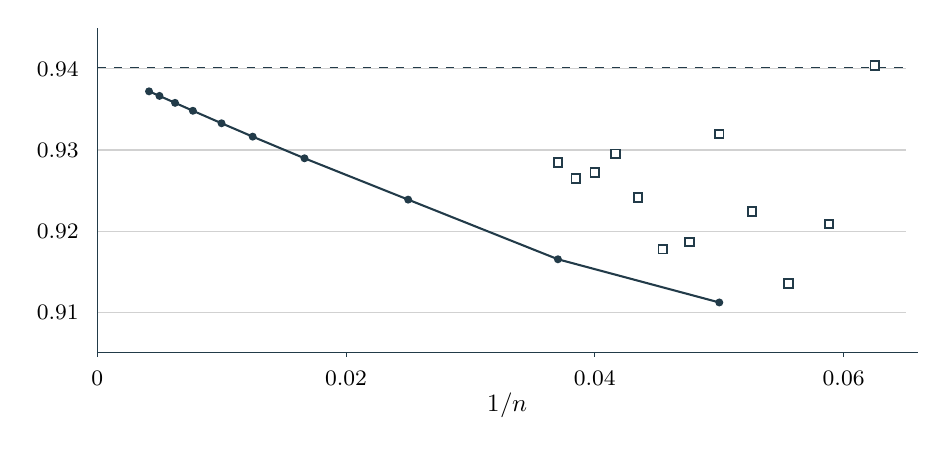
\begin{tikzpicture}[x=158cm,y=103cm]
 \begin{scope}[shift={(0,-.905)}]
 \foreach \v/\letra in {.910/{0.91},.920/{0.92},.930/{0.93},.940/{0.94}}{
   \draw[black!18] (0,\v)--(.065,\v);
   \node[anchor=east,font=\footnotesize] at (-.0007,\v) {\letra};}
 \draw[btinta] (0,.905)--(.066,.905) (0,.905)--(0,.945);
 \foreach \v/\letra in {0/{0},.02/{0.02},.04/{0.04},.06/{0.06}}{
   \draw[btinta] (\v,.905)--(\v,.9045);
   \node[anchor=north,font=\footnotesize] at (\v,.904) {\letra};}
 \draw[btinta,dashed] (0,.940144)--(.065,.940144);
 \draw[btinta,line width=.75pt] plot coordinates
{(0.050000000,0.911188472) (0.037037037,0.916522978) (0.025000000,0.923873790) (0.016666667,0.928966033)
(0.012500000,0.931643280) (0.010000000,0.933288384) (0.007692308,0.934831567) (0.006250000,0.935807595)
(0.005000000,0.936660345) (0.004166667,0.937232189)};
 \foreach \x/\y in {0.050000000/0.911188472,0.037037037/0.916522978,0.025000000/0.923873790,%
0.016666667/0.928966033,0.012500000/0.931643280,0.010000000/0.933288384,0.007692308/0.934831567,%
0.006250000/0.935807595,0.005000000/0.936660345,0.004166667/0.937232189}{\fill[btinta] (\x,%
\y) circle[radius=1.45pt];}
 \foreach \x/\y in {0.062500000/0.940434608,0.058823529/0.920874442,0.055555556/0.913509083,%
0.052631579/0.922429638,0.050000000/0.931979175,0.047619048/0.918660405,0.045454545/0.917777869,%
0.043478261/0.924122583,0.041666667/0.929528249,0.040000000/0.927235036,0.038461538/0.926480702,%
0.037037037/0.928458576}{\draw[btinta,fill=white,line width=.65pt]
    (\x,\y) ++(-1.55pt,-1.55pt) rectangle ++(3.1pt,3.1pt);}
 \node[anchor=north,font=\small] at (.033,.9012) {$1/n$};
 \end{scope}
\end{tikzpicture}
\caption{Centered terms with the same reference $\Phi_0$. The circles, joined by line segments,
represent the predictor in Table~\ref{tab:predictor}; the unconnected squares represent the exact count
in Table~\ref{tab:exacto}. The dashed horizontal line marks the value of the predictor constant
from the Nyström discretization. The sizes shown are those in the two tables.}
\label{fig:comparacion}
\end{figure}


At $n=20$ and $n=27$ we have $\log Q(n)-\log Q_{\rm pred}(n)=0.0208$ and $0.0119$. The two numbers
are compatible with a difference of order $1/n$, but they do not allow us to estimate its limit.

The programs and data used to obtain the numerical values in this section form the numerical verification
package
accompanying the paper~\cite{Codigo}.

\section{Discussion}\label{sec:discusion}

\paragraph{What remains open for the exact count.}
Set $R_Q(n)=\log Q(n)-\log Q_{\rm pred}(n)$. Theorem~\ref{thm:intro-constante} is equivalent to
\[
 \log Q(n)-\log n!-n\Phi=C_{\rm pred}+R_Q(n)+o(1).
\]
Thus $R_Q(n)\to0$ suffices for the constant term of $\log Q(n)$ to equal $C_{\rm pred}$. If
all that were known was that $R_Q(n)$ has a finite limit $r$, the constant term would exist and would equal
$C_{\rm pred}+r$. We have proved neither statement. The natural quantitative form is the following.

\begin{conjetura}\label{conj:RQ}
There exist $C$ and $n_0$ such that $|\log Q(n)-\log Q_{\rm pred}(n)|\le C/n$ for all $n\ge n_0$.
\end{conjetura}

Section~\ref{sec:numerico} gives $R_Q(20)\approx0.021$ and $R_Q(27)\approx0.012$.

\paragraph{The role of consistency.}
Theorem~\ref{thm:intro-consistencia} states that, on residual boards in its classes, the predictor satisfies
the exact recursion for the count at each step up to a factor $e^{O(k^{-2})}$. Along a trajectory of
residual boards that
stays in a single class with $k\ge\delta_0n$, the errors sum to $O_{\delta_0}(1/n)$
(Section~\ref{sec:B4T05}). To pass from this to $R_Q(n)\to0$ requires three ingredients that this paper
does not provide: membership of typical residual boards of a random placement in these classes; control of
the end of the process, when few empty rows remain (for the exact count,~\cite{Completabilidad} studies the
case of
a fixed number of queens left to place, without uniformity as this number grows); and a comparison between
the count and the predictor along random trajectories.

The comparison is exact at each step. Let $R(B)=\log Q(B)-L(B)$, so that $R_Q(n)$ is its value on
the full board (Lemma~\ref{lem:puente}), and let $\tilde w_c=e^{L(B+c)-L(B)}/\rho(B)$, which are positive
weights summing to one over the children of row $r$. If $Q(B)>0$ and the predictor is defined at $B$
and at these children, the recursion for the count gives
\[
 R(B)=\log\rho(B)+\log\sum_{c\in r}\tilde w_c\,e^{R(B+c)},
\]
where a child without completions contributes zero to the sum. This identity indicates what would have
to be controlled to bound $R_Q(n)$: the values of $\log\rho$ along the tree of insertions, averaged
with these weights, and the value of $R$ on the residual boards where the predictor ceases to be
defined.

\paragraph{Finite activity.}
The predictor is defined directly on the full board, on the polytope $K_n$. At finite
activity $\lambda$, the corresponding approximation uses the small branch of the Bethe equations.
For $n\ge6$, existence of the small branch for every $\lambda>0$ is a conjecture. A floating-point
calculation, without rigorous bounds, finds it at the 61 activities tested, spaced
logarithmically between $\Lambda=\lambda(n-1)=10^{-3}$ and $10^{12}$, for $n=6$, $7$, $8$, $10$, $12$,
$16$, $20$, $27$, $40$, $60$, $80$, $120$ and $160$. For $n=4$, $K_4$ reduces to the point
$\pi\equiv1/4$, because each row has four squares with $p_c\le1/4$ and sums to one; hence
$(H_\infty)$ does not hold. For $n=5$, the calculation indicates $\max_c\pi^{(5)}_c=1/4$. In both cases, a
barrier optimizer suggests that the branch ceases to exist for large $\Lambda$, but this has not been
proved.
Nothing in this paragraph is used in the rest of the paper.

% The bookmark anchor goes inside the title, so that the PDF bookmark leads to the title.
\section*{\phantomsection Use of artificial intelligence tools}
\addcontentsline{toc}{section}{Use of artificial intelligence tools}

Artificial intelligence tools were used to organize the sources, compare versions, prepare the typesetting
and editorial restructuring of the text, and conduct adversarial reviews of text excerpts.

\appendix
\section{A model case with rooks}\label{sec:torres}

In this appendix we study the construction of the predictor in the rook model, which has only
rows and columns. Everything is explicit in this setting, and one can prove that the Bethe formula
with the one-loop correction and the exact zero-mode normalization approximates the logarithm of the count with error $O(1/k)$,
uniformly from positive densities up to the full board. No proof in the rest of the paper
uses this appendix. We use separate notation here. In particular, $p$ is the Bethe square probability,
$\pi=3.14159\ldots$, and $D$ is a probability law.

\subsection{Definitions and theorem statement}

\paragraph{The model.}
Let $k\ge3$. On the $k\times k$ board, the lines are the $k$ rows and the $k$ columns. For
$\lambda>0$ we set
\[
 Z_k(\lambda)=\sum_{q=0}^{k}\binom kq^2q!\,\lambda^q,
\]
which is the sum of the weight $\lambda^q$ over all placements of nonattacking rooks, where $q$
is the number of rooks. To obtain
the coefficient, first choose the $q$ occupied rows and the $q$ occupied columns. Each
bijection between the two sets then places one rook in each chosen row and gives one of the $q!$
possible placements for this choice. Write $\Lambda=\lambda(k-1)$.

\paragraph{The uniform Bethe fixed point.}
The square probability $p\in(0,1/k)$ and the empty-line probability $y\in(0,1)$ satisfy
\begin{equation}\label{eq:torres-punto}
 p(1-p)=\lambda y^2,\qquad y=1-kp.
\end{equation}
This is the general equation $p_c(1-p_c)^{d-1}=\lambda\prod_{L\ni c}y_L$, with $y_L=1-\sum_{c\in L}p_c$
and $d$ the number of lines through each square, specialized to $d=2$ with all variables equal. Set $\theta=1-y=kp$, the Bethe mean number of rooks per row,
$w=p/(1-p)$, and $u=k\theta/(1-p)$.

\paragraph{The three components of the formula.}
At this fixed point we define
\begin{itemize}
\item the tree term
 \[
  \log Z_B=(\log\lambda)\sum_cp-\sum_Ly\log y-\sum_cp\log p+\sum_c(1-p)\log(1-p),
 \]
 where $c$ ranges over the $k^2$ squares and $L$ over the $2k$ lines,
\item the one-loop matrix $M$, acting on the $2k^2$ states $(c,f)$, with
 $f\in\{\text{row},\text{column}\}$. Its entries are $M[(c,f),(c',f')]=w$ if $f'\ne f$, $c'$ lies on the line of
 family $f'$ through $c$, and $c'\ne c$, and $M[(c,f),(c',f')]=0$ otherwise,
\item the zero-mode factor $\rho_0=\mathsf P/P_G$, where $\mathsf P=\mathbb P(N_R=N_C)$ for two
 independent variables $N_R$ and $N_C$ with law $\mathrm{Bin}(k,y)$, representing the auxiliary numbers of empty rows and
 columns in the Bethe model, and $P_G=(2\pi(V_R+V_C))^{-1/2}$, with $V_R=V_C=ky(1-y)$.
\end{itemize}
The formula and its remainder are
\begin{equation}\label{eq:torres-formula}
 F_k(\lambda)=\log Z_B-\tfrac12\log\det(I+M)+\log\rho_0,\qquad R'_k(\lambda)=\log Z_k(\lambda)-F_k(\lambda).
\end{equation}

\begin{teorema}[Rook model]\label{thm:torres}
The remainder $R'_k$ in~\eqref{eq:torres-formula} has the following properties.
\begin{enumerate}[(i)]
\item \emph{Uniform bound.} For each $\Lambda_0>0$ there is a constant $C=C(\Lambda_0)$ such that, for
 every $k\ge3$ and every $\lambda$ with $\Lambda=\lambda(k-1)\ge\Lambda_0$, we have $|R'_k(\lambda)|\le C/k$.
 Moreover, $R'_k(\lambda)$ has a limit $R'_k(\infty)$ as $\lambda\to\infty$, and the same bound holds
 for this limit.
\item \emph{Full board.}
 \[
 \begin{aligned}
  R'_k(\infty)={}&\log k!-k\log k-k(k-1)\log\bigl(1-\tfrac1k\bigr)
  +\tfrac12(k-1)^2\log\bigl(1-(k-1)^{-2}\bigr)\\
  &+\tfrac12\log\frac{2k}{k-1}+(k-1)\log\frac k{k-1}-\tfrac12\log(4\pi k),
 \end{aligned}
 \]
 and $R'_k(\infty)=-\frac1{12k}-\frac1{4k^2}+O(k^{-3})$.
\item \emph{The condition $\Lambda_0>0$ is necessary.} For each fixed $k$, $R'_k(\lambda)=-\frac12\log(4\pi k^2\lambda)+o(1)$
 as $\lambda\to0^+$. In particular, $R'_k$ is unbounded on $\lambda\in(0,\infty)$.
\end{enumerate}
\end{teorema}

The first three terms in (ii) equal $\log k!-\log\operatorname{perm}_B(J_k)$, where $J_k$ is the
$k\times k$ all-ones matrix and $\operatorname{perm}_B$ is the Bethe permanent~\cite{Vontobel}.

\begin{observacion}[Why $k\ge3$ is needed]
For $k=2$ the factors $1-(k-1)^2w^2$ and $(1-w^2)^{(k-1)^2}$ in Lemma~\ref{lem:torres-lazo} coincide, and
$\det(I+M)=(1-w^2)^2(1+w^2)^2$ vanishes like $y^2$ as $y\to0$. Then
$-\frac12\log\det(I+M)\sim-\log y$ is not canceled by the $\frac12\log y$ term in $\log\rho_0$, and $R'_2\to-\infty$
like $-\frac14\log\Lambda$. For $k\ge3$ only the factor $1-(k-1)^2w^2$ vanishes as $y\to0$. It vanishes
like $y$, and the cancellation is exact (Section~\ref{sec:torres-i}).
\end{observacion}

\begin{observacion}[The constant $C(\Lambda_0)$]
By (iii), for each fixed $k$, $\sup\{|R'_k(\lambda)|:\lambda(k-1)\ge\Lambda_0\}\to\infty$ as
$\Lambda_0\to0$, so $C(\Lambda_0)$ necessarily tends to infinity as $\Lambda_0\to0$. The proof of (i) gives an
explicit bound only for $k\ge k_2(\Lambda_0)$, with $k_2$ very large. For $3\le k<k_2$ the bound follows from a
compactness argument.
\end{observacion}

\paragraph{Idea of the proof.}
An exact identity (Lemma~\ref{lem:torres-identidad}) gives
$Z_k=Z_B\,(1-p)^{-k^2}\,\mathsf P\,\mathbb E_D[q!\,u^{-q}]$, where $\mathbb E_D$ denotes an average under the law
$D$ of the number of occupied rows conditional on $N_R=N_C$. The factor
$(1-p)^{-k^2}\approx e^{k\theta+\theta^2/2}$ is not negligible. In the full-board limit we
have $\mathsf P\to1$, and $D$ concentrates on $q=k$. After division by $\lambda^k$, the identity becomes
the all-ones case of the Watanabe--Chertkov formula~\cite{WC}, which expresses
the permanent of a nonnegative matrix as the product of its Bethe permanent, the permanent of
the matrix with entries $\beta_{ij}(1-\beta_{ij})$, and the factor $\prod_{i,j}(1-\beta_{ij})^{-1}$, where
$\beta$ is the doubly stochastic matrix at the Bethe fixed point. For the all-ones matrix,
$\beta_{ij}=1/k$, and these three factors are the limits of $Z_B/\lambda^k$,
$\mathbb E_D[q!\,u^{-q}]$, and $(1-p)^{-k^2}$. The discrete factor $\mathsf P$, which is the
zero mode, cancels exactly with its counterpart in the formula. What remains is $\mathbb E_D[q!\,u^{-q}]$, the average of a
slowly varying function. This average is evaluated by the one-dimensional Laplace method. The necessary
bounds follow from the fact that $D$ is a Poisson binomial law whose parameters come from the zeros of the
Legendre polynomials, and from Bruns's inequality.

\subsection{The uniform fixed point and closed forms}

\begin{lema}\label{lem:torres-punto}
For each $\lambda>0$ there is a unique $y\in(0,1)$ satisfying~\eqref{eq:torres-punto}. The map
$\lambda\mapsto y$ is a continuous decreasing bijection from $(0,\infty)$ onto $(0,1)$, with $y\to0$ as
$\lambda\to\infty$ and $y\to1$ as $\lambda\to0$. Moreover, $\Lambda\le\theta/y^2$. Hence
$\Lambda\ge\Lambda_0$ implies $\theta\ge\theta_0$, where $\theta_0\in(0,1)$ is the root of
$\theta_0=\Lambda_0(1-\theta_0)^2$.
\end{lema}
\begin{proof}
With $p=(1-y)/k$, equation~\eqref{eq:torres-punto} reads $\lambda=\varphi(y)$, with
$\varphi(y)=(1-y)(k-1+y)/(k^2y^2)$. The function $\varphi$ is smooth on $(0,1]$, tends to $\infty$ as
$y\to0^+$, and satisfies $\varphi(1)=0$. Let $\mathcal N(y)=(1-y)(k-1+y)=(k-1)-(k-2)y-y^2$. Then
$\varphi'(y)=(\mathcal N'(y)y-2\mathcal N(y))/(k^2y^3)$ and
\[
 \mathcal N'(y)y-2\mathcal N(y)=(k-2)y-2(k-1)<0\qquad\text{in }(0,1).
\]
Thus $\varphi$ is strictly decreasing, which gives the bijection and the limits. For the bound, we have
\[
 \Lambda=(k-1)\varphi(y)=\frac{\theta}{y^2}\cdot\frac{k-1}k\cdot\frac{k-1+y}k\le\frac\theta{y^2}.
\]
If $\Lambda\ge\Lambda_0$, then $\theta\ge\Lambda_0y^2=\Lambda_0(1-\theta)^2$. The function
$\theta\mapsto\theta-\Lambda_0(1-\theta)^2$ increases on $[0,1]$ from $-\Lambda_0$ to $1$. Hence
$\theta\ge\theta_0$.
\end{proof}

\begin{lema}[Tree term]\label{lem:torres-arbol}
At the uniform fixed point, $\log Z_B=-2k\log y+k^2\log(1-p)$.
\end{lema}
\begin{proof}
There are $k^2$ squares and $2k$ lines, and $\sum_cp=k^2p=k\theta$. Hence
\[
 \log Z_B=k\theta\log\lambda-2ky\log y-k^2p\log p+k^2(1-p)\log(1-p).
\]
By~\eqref{eq:torres-punto}, $\log\lambda=\log p+\log(1-p)-2\log y$. On substitution, the term
$k\theta\log p$ cancels with $-k^2p\log p$, leaving
$\log Z_B=-2k(\theta+y)\log y+(k\theta+k^2-k^2p)\log(1-p)$. Since $\theta+y=1$ and $k^2p=k\theta$, this equals
$-2k\log y+k^2\log(1-p)$.
\end{proof}

\begin{lema}[One-loop correction]\label{lem:torres-lazo}
We have
\[
 \det(I+M)=\bigl(1-(k-1)^2w^2\bigr)\bigl(1+(k-1)w^2\bigr)^{2(k-1)}\bigl(1-w^2\bigr)^{(k-1)^2}
\]
and $1-(k-1)^2w^2=y\,(1+(k-2)p)/(1-p)^2$. For $k\ge3$, all factors are positive when
$y\in(0,1)$.
\end{lema}
\begin{proof}
Order the states in two blocks, $(c,\text{row})$ and $(c,\text{column})$. Within each block,
the squares $c=(i,j)$ are in Kronecker order, with $i$ the outer index and $j$ the inner index. Let $J$ denote the
$k\times k$ all-ones matrix. From $(c,\text{row})$ the next family is the column family, so $c'=(i',j)$ with
$i'\ne i$. This gives the row-to-column block $wE$, with $E=(J-I)\otimes I$. From
$(c,\text{column})$ the transition is to $c'=(i,j')$ with $j'\ne j$, giving the block $wE'$, with
$E'=I\otimes(J-I)$. The diagonal blocks vanish because $f'\ne f$. Thus the Schur complement gives
\[
 I+M=\begin{pmatrix}I&wE\\ wE'&I\end{pmatrix},\qquad \det(I+M)=\det(I-w^2E'E),
\]
and $E'E=(J-I)\otimes(J-I)$. The matrix $J-I$ is symmetric, with eigenvalues $k-1$ (once) and $-1$ ($k-1$
times). The eigenvalues of the Kronecker product are the pairwise products, namely $(k-1)^2$ (once), $-(k-1)$
($2(k-1)$ times), and $1$ ($(k-1)^2$ times). This gives the formula. For the second identity, we have
\[
 1-(k-1)^2w^2=\frac{\bigl[(1-p)-(k-1)p\bigr]\bigl[(1-p)+(k-1)p\bigr]}{(1-p)^2}
 =\frac{(1-kp)(1+(k-2)p)}{(1-p)^2}.
\]
For positivity, $p=\theta/k\le1/k$, so $w\le1/(k-1)\le\frac12$ if $k\ge3$. Hence
$1-w^2\ge\frac34$, and the first factor is proportional to $y>0$.
\end{proof}

\begin{lema}[Zero mode]\label{lem:torres-cero}
Let $\beta(q)=\binom kq\theta^qy^{k-q}$ denote the $\mathrm{Bin}(k,\theta)$ law of the number of occupied rows.
Then $\mathsf P=\sum_{q=0}^k\beta(q)^2$ and $\log\rho_0=\log\mathsf P+\frac12\log(4\pi ky\theta)$.
\end{lema}
\begin{proof}
The equality $N_R=N_C$ is equivalent to $k-N_R=k-N_C$, and $k-N_R$ has law $\mathrm{Bin}(k,\theta)$. Moreover,
$V_R+V_C=2ky\theta$.
\end{proof}

\subsection{The exact identity}

\begin{lema}\label{lem:torres-identidad}
For every $\lambda>0$, with $y=y(\lambda)$,
\[
 Z_k(\lambda)=y^{-2k}\sum_{q=0}^k\beta(q)^2q!\,u^{-q}.
\]
Let $D$ be the probability law $D(q)=\beta(q)^2/\mathsf P$ on $\{0,\dots,k\}$. Then
\begin{equation}\label{eq:torres-identidad}
 R'_k(\lambda)=\log\mathbb E_D[q!\,u^{-q}]-k^2\log(1-p)+\tfrac12\log\det(I+M)-\tfrac12\log(4\pi ky\theta).
\end{equation}
\end{lema}
\begin{proof}
Since $\binom kq^2=\beta(q)^2\theta^{-2q}y^{-2(k-q)}$, we have
$Z_k=y^{-2k}\sum_q\beta(q)^2q!\,(\lambda y^2/\theta^2)^q$. By~\eqref{eq:torres-punto} and $p=\theta/k$,
$\lambda y^2/\theta^2=p(1-p)/\theta^2=(1-p)/(k\theta)=1/u$, giving the first formula. Hence
$\log Z_k=-2k\log y+\log\mathsf P+\log\mathbb E_D[q!\,u^{-q}]$. Subtracting $F_k$, expressed using
Lemmas~\ref{lem:torres-arbol} and~\ref{lem:torres-cero}, cancels the terms $-2k\log y$ and $\log\mathsf P$
exactly and leaves~\eqref{eq:torres-identidad}.
\end{proof}

Thus the entire discrete part of the zero mode, the exact probability of $N_R=N_C$, appears identically in
$Z_k$ and in the formula. What remains is the average under $D$ of $q!\,u^{-q}$, a slowly varying
function whose logarithm has second difference $\log((q+1)/q)$, of order $1/q$.

\subsection{The law \texorpdfstring{$D$}{D} and its moments}

\begin{lema}[Legendre]\label{lem:torres-legendre}
Let $\cos\alpha_1>\dots>\cos\alpha_k$ be the zeros of the Legendre polynomial $P_k$, with
$0<\alpha_1<\dots<\alpha_k<\pi$. Then, for every $x$,
\[
 f_k(x):=\sum_{q=0}^k\binom kq^2x^q=\prod_{i=1}^k(1+xc_i),\qquad c_i=\cot^2(\alpha_i/2)>0.
\]
\end{lema}
\begin{proof}
By Rodrigues' formula, $P_k(t)=(2^kk!)^{-1}(d/dt)^k[(t-1)^k(t+1)^k]$, and by the Leibniz rule
\[
 \Bigl(\frac{d}{dt}\Bigr)^k\bigl[(t-1)^k(t+1)^k\bigr]
 =\sum_q\binom kq\frac{k!}{q!}(t-1)^q\,\frac{k!}{(k-q)!}(t+1)^{k-q}.
\]
Hence $P_k(t)=\sum_q\binom kq^2\bigl(\frac{t-1}2\bigr)^q\bigl(\frac{t+1}2\bigr)^{k-q}$. For $x\ne1$, let
$t=(1+x)/(1-x)$. Then $(t-1)/2=x/(1-x)$ and $(t+1)/2=1/(1-x)$, giving
$f_k(x)=(1-x)^kP_k\bigl((1+x)/(1-x)\bigr)$. Both sides are polynomials in $x$, so the identity holds
for every $x$. The polynomial $P_k$ has $k$ simple zeros $t_i=\cos\alpha_i$ in
$(-1,1)$~\cite[Theorem~3.3.1]{Szego}. If
$\kappa_k$ is its leading coefficient, then $f_k(x)=\kappa_k\prod_i[(1-t_i)+x(1+t_i)]$. Since $f_k(0)=1$, we
have $\kappa_k\prod_i(1-t_i)=1$. Using $(1+\cos\alpha)/(1-\cos\alpha)=\cot^2(\alpha/2)$ gives the product
in the statement.
\end{proof}

\begin{corolario}\label{cor:torres-pb}
Let $x=(\theta/y)^2$, so that $D(q)=\binom kq^2x^q/f_k(x)$.
\begin{enumerate}[(a)]
\item The generating function is $\mathbb E_D[\tau^q]=f_k(x\tau)/f_k(x)=\prod_i(1-r_i+r_i\tau)$, with
 $r_i=xc_i/(1+xc_i)\in(0,1)$. Thus $D$ is the law of a sum of $k$ independent Bernoulli
 variables with parameters $r_i$ (see~\cite{Pitman} on this representation).
\item For $v\in\mathbb R$, the tilted law $D_v(q)\propto D(q)e^{vq}$ is in the same family, with $x$
 replaced by $xe^v$.
\item The function $K(v)=\log\mathbb E_D[e^{vq}]=\sum_i\log(1-r_i+r_ie^v)$ satisfies
 \[
 \begin{aligned}
  K'(v)&=\sum_ir_i(v)=:\mu(v),\qquad K''(v)=\sum_ir_i(v)(1-r_i(v))=:\sigma^2(v),\\
  K'''(v)&=\sum_ir_i(v)(1-r_i(v))(1-2r_i(v)),\\
  K''''(v)&=\sum_ir_i(v)(1-r_i(v))\bigl(1-6r_i(v)(1-r_i(v))\bigr),
 \end{aligned}
 \]
 with $r_i(v)=r_ie^v/(1-r_i+r_ie^v)$.
\item Consequently, $|K'''|\le K''$, $|K''''|\le K''$, $0\le K''\le k/4$,
 $K''(0)e^{-|v|}\le K''(v)\le K''(0)e^{|v|}$, and $K(v)\le0$ for $v\le0$.
\end{enumerate}
\end{corolario}
\begin{proof}
Part (a) follows from Lemma~\ref{lem:torres-legendre}, and (b) from $\binom kq^2(xe^v)^q\propto D(q)e^{vq}$.
The
derivatives in (c) are those of a sum of logarithms of Bernoulli generating functions. The
inequalities $|1-2r|\le1$ and $|1-6r(1-r)|\le1$ give the first two bounds in (d), and $r(1-r)\le\frac14$
gives
$K''\le k/4$. For the fourth bound it suffices to use $|(\log K'')'|=|K'''/K''|\le1$. Finally, $K(v)\le0$
for $v\le0$
because $q\ge0$.
\end{proof}

\begin{lema}\label{lem:torres-momentos}
Let $x>0$, $s=\sqrt x$, $\theta_x=s/(1+s)$, and $y_x=1-\theta_x$, and let $\mu_D$ and $\sigma_D^2$ be the
mean and
variance of the law $q\mapsto\binom kq^2x^q/f_k(x)$. Then
\[
 \bigl|\mu_D-(k+\tfrac12)\theta_x\bigr|\le1,\qquad \bigl|\sigma_D^2-(k+\tfrac12)\theta_xy_x/2\bigr|\le1.
\]
With $x=(\theta/y)^2$ the law is $D$ and we have $\theta_x=\theta$ and $y_x=y$. By
Corollary~\ref{cor:torres-pb}(b), for the tilted law $D_v$, whose mean is $\mu(v)$ and whose variance is
$\sigma^2(v)$, it suffices to set $s_v=se^{v/2}$, $\theta_v=s_v/(1+s_v)$, and $y_v=1-\theta_v$.
\end{lema}
\begin{proof}
By Corollary~\ref{cor:torres-pb}, $\mu_D=\sum_iF(\alpha_i)$ and $\sigma_D^2=\sum_iG(\alpha_i)$, with
$F(\alpha)=s^2/(s^2+\tan^2(\alpha/2))$ and $G=F(1-F)$. The function $F$ is continuous and decreases on
$[0,\pi]$ from $1$ to $0$. The function $G$ takes values in $[0,\frac14]$, vanishes at the endpoints, and is
unimodal. It increases while $F>\frac12$ and decreases while $F<\frac12$. By Bruns's
inequality~\cite{Bruns} (see also~\cite[\S6.21]{Szego}), with $h=\pi/(k+\frac12)$,
\[
 (i-\tfrac12)h\le\alpha_i\le ih\qquad(i=1,\dots,k).
\]
By Lemma~\ref{lem:torres-riemann}, proved below, with $m_0=1$ for $F$ and
$m_0=\frac14$ for $G$, each sum differs from the corresponding $h^{-1}\int_0^\pi$ by at most $1$. With
$t=\tan(\alpha/2)$ and
$d\alpha=2\,dt/(1+t^2)$, we obtain
\[
\begin{aligned}
 \int_0^\pi F\,d\alpha&=2\int_0^\infty\frac{s^2\,dt}{(t^2+s^2)(1+t^2)}=\frac{\pi s}{1+s}=\pi\theta_x,\\
 \int_0^\pi G\,d\alpha&=2\int_0^\infty\frac{s^2t^2\,dt}{(t^2+s^2)^2(1+t^2)}=\frac{\pi s}{2(1+s)^2}
 =\frac\pi2\,\theta_xy_x;
\end{aligned}
\]
Both integrals follow by partial fractions (at $s=1$, by continuity). Since $h^{-1}=(k+\frac12)/\pi$, this
gives
the stated bounds.
\end{proof}

\begin{lema}[Riemann sums at interlaced points]\label{lem:torres-riemann}
Let $h=\pi/(k+\frac12)$, $\alpha_i\in[(i-\frac12)h,ih]$ for $i=1,\dots,k$, and $m_0>0$.
\begin{enumerate}[(a)]
\item If $F:[0,\pi]\to[0,m_0]$ is nonincreasing, then
 $\bigl|\sum_iF(\alpha_i)-h^{-1}\int_0^\pi F\bigr|\le m_0$.
\item If $G:[0,\pi]\to[0,m_0]$ is unimodal, then
 $\bigl|\sum_iG(\alpha_i)-h^{-1}\int_0^\pi G\bigr|\le4m_0$.
\end{enumerate}
\end{lema}
\begin{proof}
(a) Extend $F$ by $0$ outside $[0,\pi]$. It remains nonincreasing on $[0,\infty)$. First,
$F(\alpha_i)\le F((i-\frac12)h)$, whose right-hand side for $i\ge2$ is at most
$h^{-1}\int_{(i-3/2)h}^{(i-1/2)h}F$ and for
$i=1$ is at most $m_0$. Hence $\sum_iF(\alpha_i)\le m_0+h^{-1}\int_0^\pi F$. Conversely,
$F(\alpha_i)\ge F(ih)\ge h^{-1}\int_{ih}^{(i+1)h}F$. Since $(k+1)h\ge\pi$, we have
$\sum_iF(\alpha_i)\ge h^{-1}\int_h^\pi F\ge h^{-1}\int_0^\pi F-m_0$.

(b) Set $I_i=[(i-1)h,ih]$. Since $\alpha_i\in I_i$,
\[
 \left|G(\alpha_i)-h^{-1}\int_{I_i}G\right|
 \le\operatorname{osc}_{I_i}G .
\]
By unimodality and $0\le G\le m_0$, the sum of the oscillations over these intervals
is at most the total variation of $G$ on $[0,kh]$, which is at most $2m_0$.
Since $\pi-kh=h/2$, the remainder $h^{-1}\int_{kh}^{\pi}G$ contributes at most $m_0/2$.
The triangle inequality gives the bound $5m_0/2\le4m_0$, including when the mode is at an endpoint.
\end{proof}

\subsection{The Laplace step}

Since $q!=\int_0^\infty e^{-t}t^q\,dt$, Tonelli's theorem gives
$\mathbb E_D[q!\,u^{-q}]=\int_0^\infty e^{-t}\,\mathbb E_D[(t/u)^q]\,dt$. With $t=ue^v$ this becomes
\begin{equation}\label{eq:torres-laplace}
 \mathbb E_D[q!\,u^{-q}]=u\int_{\mathbb R}e^{\Psi(v)}\,dv,\qquad \Psi(v)=-ue^v+v+K(v),
\end{equation}
with $\Psi(0)=-u$, $\Psi'(0)=1+\mu_D-u$, and $\Psi''(0)=-(u-\sigma_D^2)$.

\begin{lema}\label{lem:torres-psi}
Suppose $\theta\in[\theta_0,1)$, that is, $\lambda<\infty$, so that $x=(\theta/y)^2$ is finite, and assume
$k\ge k_1:=\max(11,20/\theta_0)$. Let $\delta=0.3$. Then
\begin{enumerate}[(a)]
\item $\Psi''(v)\le-a$ for every $v\ge-\delta$, with $a=0.08\,k\theta_0$,
\item $\Psi'(v)>0$ for every $v\le-\delta$, and $\Psi(v)\le v$ for every $v\le0$,
\item $|\Psi'''(v)|\le b$ and $|\Psi''''(v)|\le b$ for $|v|\le\delta$, with $b=2k$,
\item $|\Psi'(0)|\le4.5$ and $k\theta(1+\theta)/2-3.1\le u-\sigma_D^2\le k\theta(1+\theta)/2+3.1$.
\end{enumerate}
\end{lema}
\begin{proof}
(a) We have $\Psi''(v)=-ue^v+\sigma^2(v)$ and, by Lemma~\ref{lem:torres-momentos} applied to $D_v$,
$\sigma^2(v)\le(k+\frac12)\theta_vy_v/2+1$, with $\theta_vy_v=s_v/(1+s_v)^2$. Since $u\ge k\theta=ks/(1+s)$,
\[
 -\Psi''(v)\ge k\,se^{v/2}\Bigl[\frac{e^{v/2}}{1+s}-\frac1{2(1+se^{v/2})^2}\Bigr]-\frac1{16}-1.
\]
For $v\ge-\delta$, we have $1+se^{v/2}\ge e^{-\delta/2}(1+s)$, so the expression in brackets is at least
$(e^{-\delta/2}-e^\delta/2)/(1+s)>\gamma/(1+s)$, with $\gamma=0.1857$. Hence
$-\Psi''(v)\ge\gamma e^{-\delta/2}k\theta-1.07\ge0.159\,k\theta-1.07\ge0.08\,k\theta_0$ if
$k\theta_0\ge14$.

(b) By Lemma~\ref{lem:torres-momentos}, $\Psi'(v)=-ue^v+1+\mu(v)\ge(k+\frac12)\theta_v-ue^v$. For
$v\le0$, we have $\theta_v\ge se^{v/2}/(1+s)=\theta e^{v/2}$ and $u\le k\theta/(1-1/k)$. Hence
$\Psi'(v)\ge k\theta e^{v/2}\bigl[1-e^{v/2}/(1-1/k)\bigr]>0$ for $v\le-\delta$, since
$e^{-\delta/2}<0.861<1-1/k$ when $k\ge8$. Moreover, $\Psi(v)\le v$ for $v\le0$, since $-ue^v<0$ and
$K(v)\le0$.

(c) We have $\Psi'''=-ue^v+K'''$ and $\Psi''''=-ue^v+K''''$. Since $|K'''|,|K''''|\le k/4$ and
$ue^v\le1.1k\,e^{0.3}\le1.5k$ for $k\ge11$, both absolute values are at most $1.75k\le b$.

(d) By Lemma~\ref{lem:torres-momentos}, $|\mu_D-k\theta|\le1+\theta/2\le\frac32$ and
$u-k\theta=\theta^2/(1-p)\in[0,2]$. Since $\Psi'(0)=1+(\mu_D-k\theta)-(u-k\theta)$, we obtain
$|\Psi'(0)|\le4.5$. For $u-\sigma_D^2$ we also use $|\sigma_D^2-(k+\frac12)\theta y/2|\le1$ and
$1-y/2=(1+\theta)/2$.
\end{proof}

\begin{lema}[Laplace's method with an explicit error bound]\label{lem:torres-laplace}
Let $\Psi\in C^4(\mathbb R)$ and let the constants $a,b>0$, $\delta\in(0,1]$, $r\in(0,\delta/2]$ with
$r\le1$ and
$br\le a$, and $V\ge0$ satisfy the following conditions.
\begin{enumerate}[label=(L\arabic*)]
\item $\Psi''\le-a$ on $[-\delta,\infty)$.
\item $\Psi'>0$ on $(-\infty,-\delta]$, and $\Psi(v)\le v$ for $v\le-\delta$.
\item $|\Psi'''|\le b$ and $|\Psi''''|\le b$ on $[-\delta,\delta]$.
\item There exists $v^*$ with $|v^*|\le\delta/2$ and $\Psi'(v^*)=0$.
\item $\Psi(v^*)\ge-V$.
\end{enumerate}
Then $v^*$ is the global maximizer of $\Psi$ and, with $A=-\Psi''(v^*)\ge a$,
$\int_{\mathbb R}e^{\Psi}=e^{\Psi(v^*)}\sqrt{2\pi/A}\,(1+\varepsilon)$, where
\[
 |\varepsilon|\le\frac b{8A^2}+\frac{6b^2}{A^3}+\frac{e^{-Ar^2/2}}{r\sqrt A}
 +\sqrt A\Bigl[\frac{2e^{-ar^2/2}}{ar}+\Bigl(1+V+\frac{a\delta^2}8\Bigr)e^{-a\delta^2/8}\Bigr].
\]
\end{lema}
\begin{proof}
\emph{Global maximum.} By (L1) and (L2), $\Psi$ is increasing on $(-\infty,-\delta]$ and strictly concave on
$[-\delta,\infty)$, so $v^*$ is the global maximizer.

\emph{Central region $|t|\le r$, with $t=v-v^*$.} Taylor's theorem gives
$\Psi(v^*+t)=\Psi(v^*)-At^2/2+S(t)$, with
$S(t)=\Psi'''(v^*)t^3/6+T(t)$ and $|T(t)|\le bt^4/24$. Since $|t|\le r\le1$,
$|S|\le b|t|^3/4\le(br/4)t^2\le(A/4)t^2$. Write $e^S=1+S+R_2$, with $|R_2|\le S^2e^{|S|}/2$. The cubic
term integrates to zero on $[-r,r]$, and
\[
 \Bigl|\int e^{-At^2/2}\,T\Bigr|\le\frac b{24}\,3\sqrt{2\pi}\,A^{-5/2}=\sqrt{\frac{2\pi}A}\,\frac b{8A^2},
\]
\[
 \Bigl|\int e^{-At^2/2}R_2\Bigr|\le\frac{b^2}{32}\int t^6e^{-At^2/4}\,dt
 =\sqrt{\frac{2\pi}A}\,\frac{15\cdot2^{7/2}}{32}\,\frac{b^2}{A^3}\le\sqrt{\frac{2\pi}A}\,\frac{6b^2}{A^3}.
\]
Truncating the Gaussian on $|t|>r$ incurs an error of at most $2e^{-Ar^2/2}/(Ar)$, that is, a relative error
of at
most $e^{-Ar^2/2}/(r\sqrt A)$.

\emph{Parts of $[-\delta,\infty)$ outside the central region.} By concavity (L1), for $v\ge v^*+r$,
$\Psi(v)\le\Psi(v^*)-ar^2/2-ar(v-v^*-r)$, and the analogous bound holds on $[-\delta,v^*-r]$. Their
contribution is at
most $2e^{\Psi(v^*)-ar^2/2}/(ar)$.

\emph{Tail $(-\infty,-\delta]$.} Let $V'=V+a\delta^2/8$. If $V'<\delta$, there is no need to split the
integral,
since (L2) gives $\int_{-\infty}^{-\delta}e^\Psi\le\int_{-\infty}^{-\delta}e^v\,dv=e^{-\delta}\le e^{-V'}$.
Now suppose $V'\ge\delta$, as is the case in Proposition~\ref{prop:torres-laplace}, where
$V'\ge u\ge k\theta_0>375$. By (L2) and (L5), $\int_{-\infty}^{-V'}e^\Psi\le e^{-V'}\le
e^{\Psi(v^*)-a\delta^2/8}$.
Since $\Psi$ is increasing on $[-V',-\delta]$, we have $\int_{-V'}^{-\delta}e^\Psi\le V'e^{\Psi(-\delta)}$,
and by
concavity and $|v^*|\le\delta/2$, we have $\Psi(-\delta)\le\Psi(v^*)-a\delta^2/8$.

Dividing by $e^{\Psi(v^*)}\sqrt{2\pi/A}$ and using $(2\pi)^{-1/2}\le1$ gives the bound.
\end{proof}

\begin{proposicion}\label{prop:torres-laplace}
For each $\theta_0\in(0,1]$ there exist $k_2(\theta_0)$ and $C_1(\theta_0)$ such that, if
$\theta\in[\theta_0,1)$ and
$k\ge k_2$,
\[
 \log\mathbb E_D[q!\,u^{-q}]=\log u-u+\tfrac12\log(2\pi)-\tfrac12\log(u-\sigma_D^2)+\varepsilon',\qquad
 |\varepsilon'|\le C_1/k.
\]
\end{proposicion}
\begin{proof}
\emph{Hypotheses of Lemma~\ref{lem:torres-laplace}.} Take $\delta=0.3$, $a=0.08\,k\theta_0$, $b=2k$,
$r=a/b=0.04\,\theta_0$, and $V=u$. Hypotheses (L1)--(L3) hold by Lemma~\ref{lem:torres-psi}, and
(L5) holds because $\Psi(v^*)\ge\Psi(0)=-u$. For (L4), $\Psi'$ is strictly decreasing on
$[-\delta,\infty)$, with slope at most $-a$. Hence $\Psi'(\delta/2)\le\Psi'(0)-a\delta/2$ and
$\Psi'(-\delta/2)\ge\Psi'(0)+a\delta/2$. Since $|\Psi'(0)|\le4.5<a\delta/2$ if $k\theta_0>375$, the first
derivative value is negative and the second positive. Thus there is a unique $v^*$ with $\Psi'(v^*)=0$, and
$|v^*|\le|\Psi'(0)|/a\le4.5/a\le\delta/2$.

\emph{Size of the error.} Since $K''\ge0$ and $|v^*|\le\delta/2$,
we have $A=ue^{v^*}-K''(v^*)\le ue^{\delta/2}\le1.1\,e^{0.15}k\le1.28k$. Together with $A\ge a$ this gives
$a\le A\le1.28k$. The first two terms of the bound on $|\varepsilon|$ are $O(1/k)$,
since $b/(8A^2)\le2k/(8a^2)$ and $6b^2/A^3\le6b^2/a^3=46875/(\theta_0^3k)$. With $\theta_0$ fixed, $r$ is
constant,
$V=O(k)$, and $A$ is of order $k$. Hence the tail terms are
$O_{\theta_0}(k^{3/2}e^{-c(\theta_0)k})$, with $c(\theta_0)>0$. Taking $0<c'<c(\theta_0)$ absorbs the
prefactor into $O_{\theta_0}(e^{-c'k})$. Summing the two algebraic terms and the tails shows that there is a
$k_2(\theta_0)$ such that $|\varepsilon|\le1/2$ for $k\ge k_2$. Then
$|\log(1+\varepsilon)|\le2|\varepsilon|$.

\emph{Value at the maximum.} Taylor's theorem at $0$ with $\Psi''\le-a$ gives
$\Psi(v^*)\le\Psi(0)+\Psi'(0)v^*-av^{*2}/2\le\Psi(0)+\Psi'(0)^2/(2a)$. Hence
$0\le\Psi(v^*)-\Psi(0)\le\Psi'(0)^2/(2a)\le10.2/a=O(1/k)$.

\emph{Curvature.} Since $A=ue^{v^*}-K''(v^*)$,
\[
 |A-(u-\sigma_D^2)|\le
ue^{\delta}|v^*|+\sigma_D^2\bigl(e^{|v^*|}-1\bigr)\le1.35\,(u+\sigma_D^2)\cdot4.5/a=O(1),
\]
because $u+\sigma_D^2\le1.35k$. Since $u-\sigma_D^2\ge k\theta_0/2-3.1$, we have
$|\log A-\log(u-\sigma_D^2)|=O(1/k)$.

\emph{Conclusion.} By~\eqref{eq:torres-laplace},
$\log\mathbb E_D[q!\,u^{-q}]=\log u+\Psi(v^*)+\frac12\log(2\pi/A)+\log(1+\varepsilon)$, which gives the
claim.
\end{proof}

The threshold $k\ge93750/\theta_0^3$ ensures that $46875/(\theta_0^3k)\le1/2$. To bound $|\varepsilon|$ by
$1/2$,
we choose $k_2$ using the full sum. The constant $C(\Lambda_0)$ in Theorem~\ref{thm:torres}(i)
also requires a compactness argument for $3\le k<k_2$.

\subsection{Proof of Theorem~\ref{thm:torres}}\label{sec:torres-i}

\paragraph{Part (i).}
Let $\Lambda_0\le\Lambda<\infty$, so that $\theta\in[\theta_0,1)$ by Lemma~\ref{lem:torres-punto}. We treat
the
case $\lambda=\infty$ at the end by taking the limit. In~\eqref{eq:torres-identidad} we substitute the
expressions from
Proposition~\ref{prop:torres-laplace} and Lemma~\ref{lem:torres-lazo}. The term $\frac12\log y$ in
Lemma~\ref{lem:torres-lazo} cancels with the $-\frac12\log y$ term in $-\frac12\log(4\pi ky\theta)$. This is
the
zero-mode cancellation. Using $\log u=\log(k\theta)-\log(1-p)$ and
Lemma~\ref{lem:torres-psi}(d) to obtain $\log(u-\sigma_D^2)=\log(k\theta(1+\theta)/2)+O(1/k)$, we are left
with
\[
\begin{aligned}
 R'_k={}&-u-2\log(1-p)-k^2\log(1-p)-\tfrac12\log(1+\theta)+\tfrac12(k-1)^2\log(1-w^2)\\
 &+\tfrac12\log(1+(k-2)p)+(k-1)\log(1+(k-1)w^2)+O(1/k).
\end{aligned}
\]
We expand using $p=\theta/k\le1/k$, $w\le1/(k-1)\le\frac12$, and $k\ge3$. All the bounds are
uniform in $\theta\in[0,1]$.
\begin{enumerate}[(a)]
\item $-k^2\log(1-p)=k\theta+\theta^2/2+e_1$, with $0\le e_1\le\frac23k^2p^3\le\frac2{3k}$.
\item $-u=-k\theta-\theta^2/(1-p)=-k\theta-\theta^2-e_2$, with $0\le e_2=\theta^2p/(1-p)\le2/k$.
\item $0\le-2\log(1-p)\le2p/(1-p)\le4/k$.
\item $\frac12(k-1)^2\log(1-w^2)=-\theta^2/2+e_4$, with $|e_4|\le2/k$. Indeed, if
 $\zeta=(1-1/k)/(1-\theta/k)\in[1-1/k,1]$, then $(k-1)^2w^2=\theta^2\zeta^2$ and
 $|\theta^2\zeta^2-\theta^2|\le2/k$. Moreover, $0\le-\log(1-w^2)-w^2\le\frac43w^4$ and
$(k-1)^2w^4\le(k-1)^{-2}$.
\item $1+(k-2)p=1+\theta-2\theta/k$, and
 $\bigl|\frac12\log(1+\theta-2\theta/k)-\frac12\log(1+\theta)\bigr|\le\theta/k\le1/k$.
\item $(k-1)\log(1+(k-1)w^2)=\theta^2+e_6$, with $|e_6|\le3/k$. Here we use $0\le z-\log(1+z)\le z^2/2$ with
 $z=(k-1)w^2\le1/(k-1)$ and the same argument as in (d).
\end{enumerate}
On summing, the terms of order $k$ cancel ($k\theta-k\theta$), as do the terms of order one, since
\[
 -\theta^2+\tfrac12\theta^2-\tfrac12\log(1+\theta)-\tfrac12\theta^2+\tfrac12\log(1+\theta)+\theta^2=0.
\]
Hence $|R'_k|\le C(\theta_0)/k$ for $k\ge k_2(\theta_0)$.

For $3\le k<k_2$, $R'_k$ is continuous on $\lambda\in[\Lambda_0/(k-1),\infty)$, since all the components are
continuous functions of $y\in(0,1)$ and $\lambda\mapsto y$ is continuous. It has a finite limit as
$\lambda\to\infty$ (see the next paragraph, where finiteness follows from $k\ge3$). It is therefore bounded,
and since
there are only finitely many such $k$, it suffices to take $C\ge\max_{3\le k<k_2}k\sup|R'_k|$.

In the limit $\lambda\to\infty$, the only term of~\eqref{eq:torres-identidad} that is singular as
$y\to0$ is $\frac12\log y$, and it cancels identically. The other terms are continuous up to $y=0$, where
$D$ is the
unit point mass at $q=k$. The uniform bound passes to the limit.

\paragraph{Part (ii).}
As $\lambda\to\infty$, we have $y\to0$, $\theta\to1$, $p\to1/k$, $w\to1/(k-1)$, and $u\to k^2/(k-1)$, and
$D$
tends to the unit point mass at $q=k$, since $r_i\to1$ as $x\to\infty$. In~\eqref{eq:torres-identidad},
after
cancellation of $\frac12\log y$, we are left with
\[
\begin{aligned}
 R'_k(\infty)={}&\log k!-k\log\frac{k^2}{k-1}-k^2\log\bigl(1-\tfrac1k\bigr)
 +\tfrac12(k-1)^2\log\bigl(1-(k-1)^{-2}\bigr)\\
 &+\tfrac12\log\Bigl(1+\frac{k-2}k\Bigr)-\log\bigl(1-\tfrac1k\bigr)
 +(k-1)\log\Bigl(1+\frac1{k-1}\Bigr)-\tfrac12\log(4\pi k).
\end{aligned}
\]
Since $-k\log(k^2/(k-1))-k^2\log(1-1/k)=-k\log k-k(k-1)\log(1-1/k)$ and
$\frac12\log((2k-2)/k)-\log((k-1)/k)=\frac12\log(2k/(k-1))$, this gives the stated expression. For the
expansion we use Stirling's formula, which has no term of order $k^{-2}$, together with the expansions
below.
\[
\begin{aligned}
 \log k!&=k\log k-k+\tfrac12\log(2\pi k)+\tfrac1{12k}+O(k^{-3}),\\
 -k(k-1)\log\bigl(1-\tfrac1k\bigr)&=(k-1)\sum_{m\ge1}\frac1{m\,k^{m-1}}
 =k-\tfrac12-\tfrac1{6k}-\tfrac1{12k^2}+O(k^{-3}),\\
 \tfrac12(k-1)^2\log\bigl(1-(k-1)^{-2}\bigr)&=-\tfrac12-\tfrac1{4(k-1)^2}+O(k^{-4})
 =-\tfrac12-\tfrac1{4k^2}+O(k^{-3}),\\
 \tfrac12\log\frac{2k}{k-1}&=\tfrac12\log2+\tfrac1{2k}+\tfrac1{4k^2}+O(k^{-3}),\\
 (k-1)\log\frac k{k-1}&=1-\tfrac1{2k}-\tfrac1{6k^2}+O(k^{-3}).
\end{aligned}
\]
On summing, we have $\frac12\log(2\pi k)+\frac12\log2-\frac12\log(4\pi k)=0$ and $-\frac12-\frac12+1=0$. The
coefficient
of $1/k$ is $\frac1{12}-\frac16+\frac12-\frac12=-\frac1{12}$, and that of $1/k^2$ is
$-\frac1{12}-\frac14+\frac14-\frac16=-\frac14$. Hence $R'_k(\infty)=-\frac1{12k}-\frac1{4k^2}+O(k^{-3})$.

\paragraph{Part (iii).}
With $k$ fixed and $\lambda\to0^+$, we have $y\to1$ and $\theta\to0$. By~\eqref{eq:torres-punto},
$p/\lambda\to1$, so $\theta=kp\sim k\lambda$. Then $\log Z_k\to0$. Moreover,
$\log Z_B=-2k\log y+k^2\log(1-p)\to0$, $\det(I+M)\to1$, and $\mathsf P\to1$, since the $q=0$ term in
$\sum_q\beta(q)^2$ is $y^{2k}\to1$. On the other hand,
$\frac12\log(4\pi ky\theta)=\frac12\log(4\pi k^2\lambda)+o(1)\to-\infty$. Hence
$R'_k=-\frac12\log(4\pi k^2\lambda)+o(1)$.

\begin{observacion}[Interpretation]
When there are very few rooks, the Gaussian $P_G$ for the balance $N_R-N_C$ is very narrow because its
variance
$2ky\theta$ tends to zero, but the determinant has no small factor there to compensate for it. The
zero-mode factor overcorrects. In the dense regime the factor of $\det(I+M)$ that tends to zero
is proportional to $y$ (Lemma~\ref{lem:torres-lazo}) and cancels against the variance.

The argument uses the fact that the number of perfect matchings between $q$ occupied rows and $q$ occupied
columns is $q!$, which makes the average in Lemma~\ref{lem:torres-identidad} explicit. For queens, the
corresponding factor is the number of placements that also respect the diagonal constraints. Counting them
is the
entire problem, so the argument of this appendix does not carry over to queens.
\end{observacion}


% The bookmark anchor goes inside the title, so that the PDF bookmark leads to the title.
\renewcommand*{\refname}{\phantomsection References}
\begin{thebibliography}{99}
\addcontentsline{toc}{section}{References}
\raggedright

\bibitem{Bass} H.~Bass, \emph{The Ihara--Selberg zeta function of a tree lattice}, Internat. J.
Math. \textbf{3} (1992), 717--797.
\href{https://doi.org/10.1142/S0129167X92000357}{doi:10.1142/S0129167X92000357}.

\bibitem{BellStevens} J.~Bell and B.~Stevens, \emph{A survey of known results and research areas
for $n$-queens}, Discrete Math. \textbf{309} (2009), 1--31.
\href{https://doi.org/10.1016/j.disc.2007.12.043}{doi:10.1016/j.disc.2007.12.043}.

\bibitem{Bornemann} F.~Bornemann, \emph{On the numerical evaluation of Fredholm determinants}, Math.
Comp. \textbf{79} (2010), 871--915.
\href{https://doi.org/10.1090/S0025-5718-09-02280-7}{doi:10.1090/S0025-5718-09-02280-7}.

\bibitem{BK} C.~Bowtell and P.~Keevash, \emph{The $n$-queens problem}, arXiv:2109.08083v1 (2021).
\href{https://doi.org/10.48550/arXiv.2109.08083}{doi:10.48550/arXiv.2109.08083}.

\bibitem{BV} S.~Boyd and L.~Vandenberghe, \emph{Convex Optimization}, Cambridge University Press, 2004.
\href{https://doi.org/10.1017/CBO9780511804441}{doi:10.1017/CBO9780511804441}.

\bibitem{Bruns} H.~Bruns, \emph{Zur Theorie der Kugelfunctionen}, J. Reine Angew. Math. \textbf{90}
(1881), 322--328.
\href{https://doi.org/10.1515/crll.1881.90.322}{doi:10.1515/crll.1881.90.322}.

\bibitem{Cherepanov} S.~Cherepanov, \emph{ColorSplit: counting $n$-queens solutions by splitting the
board into colors}, preprint, Zenodo, 2026, version~1.
\href{https://doi.org/10.5281/zenodo.23901120}{doi:10.5281/zenodo.23901120}.

\bibitem{CC} M.~Chertkov and V.~Y.~Chernyak, \emph{Loop series for discrete statistical models on
graphs}, J. Stat. Mech. Theory Exp. (2006), P06009.
\href{https://doi.org/10.1088/1742-5468/2006/06/P06009}{doi:10.1088/1742-5468/2006/06/P06009}.

\bibitem{ChertkovYedidia} M.~Chertkov and A.~B.~Yedidia, \emph{Approximating the permanent with
fractional belief propagation}, J. Mach. Learn. Res. \textbf{14} (2013), 2029--2066.
arXiv:1108.0065. \href{https://doi.org/10.48550/arXiv.1108.0065}{doi:10.48550/arXiv.1108.0065}.

\bibitem{EMM19} S.~Eberhard, F.~Manners and R.~Mrazović, \emph{Additive triples of bijections, or the
toroidal semiqueens problem}, J. Eur. Math. Soc. \textbf{21} (2019), 441--463.
\href{https://doi.org/10.4171/JEMS/841}{doi:10.4171/JEMS/841}; arXiv:1510.05987.

\bibitem{EMM} S.~Eberhard, F.~Manners and R.~Mrazović, \emph{Transversals in quasirandom latin squares},
Proc. London Math. Soc. \textbf{127} (2023), 84--115.
\href{https://doi.org/10.1112/plms.12538}{doi:10.1112/plms.12538};
arXiv:2209.02180.

\bibitem{Gurvits} L.~Gurvits, \emph{Unleashing the power of Schrijver's permanental inequality with
the help of the Bethe approximation}, arXiv:1106.2844 (2011).
\href{https://doi.org/10.48550/arXiv.1106.2844}{doi:10.48550/arXiv.1106.2844}.

\bibitem{LLW} Z.-Y.~Liu, H.-J.~Liao and L.~Wang, \emph{Statistical mechanics of the $N$-queens problem},
Phys. Rev. E \textbf{114} (2026), 034125.
\href{https://doi.org/10.1103/cx7m-n3d5}{doi:10.1103/cx7m-n3d5}; arXiv:2605.10326.

\bibitem{Luria} Z.~Luria, \emph{New bounds on the number of $n$-queens configurations},
arXiv:1705.05225v2 (2017).
\href{https://doi.org/10.48550/arXiv.1705.05225}{doi:10.48550/arXiv.1705.05225}.

\bibitem{LS} Z.~Luria and M.~Simkin, \emph{A lower bound for the $n$-queens problem}, in
\emph{Proceedings of the 2022 Annual ACM-SIAM Symposium on Discrete Algorithms (SODA)}, SIAM, 2022,
2185--2197.
\href{https://doi.org/10.1137/1.9781611977073.86}{doi:10.1137/1.9781611977073.86};
arXiv:2105.11431.

\bibitem{Completabilidad} D.~S.~Mejia, \emph{Completability of the final layers in the $n$-queens problem},
preprint, Zenodo, 2026, version~2.
\href{https://doi.org/10.5281/zenodo.24513225}{doi:10.5281/zenodo.24513225}.

\bibitem{Perfil} D.~S.~Mejia, \emph{The variational profile of partial queen placements: existence,
Euler equations, and regularity up to the full board}, preprint, Zenodo, 2026, version~2.
\href{https://doi.org/10.5281/zenodo.24509033}{doi:10.5281/zenodo.24509033}.

\bibitem{Codigo} D.~S.~Mejia, \emph{Numerical verification of the canonical predictor for the $n$-queens
problem}, version~2.1.0, 2026.
\ifx\DOIcodigo\empty\else\href{https://doi.org/\DOIcodigo}{doi:\DOIcodigo}. \fi
Repository:
\href{https://github.com/Dilanst/n-queens-canonical-predictor/tree/main/en/numerical_verification}%
{\nolinkurl{github.com/Dilanst/n-queens-canonical-predictor/tree/main/en/numerical_verification}}.

\bibitem{MontanariRizzo} A.~Montanari and T.~Rizzo, \emph{How to compute loop corrections to the
Bethe approximation}, J. Stat. Mech. Theory Exp. (2005), P10011.
\href{https://doi.org/10.1088/1742-5468/2005/10/P10011}{doi:10.1088/1742-5468/2005/10/P10011};
arXiv:cond-mat/0506769.

\bibitem{NAB} P.~Nobel, A.~Agrawal and S.~Boyd, \emph{Computing tighter bounds on the $n$-queens
constant via Newton's method}, Optim. Lett. \textbf{17} (2023), 1229--1240.
\href{https://doi.org/10.1007/s11590-022-01933-2}{doi:10.1007/s11590-022-01933-2}.

\bibitem{OEIS} OEIS Foundation Inc., \emph{The On-Line Encyclopedia of Integer Sequences},
sequence A000170. \url{https://oeis.org/A000170} (accessed 24 November 2026).

\bibitem{Pitman} J.~Pitman, \emph{Probabilistic bounds on the coefficients of polynomials with only
real zeros}, J. Combin. Theory Ser. A \textbf{77} (1997), 279--303.
\href{https://doi.org/10.1006/jcta.1997.2747}{doi:10.1006/jcta.1997.2747}.

\bibitem{PE} T.~B.~Preußer and M.~R.~Engelhardt, \emph{Putting queens in carry chains, No.~27}, J. Signal
Process. Syst. \textbf{88} (2017), 185--201.
\href{https://doi.org/10.1007/s11265-016-1176-8}{doi:10.1007/s11265-016-1176-8}.

\bibitem{Schrijver} A.~Schrijver, \emph{Counting 1-factors in regular bipartite graphs},
J. Combin. Theory Ser. B \textbf{72} (1998), 122--135.
\href{https://doi.org/10.1006/jctb.1997.1798}{doi:10.1006/jctb.1997.1798}.

\bibitem{Simkin} M.~Simkin, \emph{The number of $n$-queens configurations}, Adv. Math.
\textbf{427} (2023), 109127.
\href{https://doi.org/10.1016/j.aim.2023.109127}{doi:10.1016/j.aim.2023.109127}. We cite the numbering of
version arXiv:2107.13460v3.

\bibitem{Simon} B.~Simon, \emph{Trace Ideals and Their Applications}, 2nd ed., Mathematical Surveys
and Monographs \textbf{120}, American Mathematical Society, 2005.
\href{https://doi.org/10.1090/surv/120}{doi:10.1090/surv/120}.

\bibitem{Szego} G.~Szegő, \emph{Orthogonal Polynomials}, 4th ed., American Mathematical Society Colloquium
Publications \textbf{23}, American Mathematical Society, 1975.
\href{https://doi.org/10.1090/coll/023}{doi:10.1090/coll/023}.

\bibitem{Vontobel} P.~O.~Vontobel, \emph{The Bethe permanent of a nonnegative matrix}, IEEE Trans.
Inform. Theory \textbf{59} (2013), 1866--1901.
\href{https://doi.org/10.1109/TIT.2012.2227109}{doi:10.1109/TIT.2012.2227109}.

\bibitem{WC} Y.~Watanabe and M.~Chertkov, \emph{Belief propagation and loop calculus for the permanent of a
non-negative matrix}, J. Phys. A: Math. Theor. \textbf{43} (2010), 242002.
\href{https://doi.org/10.1088/1751-8113/43/24/242002}{doi:10.1088/1751-8113/43/24/242002}; arXiv:0911.1419.

\bibitem{WF} Y.~Watanabe and K.~Fukumizu, \emph{Graph zeta function in the Bethe free energy and loopy
belief propagation}, in \emph{Advances in Neural Information Processing Systems 22}, 2009,
2017--2025. arXiv:1002.3307.
\href{https://doi.org/10.48550/arXiv.1002.3307}{doi:10.48550/arXiv.1002.3307}.

\bibitem{YaoLi} G.~Yao and Y.~Li, \emph{High-performance $N$-queens solver on GPU: iterative DFS with zero
bank conflicts}, arXiv:2511.12009v1 (2025).
\href{https://doi.org/10.48550/arXiv.2511.12009}{doi:10.48550/arXiv.2511.12009}.

\bibitem{YFW} J.~S.~Yedidia, W.~T.~Freeman and Y.~Weiss, \emph{Constructing free-energy approximations and
generalized belief propagation algorithms}, IEEE Trans. Inform. Theory \textbf{51} (2005), 2282--2312.
\href{https://doi.org/10.1109/TIT.2005.850085}{doi:10.1109/TIT.2005.850085}.

\end{thebibliography}

\end{document}
